% paper.tex —— "Geometry by Construction: A Geometric Prior Bottleneck"
% 基于 paper/OPB.txt（分类）、paper/OPB-R.txt（回归）、paper/theory.tex（理论）撰写；
% 结构参照 paper/template.tex（ICLR 2027 投稿格式）。本仓库未随附 iclr2027_conference.sty
% 与 math_commands.tex，故 preamble 自带最小等价设置（拿到样式文件后替换即可）。
% 当前包含：题目、abstract、Intro、方法（2.1 From CEB to GPB / 2.2 几何实例 OPB/EPB /
% 2.3 理论保证，含统一对齐主定理）、实验（3.1 设置 / 3.2 主结果 % 主结果表：由 paper/make_table.py 从 tune_results/*.html 自动生成，请勿手改。
% 分类任务为测试 Acc（%）、回归任务为测试 R²；均为 5 次运行均值（不含标准差）。
% 每格取该模型在 β / anchor-scale 调参网格上的最优配置（tune_results 各表绿色高亮行），
% 每行（数据集）的最优指标加粗、次优（并列次优全部）加下划线；表尾两行统计各方法跨行的平均排名（越低越好）与最优/并列最优次数。
\begin{table*}[t]
\centering
\caption{Test accuracy (\%) on classification tasks and test $R^2$ on regression tasks (mean over 5 runs). Each entry reports the best configuration over the tuned $\beta$ (and anchor-scale) grid; the best entry per dataset is bolded.}
\label{tab:main_result}
\small
{
\setlength{\tabcolsep}{2pt}
\begin{tabular}{llcccccc|cc}
\hline
Dataset & Backbone & Base & VIB & SVIB & NIB & CEB & DVCCA & GPB & OPB-L \\
\hline
MNIST & MLP & 98.33 & 98.28 & 98.15 & 98.27 & \underline{98.43} & 98.24 & \textbf{98.54} & \underline{98.43} \\
MNIST & CNN & 99.13 & 99.28 & 99.23 & 99.22 & 99.30 & 99.29 & \textbf{99.32} & \underline{99.31} \\
ImageNet-100 & MLP & 83.12 & 82.84 & 83.02 & 82.35 & 82.77 & 82.99 & \textbf{84.40} & \underline{84.01} \\
ImageNet-100 & CNN & 83.40 & 82.94 & 83.11 & 82.91 & 82.97 & 83.21 & \textbf{86.08} & \underline{84.88} \\
Cora & GCN & 87.68 & 86.83 & 86.46 & 86.35 & 86.27 & 86.90 & \textbf{88.12} & \underline{87.86} \\
IMDb & RNN & 84.85 & 85.50 & 85.99 & 86.14 & 85.55 & 85.69 & \underline{86.84} & \textbf{86.99} \\
AG News & RNN & \textbf{92.94} & 92.72 & 92.86 & 92.91 & 92.83 & 92.78 & 92.87 & \underline{92.92} \\
\hline\hline
Cal. Housing & MLP & 0.7618 & \underline{0.7901} & 0.7897 & 0.7862 & 0.7894 & 0.7878 & 0.7895 & \textbf{0.7914} \\
STS-B & RNN & \textbf{0.2899} & 0.2719 & 0.2697 & 0.2417 & 0.2668 & 0.2713 & \underline{0.2762} & 0.2755 \\
ZINC & GCN & \textbf{0.6348} & 0.6339 & 0.6325 & 0.6178 & 0.6257 & 0.6294 & \underline{0.6344} & 0.6323 \\
AgeDB & MLP & 0.2180 & 0.3173 & \underline{0.3385} & 0.2710 & 0.3317 & 0.3180 & \textbf{0.3536} & 0.3320 \\
AgeDB & CNN & 0.3914 & 0.3342 & 0.3323 & 0.3337 & 0.3882 & 0.3205 & \textbf{0.4700} & \underline{0.4388} \\
\hline
\multicolumn{2}{l}{Mean rank (of 12)} & 4.25 & 5.25 & 5.00 & 6.50 & 5.46 & 5.50 & 1.75 & 2.29 \\
\multicolumn{2}{l}{Best or tied-best (of 12)} & 3 & 0 & 0 & 0 & 0 & 0 & 7 & 2 \\
\hline
\end{tabular}
}
\end{table*}
 /
% 3.3 压缩-精度曲线（横轴 = β：每任务 β-acc 与 β-KL 两张，图 fig:compression 2×2）/
% 3.4 对抗鲁棒性（targeted PGD 图 fig:adv-targeted + 迁移图 fig:adv-transfer）/ 3.5 机制验证 \input{result3} + 图）、
% 语句小节、参考文献、附录（\section{Deferred proofs, construction details, and scope}
\label{app:deferred}
% =====================================================================

\subsection{Failure diagnosis}
\label{app:diagnosis}

\begin{proposition}[Dead knob, following Caveat~1 of \citet{kolchinsky2019caveats}]
\label{prop:dead}
Assume $Y = f(X)$. For every $\gamma > 0$, the CEB objective
$L_\gamma(Z) := I(X;Z|Y) - \gamma I(Y;Z)$ is minimized exactly on the corner family
$\{Z : I(Y;Z) = H(Y),\; I(X;Z|Y) = 0\}$, and the map
$\gamma \mapsto \bigl(I(X;Z^*|Y),\, I(Y;Z^*)\bigr)$ is constant. Consequently no
interior point of the IB curve is ever a Lagrangian minimizer of CEB, over the entire
parameter range.
\end{proposition}

\begin{proof}[Proof sketch (see \citet{kolchinsky2019caveats} for the full argument)]
By the chain rule, $L_\gamma(Z) = I(X;Z) - (1+\gamma)I(Y;Z)$; the data-processing
inequality gives $L_\gamma \ge -\gamma H(Y)$, attained exactly at the corner
$Z = Y$. In the Caveats paper's maximizing convention this is their Eq.~7 with
$\beta' = 1/(1+\gamma) \in (0,1)$, the range in which every maximizer is pinned at the
copy corner.
\end{proof}

The corner is a single point of the information plane and an entire equivalence class
of representations; the objective is exactly indifferent within the class, and neither
the objective nor the certificate records which member the optimizer reaches. In the
deterministic scenario this corner \emph{is} the MNI point, so CEB's declared target
and the degenerate attractor coincide. The Caveats paper repairs this by squaring the
compression term; our anchored reference supplies the same strict convexity by a
different mechanism, without squaring: a quadratic displacement term built into the
KL by construction (Proposition~\ref{prop:opb-sweep} below). We present this as a
mechanism connection to the Caveats fix, not as a new solution of the deterministic
degeneration.

\begin{proposition}[Retention blindness on $T_\alpha$]
\label{prop:flat}
On the manifold $T_\alpha = B_\alpha \cdot Y$ of \citet{kolchinsky2019caveats}
(their Eq.~6), a family that depends on $Y$ alone, $I(X;T_\alpha|Y) = 0$ for
every $\alpha$, and with the optimal backward encoder and classifier,
$I(X;T_\alpha|Y) = 0$ and
$\CE(T_\alpha) = H(Y) - I(Y;T_\alpha) =: \delta_\alpha$: the certificate reads $0$
from the total collapse ($\alpha = 0$) to the full copy ($\alpha = 1$), while the
retained label information $I(Y;T_\alpha)$ sweeps the whole axis. Tightness of the
certificate is therefore compatible with retaining all, part, or none of $Y$: the
certificate records nothing about how much label information the code retains.
\end{proposition}

\begin{proof}
$T_\alpha$ is a function of $Y$ alone, hence $T_\alpha \perp X \mid Y$ and
$I(X;T_\alpha|Y) = 0$. By the decomposition behind Eq.~\eqref{eq:gap},
$\E\KL(q_\phi(z|X)\|r(z|Y))=I(X;Z|Y)+\E_Y\KL(q_\phi(z|Y)\|r(z|Y))$, with the true
backward encoder the gap term vanishes and the certificate is tight,
$I(X;T_\alpha|Y) = 0$, and the optimal
classifier attains $\langle \log c(y|z)\rangle = -H(Y|T_\alpha)$, i.e.\
$\CE = H(Y|T_\alpha) = \delta_\alpha$.
\end{proof}

\begin{remark}[The objective on $T_\alpha$ is $\beta$-independent and strictly prefers the full copy]
\label{rem:flatness}
On $T_\alpha$ the compression term contributes nothing
($I(X;T_\alpha|Y) \equiv 0$), so
the objective reads $L = \CE + \beta\,I(X;T_\alpha|Y) = \delta_\alpha$, independent of
$\beta$ and strictly minimized at $\alpha = 1$ (the full copy). No certified residual
is produced anywhere on the manifold; the blindness is that the certificate cannot
tell the optimizer --- or the analyst --- where on the retention axis the code sits.
\end{remark}

\emph{Scope of the comparison argument.} Theorem~\ref{prop:pgib-alignment} applies to
arbitrary $P_{XY}$ and every feasible comparator in the fitted model class; it does not
require $q(z|x)=p_\theta(z|y)$. Its usefulness depends on the comparator KL. Label
ambiguity, limited encoder capacity, and covariance misspecification produce the
non-zero floor made explicit in Proposition~\ref{prop:pgib-ambiguity-decomposition}.
The stronger statement that this floor is zero still requires the assumptions of
Corollary~\ref{cor:pgib-exact-alignment}: deterministic labels, exact posterior--prior
matching, and a compatible head. We do not assume those exact-realizability premises
for the real-data benchmarks. Their performance comparison evaluates utility, while
their structural diagnostics report realized mismatch and geometry. The controlled
known-noise experiment instead evaluates the ambiguity term where its population value
is analytic, including the deterministic distribution as its zero-floor special case.

\subsection{Proofs of the comparator and separation guarantees}

\begin{proof}[Proof of Theorem~\ref{prop:pgib-alignment}]
Since the GPB prior covariance is $\Sigma_\theta(y)=\tau^2I_d$ with
$\tau^2=\tau_{\max}^2=1$, the Gaussian KL contains the mean term
$\frac12(\mu_\phi(x)-m_\theta(y))^\top\Sigma_\theta^{-1}(y)(\mu_\phi(x)-m_\theta(y))
=\|\mu_\phi(x)-m_\theta(y)\|^2/(2\tau^2_{\max})$. Hence
$\mathcal D(\widehat w)\le\mathcal K(\widehat w)$. For any feasible $w_0$ in the
same family, $\varepsilon$-optimality of $\widehat w$, $\ell\ge0$, and $\beta>0$
give
\begin{equation*}
\beta\mathcal K(\widehat w)
\le \mathcal R(\widehat w)+\beta\mathcal K(\widehat w)
\le \mathcal R(w_0)+\beta\mathcal K(w_0)+\varepsilon.
\end{equation*}
Division by $\beta$ proves Eq.~\eqref{eq:pgib-comparator-bound}.
\end{proof}

\begin{proof}[Proof of Theorem~\ref{thm:pgib-separation}]
Jensen's inequality gives
$\|m(y) - m_\theta(y)\| \le \sqrt{2\tau^2_{\max} D(y)}$
(the norm is convex, and $\E\|\mu_\phi(X)\|^2<\infty$ makes $m(y)$ well defined),
and the triangle inequality on
$m(y) - m(y') = (m(y) - m_\theta(y)) + (m_\theta(y) - m_\theta(y'))
+ (m_\theta(y') - m(y'))$ gives the two-level bound of
Eq.~\eqref{eq:pgib-separation}, the last step
by the definition of $\Delta(y,y')$. The first level is positive exactly
when $\Gamma_{yy'}<1$ and the declared-margin level exactly when
$\sqrt{2\tau^2_{\max}D(y)}+\sqrt{2\tau^2_{\max}D(y')}<\Delta(y,y')$; for OPB the
anchor pair distance is the constant $\sqrt2a$ of
Eq.~\eqref{eq:opb-prior}, so the declared bound satisfies $\Delta(y,y')=\sqrt2a$ and
the two conditions coincide. With equal mismatch $D$ the common condition
$\Gamma_{yy'}=2\sqrt{2\tau^2_{\max}D}/(\sqrt2a)<1$ reduces to
$D<a^2/(4\tau^2_{\max})$. For continuous labels the Jensen inequality holds
pointwise for $P_Y$-a.e.\ $y$ (regular conditional expectation), and intersecting
the two measure-one sets of valid $y$'s yields the $P_Y\otimes P_Y$-almost-everywhere
pair statement.
\end{proof}

\begin{remark}[Finite-sample estimation of the continuous case]
\label{rem:pgib-binning}
On finite samples the regular conditional expectations of the continuous case are
estimated by
binning the label axis into intervals $B_i$ with representative labels $\bar y_i$
and centers $m_i = \E[\mu_\phi(X) \mid Y \in B_i]$; the bin diameter adds a
quantization error bounded by
$\rho_{\max}\,\operatorname{diam}(B_i) + \rho_{\max}\,\operatorname{diam}(B_j)$ (by
the upper bound of Eq.~\eqref{eq:pgib-lipschitz}), which vanishes as the bins
shrink. The separation statement itself is pointwise and needs no binning.
\end{remark}

\begin{proof}[Proof of Corollary~\ref{cor:pgib-beta-transfer}]
Theorem~\ref{prop:pgib-alignment} gives
$\mathcal D(\widehat w_\beta)\le B_\beta$. For discrete labels, the tower property
gives $\mathcal D(\widehat w_\beta)=\sum_k\pi_kD(k)$, hence
$D(k)\le B_\beta/\pi_k\le B_\beta/\pi_{\min}$; for continuous labels, Markov's
inequality on the nonnegative random variable $D(Y)$ gives
$P_Y(D(Y)>B_\beta/\xi)\le\xi$. In both cases
Theorem~\ref{thm:pgib-separation} then gives
Eq.~\eqref{eq:pgib-beta-separation}. The rate statement follows
directly from the definition of $B_\beta$: with $\mathcal K(w_0)=0$ and
$\sup_\beta\varepsilon_\beta<\infty$, $B_\beta=O(\beta^{-1})$ so the certified
deficit is $O(\beta^{-1/2})$; with $\mathcal K(w_0)>0$,
$B_\beta\to\mathcal K(w_0)$ as $\beta\to\infty$.
\end{proof}

\begin{proof}[Proof of Proposition~\ref{prop:pgib-ambiguity-decomposition}]
For OPB let $A_Y:=a q_{0,Y}$. Conditional on $X$, orthonormality gives
$\E[A_Y\mid X]=a\sum_k\eta_k(X)q_{0,k}$ and
\begin{equation*}
\E\!\left[\|A_Y-\E[A_Y\mid X]\|^2\mid X\right]
=a^2\left(1-\|\eta(X)\|_2^2\right).
\end{equation*}
The conditional bias--variance identity then yields
\begin{equation*}
\E\|h(X)-A_Y\|^2
=a^2\E[1-\|\eta(X)\|_2^2]
+\E\left\|h(X)-a\sum_k\eta_k(X)q_{0,k}\right\|^2.
\end{equation*}
Adding the diagonal-Gaussian covariance term $V_0$ proves
Eq.~\eqref{eq:opb-ambiguity-decomposition}. For EPB set
$A_Y:=\rho\tilde Y u_0$. Then
$\E[A_Y\mid X]=\rho\nu(X)u_0$ and
$\E[\|A_Y-\E[A_Y\mid X]\|^2\mid X]
=\rho^2\operatorname{Var}(\tilde Y\mid X)$. The same identity plus $V_0$ proves
Eq.~\eqref{eq:epb-ambiguity-decomposition}.
\end{proof}

\begin{proof}[Proof of Corollary~\ref{cor:pgib-exact-alignment}]
For classification, the assumed comparator $q(z|x)=p_\theta(z|y)$ has
$\mathcal K(w_0)=0$. Its Bayes cross-entropy is
$C_{\mathrm G}=H(Y\mid Z_{\mathrm{align}})\le\ln K$; with shared covariance the
determinant factors cancel and its posterior is the anchor-energy rule. Applying
Eq.~\eqref{eq:pgib-comparator-bound} gives Eq.~\eqref{eq:pgib-alignment}. For
regression the aligned comparator again has zero KL. Under the tied head its error is
$(\tau/\rho)\eta$, $\eta\sim\mathcal N(0,1)$, so its standardized squared risk is
$\tau^2/\rho^2$; the same proposition gives
Eq.~\eqref{eq:pgib-alignment-regression}.
\end{proof}

\begin{proof}[Proof of Proposition~\ref{prop:opb-collapse}]
By Jensen's inequality the left side is at least
$\tfrac{1}{2\tau^2}\sum_k \pi_k \|c - a q_{\theta,k}\|^2
= \tfrac{1}{2\tau^2}\bigl(\|c\|^2 - 2a\,c^{\top}\!\sum_k\pi_k q_{\theta,k} + a^2\bigr)$.
Minimizing over $c$ gives $c = a\sum_k\pi_k q_{\theta,k}$; by orthonormality
$\|\sum_k\pi_k q_{\theta,k}\|^2 = \sum_k \pi_k^2$, yielding Eq.~\eqref{eq:opb-collapse}.
\end{proof}

\begin{remark}[What the framework constrains (and what it does not)]
\label{rem:counterexample}
The constraints of the geometric prior bind the reference, not the deployed
representation: for any orthonormal frame $\{q'_k\}$ and the class-constant posterior
$q(z|Y=k) = \mathcal{N}(a\,q'_k, \tau^2 I_d)$, the trainable frame can rotate
to match ($q_{\theta,k} \to q'_k$), yielding $\KL = 0$, $I(X;Z|Y) = 0$, and
$I(Y;Z) > 0$: a full-retention label code with a zero certificate. The framework
therefore constrains the geometric \emph{form} of the label code (precisely what CEB
left unspecified), and does not claim that the certificate meters retained label
information. In the GPB instance used by the real-data protocol, the remaining
freedom at certificate zero is the frame rotation only.
\end{remark}

\subsection{Construction details}
\label{app:construction}

\begin{assumption}[Full rank]
\label{ass:fullrank}
$U_\theta$ has full column rank wherever the polar factor and its backward pass are
evaluated; this is monitored rather than imposed by an extra loss.
\end{assumption}

\paragraph{Polar permutation equivariance.} For any label permutation matrix $P$,
\begin{equation}
Q_\theta(U_\theta P)
= U_\theta P \bigl( P^{\top} U_\theta^{\top} U_\theta P \bigr)^{-1/2}
= U_\theta \bigl( U_\theta^{\top} U_\theta \bigr)^{-1/2} P
= Q_\theta(U_\theta)\, P ,
\label{eq:opb-equivariance}
\end{equation}
since $P P^{\top} = I_K$ and the inverse square root conjugates under $P$. Permuting
the label numbering therefore permutes the anchors accordingly, and no class index
plays a distinguished role.

\begin{proposition}[Orthogonal class-prior geometry by construction]
\label{prop:opb-frame}
Under Eqs.~\eqref{eq:opb-qr}--\eqref{eq:opb-prior}, the class means
$a_k = a\,q_{\theta,k}$ have Gram matrix $a^2 I_K$: under
Assumption~\ref{ass:fullrank}, the prior
supplies a class-separated spherical code at every training step, whatever the
optimizer does.
\end{proposition}

\begin{proof}
The geometry in Eq.~\eqref{eq:opb-prior} follows from
$Q_\theta^{\top}Q_\theta = I_K$ after scaling by $a$; in particular
$\|a_i - a_j\|^2 = \|a_i\|^2 + \|a_j\|^2 - 2a_i^{\top}a_j = 2a^2$.
\end{proof}

\begin{proposition}[Anchor-energy classifier equivalence]
\label{prop:opb-energy}
The scores $s_k(z)=-\|z-aq_{\theta,k}\|^2/(2\tau^2)+\log\pi_k$ are Gaussian Bayes
scores up to a class-independent term. For uniform classes, the corresponding linear
weights are $(a/\tau^2)q_{\theta,k}$.
\end{proposition}

\paragraph{Initialization, monitoring, and re-initialization.} The posterior logvar
head is zero-initialized ($\sigma^2 = \tau^2 = 1$ at initialization, so training
starts at $\KL \approx \tfrac{1}{2\tau^2} a^2$); the prior encoder is
identity-initialized, so the initial raw matrix is $U_\theta = [e_1, \dots, e_K]$,
full column rank, with a stable polar-factor backward (the verified condition of
Assumption~\ref{ass:fullrank}). The full-rank condition is \emph{verified, not
imposed}: $\sigma_{\min}(U_\theta)$ is monitored along training and stays bounded
away from zero in the reported runs, and no additional regularizer is added to the
objective, which remains Eq.~\eqref{eq:pgib-objective} exactly. Near rank deficiency
the polar factor's gradient is delicate; should the monitor flag a near-deficient
step, the recommended handling is a re-initialization of the prior encoder (the
reported runs never triggered it).

\paragraph{Covariance protocol.} Equations~\eqref{eq:opb-prior} and
\eqref{eq:epb-prior} define the OPB and EPB instances used throughout the paper.
Their prior covariance is the fixed shared $\tau^2I$ with $\tau^2=1$ (matching the
zero-initialized posterior at $\sigma^2=1$ so training starts at
$\KL\approx a^2/(2\tau^2)$), with no learned prior-covariance parameters. The
posterior retains its learned diagonal covariance $\sigma^2_\phi(x)$, as specified
in Eq.~\eqref{eq:pgib-covariance}. Proposition~\ref{prop:opb-energy} therefore
applies verbatim: the anchor-energy readout is the exact Gaussian Bayes head of the
benchmark model. The direct diagnostics in Section~\ref{sec:direct-mismatch}
normalize by the declared $\tau^2$.

\paragraph{EPB axis choices.} Three variants of the direction: (A) \emph{fixed
axis}, $u = [1, 0, \dots, 0]$, with no trainable prior direction: the
theoretically cleanest ablation, at the price of prespecifying a latent coordinate;
(B) \emph{trainable normalized axis}, $u = W/\|W\|$ with $W$ trained and normalized
at every step, our main variant, which keeps the scale $\rho$ exact while allowing
the model to choose the axis; (C) \emph{unconstrained linear axis},
$\mu_p(y) = W \tilde y$: the simplest ablation, still isometric by linearity but
with a free scale that can shrink and weaken the geometry. We recommend (B), use (A)
to test whether the trainable rotation carries the benefit, and keep (C) as a
diagnostic. The main variant uses no bias: an affine offset cancels in pairwise
distances but is a free extra degree of matching, and $\tilde y$ is already centered.

\paragraph{EPB isometry notes.} The isometry is exact and global: any nonzero linear
map of a scalar label is isometric up to its norm, and the normalization fixes that
norm to $\rho$; unlike fixed random-feature anchors, whose pairwise distances grow
nonlinearly and saturate, the isometric axis preserves label distances at every scale
(with the price that anchor norms grow with $|\tilde y|$; a line and a fixed-radius
sphere intersect in at most two points, so isometry and equal norms cannot both hold).
All prior means lie on one line; for $y_i < y_j < y_k$ the distances add,
$\|\mu_p(y_i)-\mu_p(y_k)\| = \|\mu_p(y_i)-\mu_p(y_j)\| + \|\mu_p(y_j)-\mu_p(y_k)\|$:
order and magnitude of label differences are encoded exactly.

\paragraph{Multidimensional regression labels.} For $y \in \R^m$ ($m \le d$), the
same construction extends verbatim: take $W \in \R^{d \times m}$, its thin polar
factor $Q = W (W^{\top}W)^{-1/2}$, and the prior $\mu_p(y) = \rho\, Q\, \tilde y$,
which is isometric in the label metric; the scalar case is $m = 1$ with $Q = u$. The
label metric must be declared before standardization, otherwise ``isometric'' has no
unique meaning.

\subsection{Additional results}

\begin{lemma}[OPB KL decomposition]
\label{lem:opb-kl-decomposition}
For a diagonal posterior covariance and the prior of Eq.~\eqref{eq:opb-prior},
\begin{equation}
\KL\bigl(q_\phi(z|x)\,\|\,p_\theta^{\mathrm{OPB}}(z|y)\bigr)
= \frac{1}{2\tau^2}\|\mu_\phi(x) - a\,q_{\theta,y}\|^2
+ \frac12 \sum_{r=1}^{d}\Bigl[
\frac{\sigma_{\phi,r}^2(x)}{\tau^2} - 1 - \log\frac{\sigma_{\phi,r}^2(x)}{\tau^2}
\Bigr],
\label{eq:opb-kl-decomposition}
\end{equation}
a class-anchor mismatch term plus a variance mismatch term that is non-negative and
vanishes exactly at $\sigma_{\phi,r}^2(x) = \tau^2$ for all $r$. The mismatch term is
quadratic in the displacement to a reference whose scale and covariance cannot move:
this is the mechanism behind the strict convexity of
Proposition~\ref{prop:opb-sweep} below.
\end{lemma}

\begin{proof}
Apply the diagonal-Gaussian KL formula with posterior mean $\mu_\phi(x)$, prior mean
$a\,q_{\theta,y}$, posterior variances $\sigma_{\phi,r}^2(x)$, and the fixed prior
variance $\tau^2$.
\end{proof}

\begin{corollary}[Label-information lower bound in the aligned Gaussian model]
\label{cor:opb-fano}
Assume uniform classes and exact alignment
$q(z|Y=k) = \mathcal{N}(a\,q_{\theta,k}, \tau^2 I_d)$. The pairwise error probability
of the nearest-anchor classifier is
$P_{\mathrm{pair}} = \Phi\bigl(-\frac{a}{\sqrt{2}\,\tau}\bigr)$, with
$P_e \le \min\{1, (K-1)P_{\mathrm{pair}}\}$, and whenever the displayed bound
$\bar P_e \le 1 - 1/K$, Fano's inequality gives
$I(Y;Z) \ge \log K - h_2(\bar P_e) - \bar P_e \log(K-1)$. This links the anchor
scale-to-noise ratio $a/\tau$ to the retained label information, conditionally on the
aligned Gaussian model.
\end{corollary}

\begin{proof}
Two anchors have distance $\sqrt{2}a$ by Proposition~\ref{prop:opb-frame}; the
equal-covariance binary decision boundary is halfway between them, giving
$\Phi(-\sqrt{2}a/(2\tau))$. The union bound and Fano's inequality on
$[0, 1-1/K]$ conclude.
\end{proof}

\begin{proposition}[Joint strict convexity and unique optimum on a restricted aligned surrogate]
\label{prop:opb-sweep}
Consider the class-symmetric aligned family: every input of class $y$ is mapped to the
posterior $q_y = \mathcal{N}(s\,q_{\theta,y}, \sigma^2 I)$ ($s \ge 0$, $\sigma^2 > 0$;
anchor scale $a > 0$), and the classifier is the anchor-energy classifier of
Proposition~\ref{prop:opb-energy} (weights $w_j = c\,q_{\theta,j}$ with scale
$c = a/\tau^2$ fixed by construction). With the \emph{stochastic training code}
$z \sim q_y$ (as in the actual objective, Eq.~\eqref{eq:pgib-objective}), the
training cross-entropy is
\begin{equation}
g(s, \sigma^2) := \E_\eta\Bigl[
\ln\Bigl(1 + \textstyle\sum_{j \ne y} e^{-cs + c\sigma(\eta_j - \eta_y)}\Bigr)
\Bigr],
\qquad \eta \sim \mathcal{N}(0, I_K),
\label{eq:opb-ce-train}
\end{equation}
and the training Lagrangian is
\begin{equation}
L_\beta(s, \sigma^2) = g(s, \sigma^2)
+ \beta\Bigl[
\tfrac{1}{2\tau^2}(s-a)^2
+ \tfrac{d}{2}\bigl(\sigma^2/\tau^2 - 1 - \ln(\sigma^2/\tau^2)\bigr)
\Bigr].
\label{eq:opb-lag-train}
\end{equation}
Then for every $\beta > 0$, $L_\beta$ is strictly convex jointly in $(s, \sigma)$ and
has a unique joint minimizer $(s^*(\beta), \sigma^*(\beta))$, interior in $s$ since
$a > 0$: the stochastic training objective has a well-defined optimum, in contrast to
the deterministic IB Lagrangian, whose optimum is pinned at a corner for every $\beta$
(Proposition~\ref{prop:dead}). This is a \emph{restricted surrogate result}: it
analyzes two scalar variables on the class-symmetric aligned family, with the frame,
the anchor scale, and the classifier scale held fixed; the full OPB objective, with
its nonlinear posterior, trainable frame, and non-convex degrees of freedom, lies
outside this analysis, and the result neither establishes $\beta$-tunability of the
full objective nor makes any claim on the information plane.
The deterministic evaluation code ($z = \mu$) is the $\sigma \to 0$ limit, and
$g \ge \ln(1 + (K-1)e^{-cs})$ by Jensen (the log-sum-exp is convex), so the statement
strictly generalizes the deterministic surrogate analysis. We do \emph{not} claim here
that the map $\beta \mapsto s^*(\beta)$ is monotone or that the sweep is one-to-one:
the minimizer $\sigma^*$ responds to $\beta$ through the cross-derivative
$\partial^2 g/\partial s\,\partial\sigma$, and establishing the sign of
$\mathrm{d}s^*/\mathrm{d}\beta$ requires the full two-dimensional stationarity
analysis, which we leave open; the $\beta$-sweep is reported empirically in the
experiments. The fixed-scale condition holds for the main model by construction
(Proposition~\ref{prop:opb-energy}), so the statement describes the actual training
objective up to the aligned-family idealization. We do not analyze the free-classifier
variant on this surrogate: under the stochastic training code, a diverging classifier
scale does not produce a degenerate solution: at $\operatorname{KL} \to 0$ the
posterior variance is pinned at $\sigma^2 = \tau^2 > 0$, so the class-conditional
Gaussians overlap and the training cross-entropy of a free classifier diverges with
its scale rather than vanishing (for $K = 2$ it contains
$\E[\ln(1 + e^{-c(a + \tau\xi)})]$, whose integrand grows linearly in $c$ on the
event $\xi < -a/\tau$, which has positive probability). An analysis of the free
classifier would require an explicit classifier-norm constraint or regularizer and is
left to future work.
\end{proposition}

\begin{proof}
For each fixed $\eta$, the integrand of Eq.~\eqref{eq:opb-ce-train} is a log-sum-exp of
functions affine in $(s, \sigma)$ (the constant $1$ has slope zero and each exponential
has slope $(-c,\, c(\eta_j - \eta_y))$), hence jointly convex in $(s, \sigma)$, and the
expectation $g$ is jointly convex. No strictness is claimed for $g$: for $K = 2$ the
integrand depends on $(s, \sigma)$ only through the single linear combination
$-cs + c\sigma(\eta_2 - \eta_1)$, so its Hessian has rank one. Write the KL term as
$R(s, \sigma) := \tfrac{1}{2\tau^2}(s-a)^2
+ \tfrac{d}{2}\bigl(\sigma^2/\tau^2 - 1 - \ln(\sigma^2/\tau^2)\bigr)$; its Hessian in
$(s, \sigma)$ is
$\nabla^2 R = \operatorname{diag}\bigl(\tau^{-2},\; d\,(\tau^{-2} + \sigma^{-2})\bigr)$,
strictly positive definite for every $\sigma > 0$, so $\beta R$ is strictly convex in
$(s, \sigma)$. Hence $L_\beta = g + \beta R$ is the sum of a jointly convex and a
strictly convex function, and is strictly convex in $(s, \sigma)$. Since
$R \to +\infty$ as $s \to \infty$, $\sigma \to 0^+$, or $\sigma \to \infty$, the
sublevel sets of $L_\beta$ are compact, and the unique joint minimizer exists (by
strict convexity it is unique). For $a > 0$ the minimizer is interior in $s$: at
$s = 0$, $\partial L_\beta/\partial s = -c\,\E[p_{\mathrm{w}}] - \beta a/\tau^2 < 0$,
where $p_{\mathrm{w}}$ is the error probability of the sampled code, so $s^* > 0$.
\end{proof}

\begin{remark}[The sweep is a KL--CE surrogate curve; scope and limitations]
\label{rem:opb-scope}
Proposition~\ref{prop:opb-sweep} proves joint strict convexity and uniqueness of the
optimum for the stochastic training objective in the KL--CE plane on the aligned family
at fixed classifier scale: a restricted surrogate result, which does not establish
$\beta$-tunability of the full OPB objective, and in any case not a statement on the
information plane of the Caveats paper; the results of the main text
establish a structured conditional prior, an exact KL geometry, and conditional
separation guarantees, and they do \emph{not} establish a mutual information upper
bound tighter than CEB's: Eq.~\eqref{eq:gap} is the usual CEB bound, here
for a particular prior family. The orthogonal-frame construction fixes all pairwise anchor
distances, so the framework should not claim to recover arbitrary semantic class
similarities. All geometric statements are conditional on
Assumption~\ref{ass:fullrank}: orthonormality holds exactly by the polar construction
wherever the factorization exists, and the condition is verified, not imposed,
along the reported runs (Section~\ref{sec:opb}); the construction is exactly
equivariant under relabeling of the classes by Eq.~\eqref{eq:opb-equivariance}, so
no class index plays a distinguished role. If the frame were computed from the
current input batch rather than from the all-class prior matrix, the prior would
become batch-dependent and the certificate-preservation argument would no longer
follow directly. Finally, the
anchor-energy classifier of Proposition~\ref{prop:opb-energy} fixes the classifier
scale to $a/\tau^2$ by construction, removing the independent classifier-margin
escape route in the aligned surrogate of Proposition~\ref{prop:opb-sweep}; whether a
free classifier (with an explicit norm constraint or regularizer) admits its own
degenerate route is left to future work, and the free linear classifier is kept in
the experiments as a variant for comparison.
Whether the joint optimum of Proposition~\ref{prop:opb-sweep} moves monotonically in
$\beta$ is likewise open: it requires the full two-dimensional stationarity analysis,
in which the optimal variance responds to $\beta$ through the cross-derivative
$\partial^2 g/\partial s\,\partial\sigma$ of the stochastic cross-entropy.
The trainable frame and axis constitute a rotation channel that this paper does not
address: the certificate's zero set contains the full-retention orthogonal label codes
at any frame rotation (the reference can rotate to meet them), and the framework pins
the \emph{geometry of the code}; it does not claim that the certificate reads off
the retained label information. Quantifying how much of the anchor gap is absorbed by
frame rotation rather than by posterior motion is left to future work (a frozen-frame
ablation isolates it).
\end{remark}

\subsection{Controlled label-ambiguity sensitivity analyses}
\label{app:noisy-alignment-sensitivity}

The analytic ambiguity floor is
\begin{equation}
\delta_{\rm noise}(r)=\frac{a^2}{2\tau^2}
\left[1-(1-r)^2-\frac{r^2}{K-1}\right],
\label{eq:synthetic-noise-floor}
\end{equation}
which follows from Proposition~\ref{prop:pgib-ambiguity-decomposition} with the
explicit comparator of Section~\ref{sec:controlled-validation}: its posterior mean
$h_0(x)=a\sum_k\eta_k(x)q_k$ annihilates the bias term, its covariance $\tau^2I$
annihilates $V_0$, and $\eta_k(x)$ equals $1-r$ on the true class and $r/(K-1)$
otherwise, so $1-\|\eta\|_2^2=1-(1-r)^2-r^2/(K-1)$. It grows from $0$ to $11.2$
nats as $r$ runs over the noise grid.

Training evaluates the population objective by weighting all $K^2$
clean/observed-label pairs by the noise model, with a descending-$\beta$ warm start
to remove avoidable optimization error at the small-$\beta$ end; the comparator risk
$C_{\rm comp}(r)$ is estimated by Monte Carlo. The population-weighted experiment of
Section~\ref{sec:controlled-validation} uses a fixed frame and the standard trainable
posterior variance. Figure~\ref{fig:noisy-alignment-sensitivity} changes these
choices one at a time. Fixing the posterior variance to
$\sigma^2\equiv\tau^2$ leaves the measured mismatch on the analytic floors, confirming
that the result is not an artifact of posterior-covariance flexibility. Replacing the
fixed frame by the trainable polar frame gives the same result, so the floor
is invariant to the learned rigid frame rotation.

The third panel replaces the exact population weights by sampled noisy labels. It
shows the expected finite-sample displacement from the population floor at weak
compression and convergence toward the empirical floor as compression strengthens.
Six sampled-label configurations at large $\beta$ fail the explicit comparator-objective
gate (twelve stored rows because both best and final checkpoints are retained); they are
marked as optimization failures rather than interpreted as violations of
Eq.~\eqref{eq:pgib-comparator-bound}. The population-weighted main grid and both
structural controls satisfy the gate at every point.

\begin{figure*}[t]
\centering
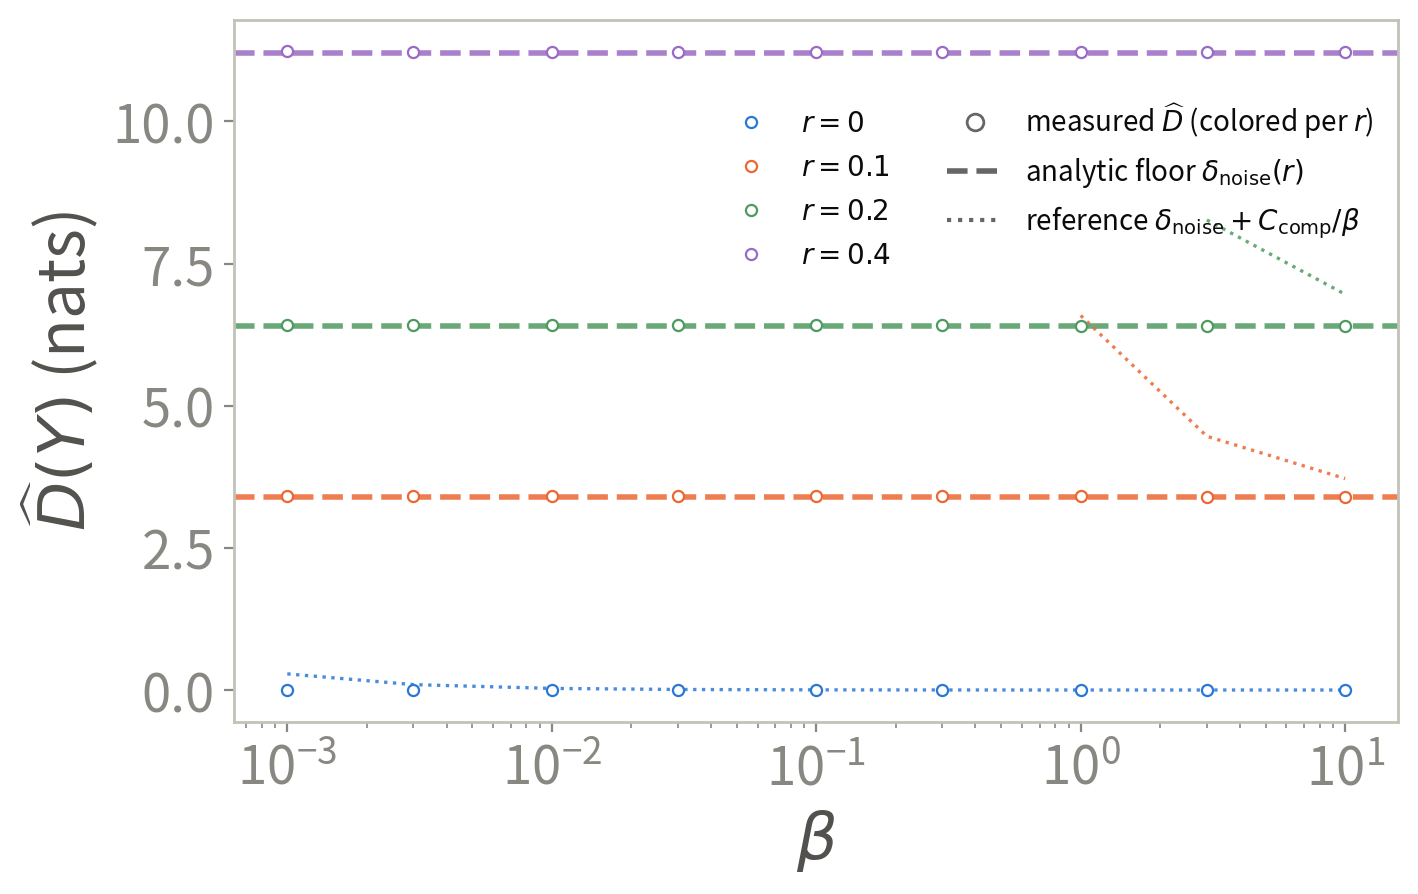
\includegraphics[width=0.32\linewidth]{figures/fig_noisy_appendix_i_varfixed.png}\hfill
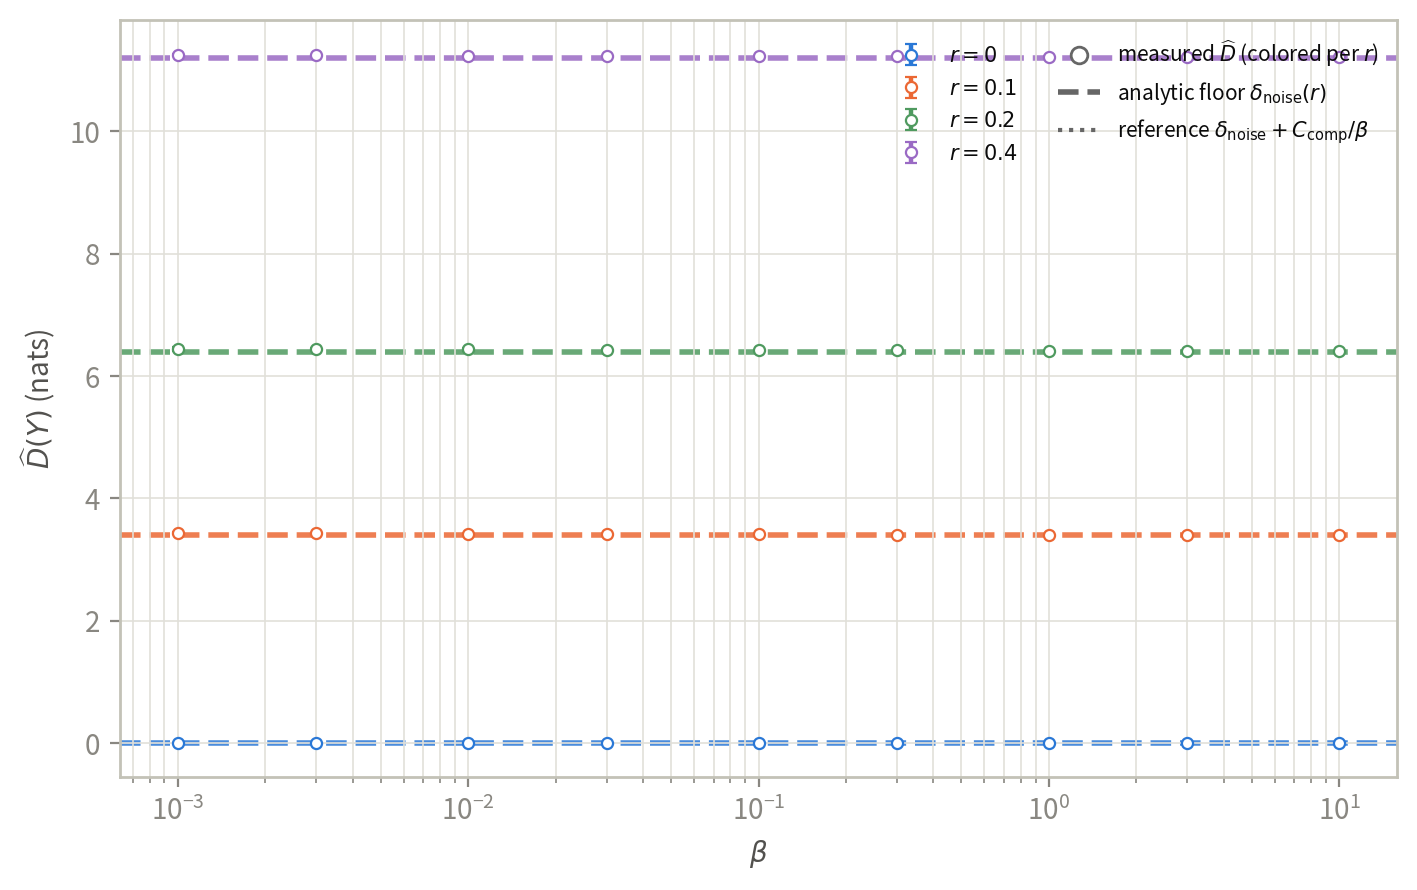
\includegraphics[width=0.32\linewidth]{figures/fig_noisy_appendix_ii_trainable.png}\hfill
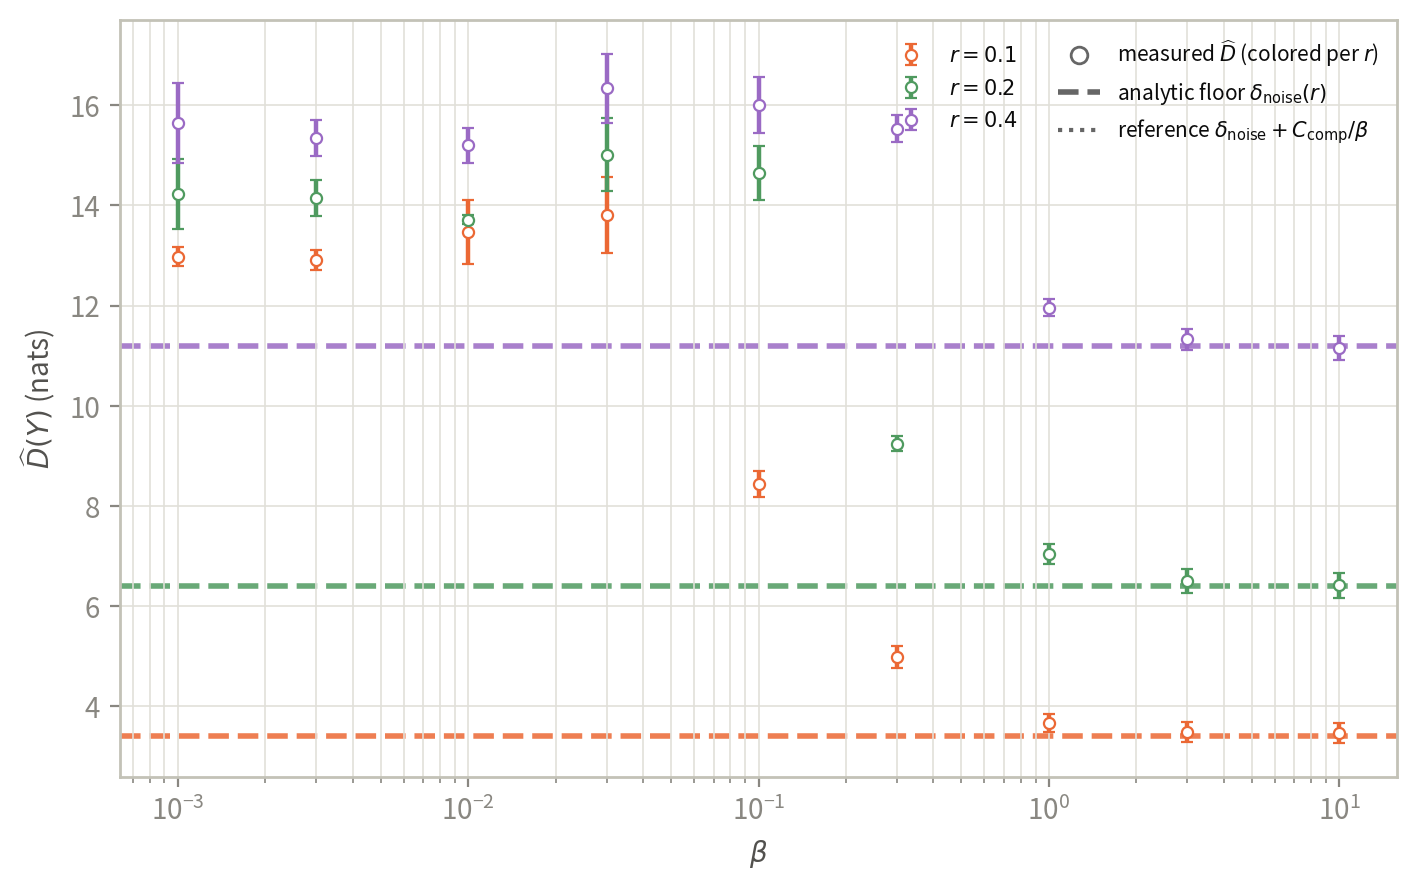
\includegraphics[width=0.32\linewidth]{figures/fig_noisy_appendix_iii_sampled.png}
\caption{Sensitivity analyses for the controlled label-ambiguity experiment.
(a) Posterior variance fixed to the prior variance. (b) Trainable polar
frame. (c) Labels sampled rather than integrated with their exact population weights;
failed comparator-gate configurations are marked. Dashed lines denote the analytic
population ambiguity floors. Points are means and error bars are standard deviations
over five seeds.}
\label{fig:noisy-alignment-sensitivity}
\end{figure*}

\subsection{Direct mismatch definitions and separation diagnostics}
\label{app:direct-mismatch}

This section collects the diagnostic panels deferred from
Section~\ref{sec:direct-mismatch}: the decoupling scatter, the separation-bound and
slack readings, and the regression diagnostics, together with the finite-bin
definitions. All statistics are first computed within each seed and then aggregated
across the five seeds; class or bin pairs are not treated as independent
replicates. The per-class Jensen check and the per-pair separation bound are
verified numerically on every scale, $\beta$, seed, and class (no violation exceeds
$10^{-6}$). Every checkpoint in both requested grids is present, and no collapse or
variance-explosion point is removed.

The deferred classification panels complete the picture
(Fig.~\ref{fig:direct-mismatch-deferred}). The decoupling scatter (a) shows MC-10
accuracy staying within $82$--$86\%$ while $\widehat D$ spans three orders of
magnitude: mechanism and task metric are decoupled. Panel (b) shows the raw bound
rising toward the declared $\sqrt2a$ exactly where the mismatch corrections shrink,
so the slack narrows where the bound is informative; CEB's mismatch is plotted
descriptively, without a bound or slack entries, since its reference has no declared
$\Delta$. The
slack percentiles (c) stay non-negative at every reported point: the bound is
consistent but conservative.

\begin{figure*}[t]
\centering
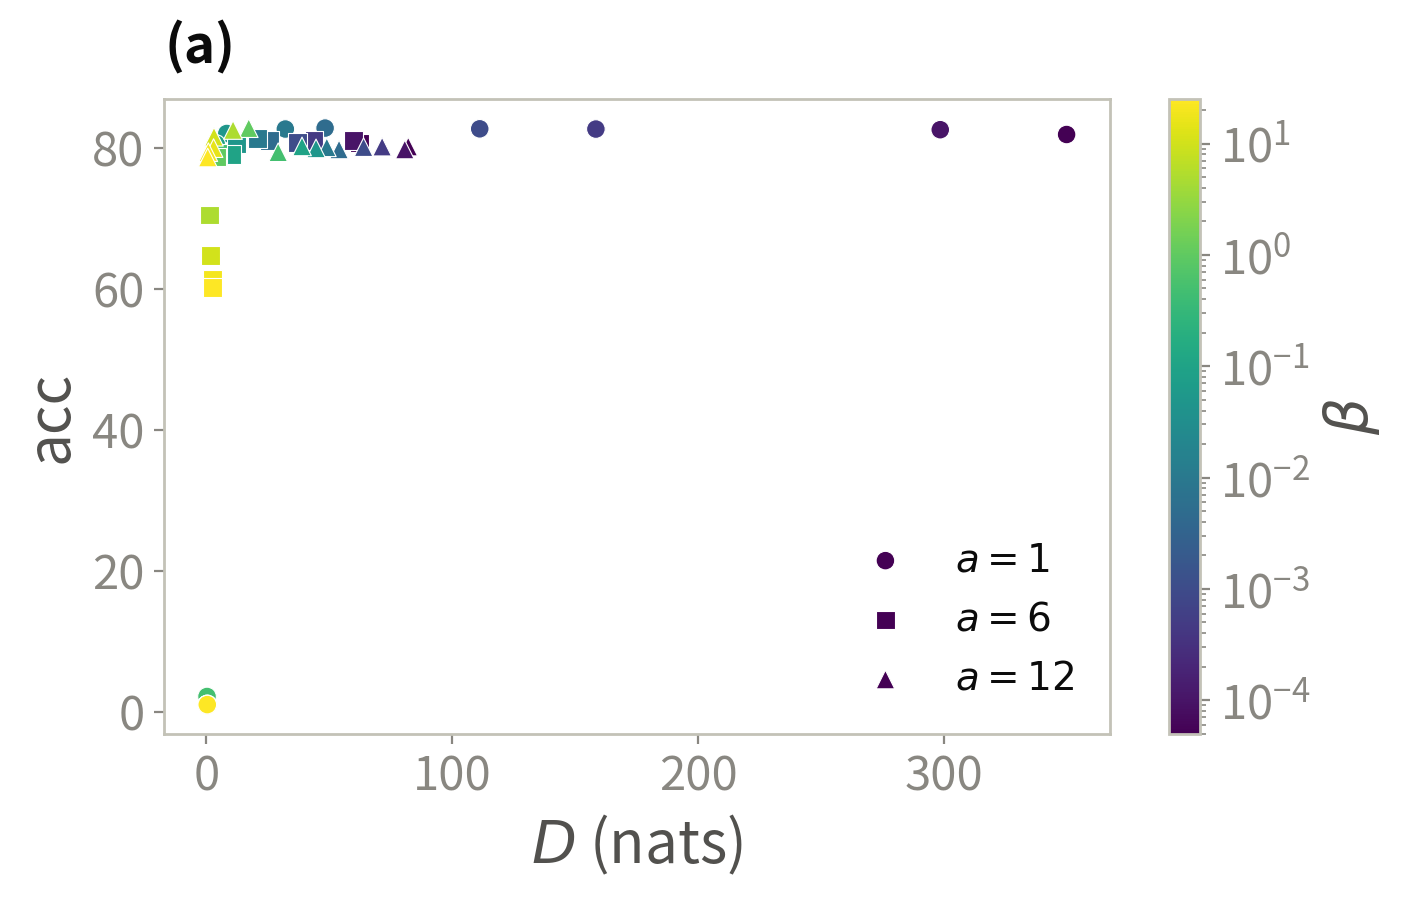
\includegraphics[width=0.24\linewidth]{figures/fig_mismatch_b_imagenet100_acc_vs_d.png}\hfill
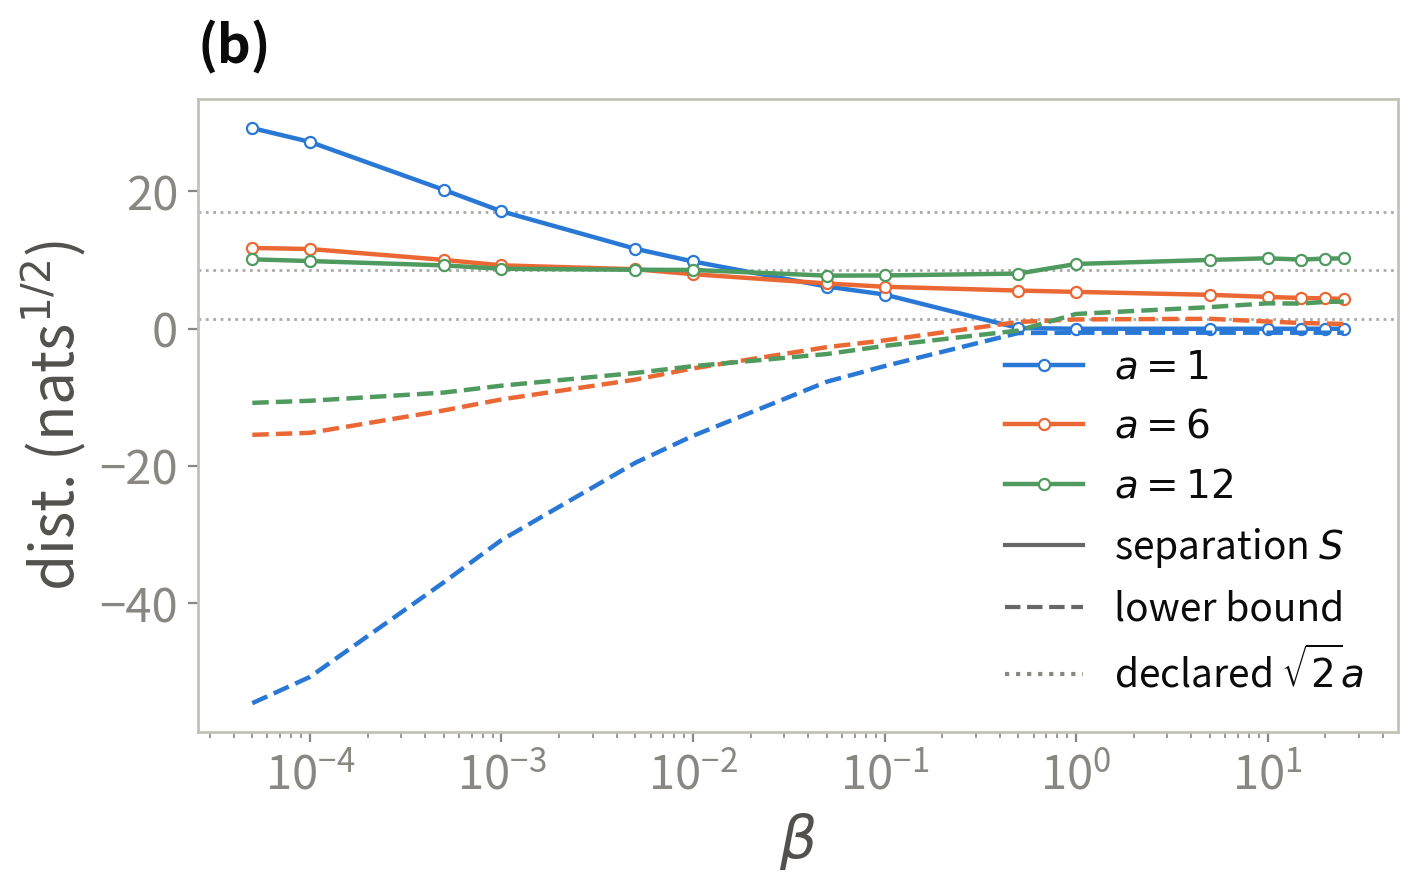
\includegraphics[width=0.24\linewidth]{figures/fig_mismatch_appendix_cls_i_separation_beta.png}\hfill
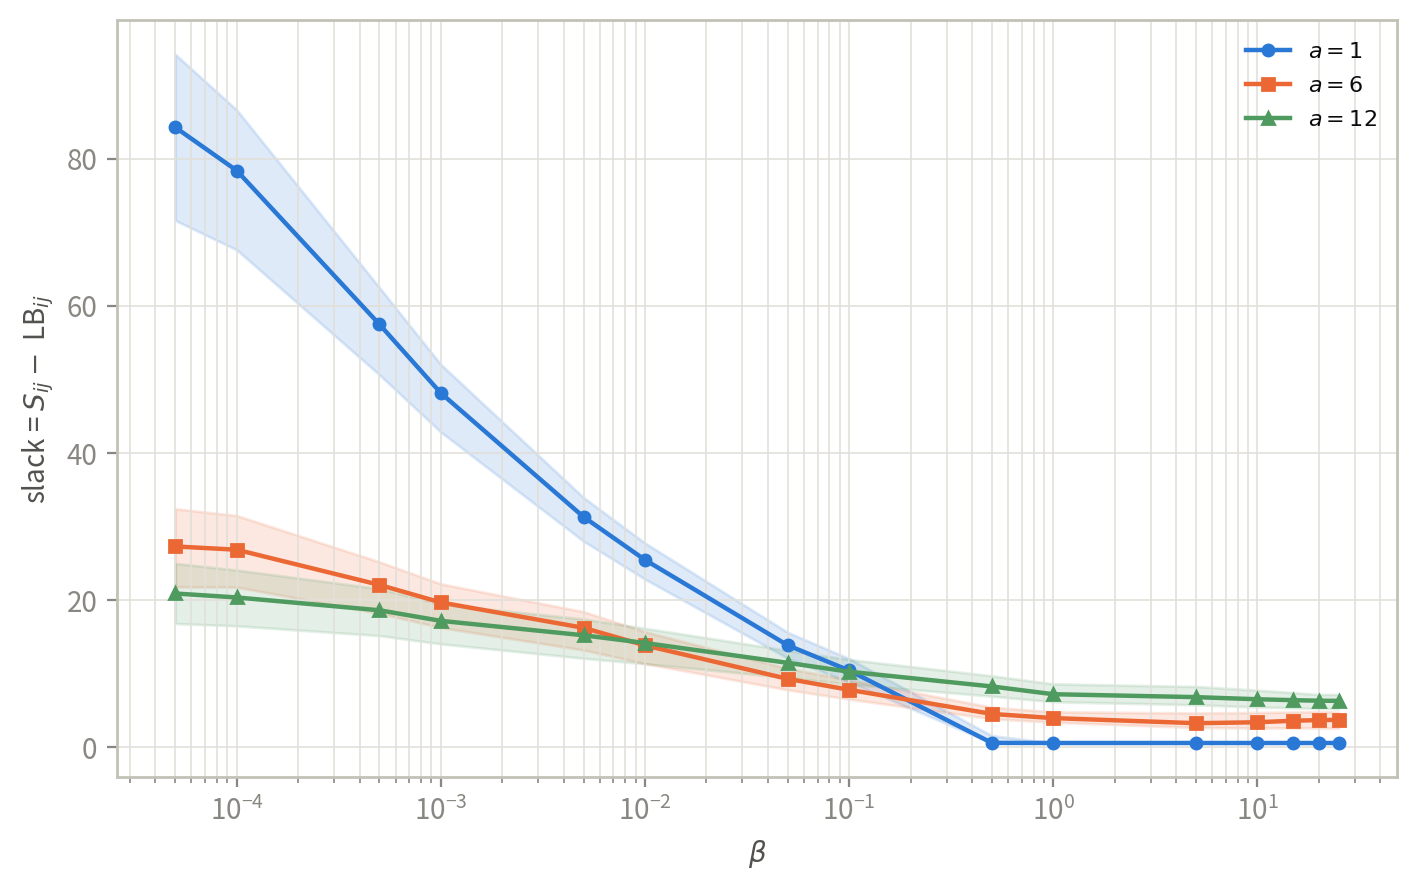
\includegraphics[width=0.24\linewidth]{figures/fig_mismatch_appendix_cls_iii_slack.png}\hfill
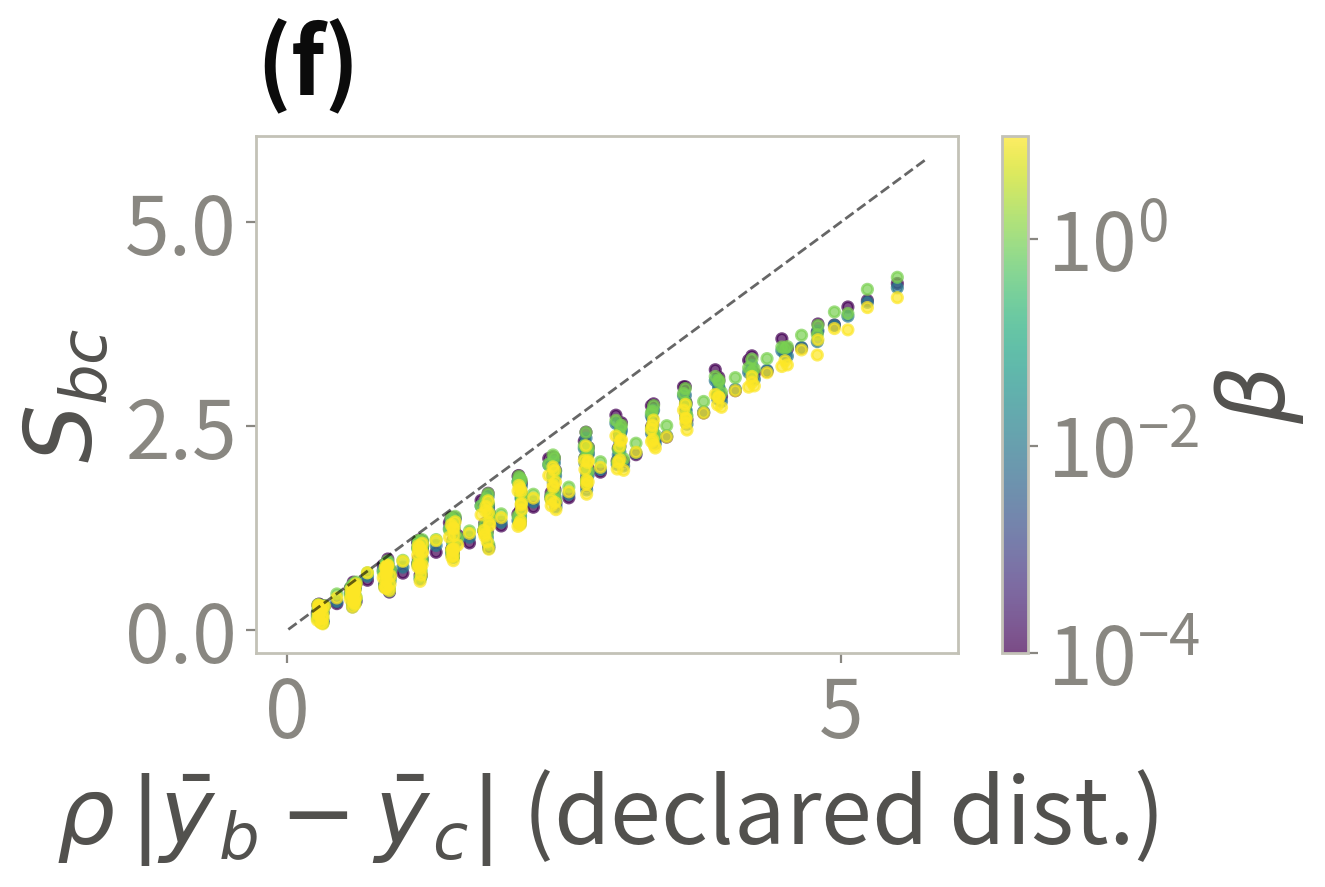
\includegraphics[width=0.24\linewidth]{figures/fig_mismatch_appendix_reg_binscatter.png}
\caption{Direct mismatch diagnostics deferred from the main text. (a) MC-10
accuracy against $\widehat D$ (color $=\beta$, marker $=a$). (b) Mean separation
(solid) and raw lower bound (dashed) against $\beta$; gray dotted: CEB,
descriptive. (c) Slack percentiles. (d) Cal.\ Housing bin-pair separation against
the declared prior distance at $\rho=6$ (color $=\beta$; identity line: exact
transfer). Means and standard deviations are over five seeds; no checkpoint is
omitted.}
\label{fig:direct-mismatch-deferred}
\end{figure*}

\paragraph{Regression.} We partition the standardized test labels into $20$
equal-width bins and merge any bin containing fewer than $30$ examples. Let
$\bar y_b$ be the mean label of bin $B_b$, $\widehat m_b$ its posterior center,
$\widehat D_b$ its average sample-to-own-anchor mismatch, and
$h_b:=\operatorname{diam}(B_b)$. The finite-bin lower bound is
\begin{equation}
\widehat{\mathrm{LB}}_{bc}
=\rho|\bar y_b-\bar y_c|
-\sqrt{2\tau^2\widehat D_b}
-\sqrt{2\tau^2\widehat D_c}
-\rho(h_b+h_c),
\label{eq:empirical-regression-separation-bound}
\end{equation}
where the last term is the quantization correction of
Remark~\ref{rem:pgib-binning}. On Housing with $\rho=6$, mismatch falls from
$0.264$ to $0.026$, the axial slope remains $0.73$--$0.77$, and the mismatch is
almost entirely axial (about $0.2$ against $0.004$ off-axis), while $R^2$ changes
only from $0.786$ to $0.767$ over the sweep: a tenfold mismatch reduction need not
imply a comparable task-metric gain. Figure~\ref{fig:direct-mismatch-deferred}d
plots the actual bin-center distances against the declared isometric distances at
$\rho=6$: the cloud hugs a line of slope $0.73$--$0.77$ below the identity line at
all four $\beta$ values, so the posterior follows the declared metric structure at
about three quarters of its scale, and the scale-transfer ratio is essentially
$\beta$-invariant. After the quantization correction, $43\%$ of bin pairs retain a
positive bound. Figure~\ref{fig:direct-mismatch-housing} shows the two regression
sweep panels: the mismatch--$\beta$ curves with their axial/off-axis decomposition
(the dotted off-axis contribution stays below $0.01$ nats, so the posterior lies
essentially on the declared axis), and the $R^2$-against-$\widehat D$ scatter whose
band stays within $0.75$--$0.79$ while $\widehat D$ spans orders of magnitude.

\begin{figure*}[t]
\centering
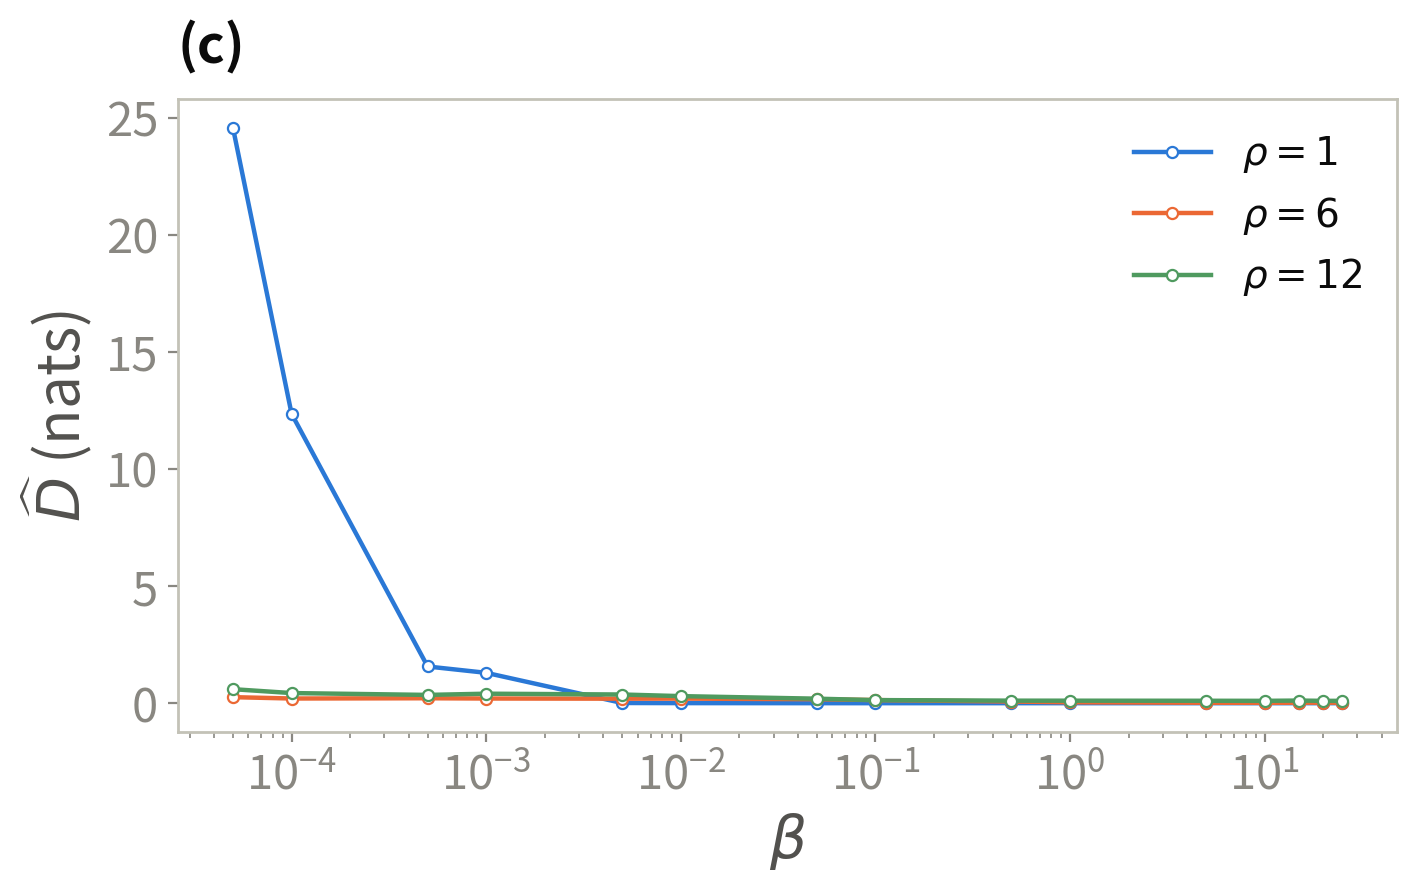
\includegraphics[width=0.48\linewidth]{figures/fig_mismatch_c_housing_d_beta.png}\hfill
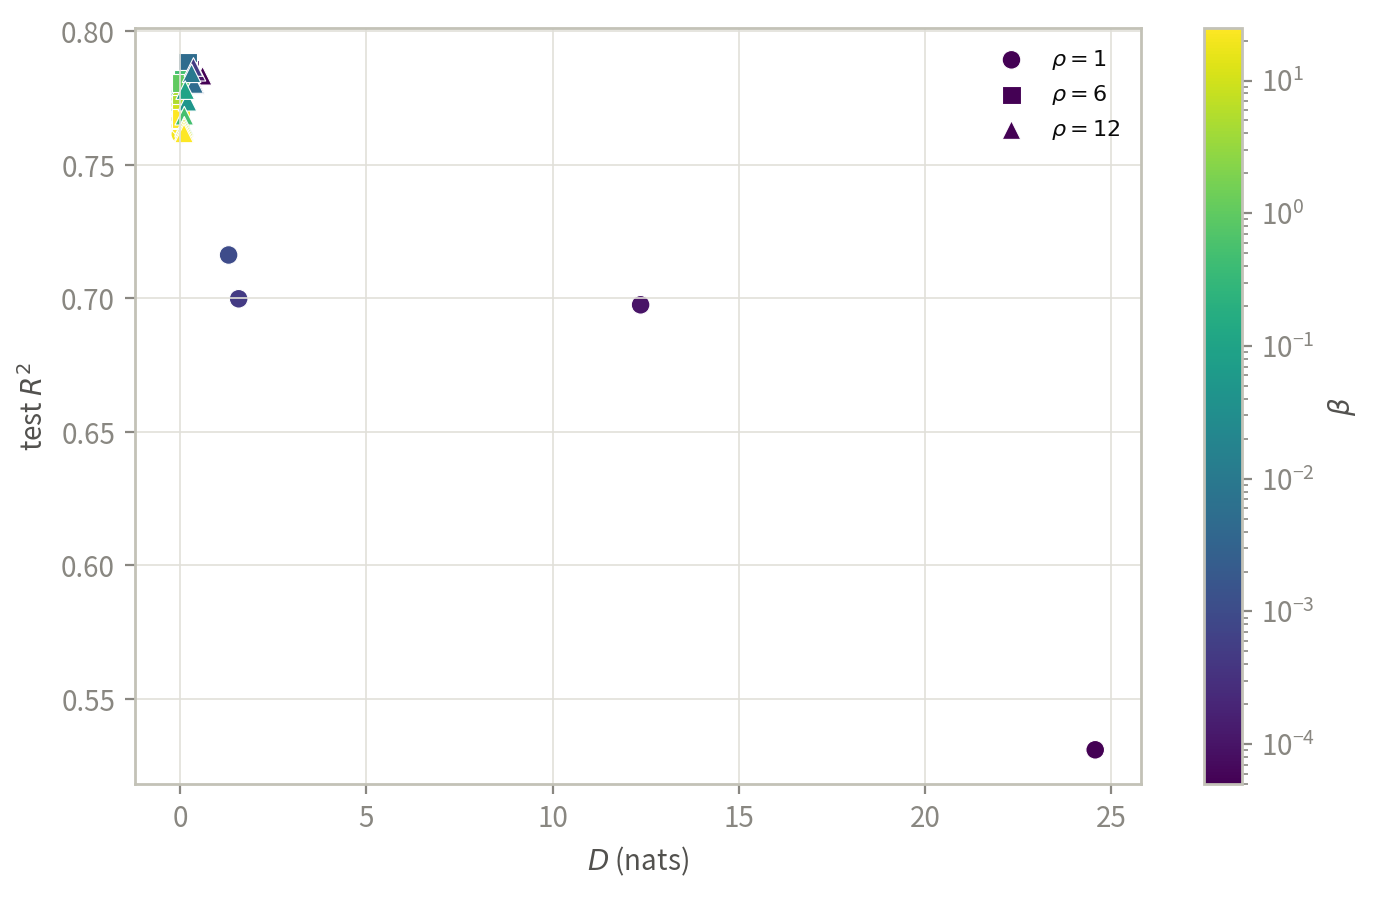
\includegraphics[width=0.48\linewidth]{figures/fig_mismatch_d_housing_r2_vs_d.png}
\caption{Cal.\ Housing mismatch sweep panels (deferred from the main text). (a)
Anchor mismatch $\widehat D$ against $\beta$, by isometric scale $\rho$, decomposed
into axial and off-axis contributions. (b) Test $R^2$ against $\widehat D$; color
denotes $\beta$ and marker shape $\rho$. Means and standard deviations are over five
seeds; no checkpoint is omitted.}
\label{fig:direct-mismatch-housing}
\end{figure*}

\paragraph{Normalization and variance extremes.} The empirical mismatch normalizes
by the declared prior variance $\tau^2=1$, whereas the
exact Gaussian KL uses every sample's and coordinate's own posterior variance
$\sigma^2_\phi(x)$. They therefore need not coincide: averaged over the ImageNet-100
grid, $\widehat D=41.2$, the KL mean term is $46.5$, and the KL variance term is
$51.4$. On Housing, a small number of weak-compression, large-$\rho$ posterior
variance explosions raise the across-grid mean KL variance term to $2.8\times10^6$;
these checkpoints remain in all plots. The unnormalized axial/off-axis components and
total KL are therefore reported alongside $\widehat D$.

\subsection{Main results with standard deviations}
\label{app:main-std}

Tables~\ref{tab:main_result_std_baselines} and~\ref{tab:main_result_std_variants}
report the same configurations as the main table with standard deviations over
runs, split by column groups for width (the baselines table includes NCBD and the
variants table includes AdaCap); bold and underline follow the same
mean-based rule as Table~\ref{tab:main_result}.

% 主结果表（带标准差）：由 paper/make_table.py 从 tune_results/*.html 自动生成，请勿手改。
% 因 8 方法列 × (均值±std) 超出页宽，按列拆为两张表：
% (a) baselines（Base/VIB/SVIB/NIB，tab:main_result_std_baselines）；
% (b) CEB/DVCCA 与 GPB/GPB-L（tab:main_result_std_variants，竖线分隔同主表）。
% 每表含全部 12 行；分类 Acc（%）、回归 R²，单元格为均值±std；
% 加粗/下划线按该行全部 8 列的均值判定（与 main_result.tex 一致）；
% 表尾排名行省略（与主表重复）。
\begin{table*}[t]
\centering
\caption{Test accuracy (\%) and test $R^2$ with standard deviations over runs: the plain backbone and the variational baselines; same configurations as Table~\ref{tab:main_result}.}
\label{tab:main_result_std_baselines}
\small
{
\setlength{\tabcolsep}{2pt}
\begin{tabular}{llcccc}
\hline
Dataset & Backbone & Base & VIB & SVIB & NIB \\
\hline
MNIST & MLP & 98.33$\pm$0.12 & 98.28$\pm$0.11 & 98.15$\pm$0.13 & 98.27$\pm$0.07 \\
MNIST & CNN & 99.13$\pm$0.05 & 99.28$\pm$0.09 & 99.23$\pm$0.03 & 99.22$\pm$0.06 \\
ImageNet-100 & MLP & 83.12$\pm$0.14 & 82.84$\pm$0.44 & 83.02$\pm$0.37 & 82.35$\pm$0.27 \\
ImageNet-100 & CNN & 83.40$\pm$0.13 & 82.94$\pm$0.37 & 83.11$\pm$0.86 & 82.91$\pm$0.35 \\
Cora & GCN & 87.68$\pm$0.46 & 86.83$\pm$0.28 & 86.46$\pm$1.87 & 86.35$\pm$0.68 \\
IMDb & RNN & 84.85$\pm$0.68 & 85.50$\pm$0.91 & 85.99$\pm$0.30 & 86.14$\pm$0.92 \\
AG News & RNN & \textbf{92.94$\pm$0.15} & 92.72$\pm$0.17 & 92.86$\pm$0.21 & 92.91$\pm$0.22 \\
\hline\hline
Cal. Housing & MLP & 0.7618$\pm$0.0238 & \underline{0.7901$\pm$0.0049} & 0.7897$\pm$0.0058 & 0.7862$\pm$0.0035 \\
STS-B & RNN & \textbf{0.2899$\pm$0.0113} & 0.2719$\pm$0.0164 & 0.2697$\pm$0.0202 & 0.2417$\pm$0.0221 \\
ZINC & GCN & \textbf{0.6348$\pm$0.0044} & 0.6339$\pm$0.0033 & 0.6325$\pm$0.0026 & 0.6178$\pm$0.0099 \\
AgeDB & MLP & 0.2180$\pm$0.0409 & 0.3173$\pm$0.0101 & \underline{0.3385$\pm$0.0286} & 0.2710$\pm$0.0235 \\
AgeDB & CNN & 0.3914$\pm$0.0194 & 0.3342$\pm$0.1894 & 0.3323$\pm$0.1870 & 0.3337$\pm$0.1889 \\
\hline
\end{tabular}
}
\end{table*}
\par\smallskip
\begin{table*}[t]
\centering
\caption{Test accuracy (\%) and test $R^2$ with standard deviations over runs: CEB, DVCCA, and our method; same configurations as Table~\ref{tab:main_result}. GPB and GPB-L are separated from the references by the vertical rule.}
\label{tab:main_result_std_variants}
\small
{
\setlength{\tabcolsep}{2pt}
\begin{tabular}{llcc|cc}
\hline
Dataset & Backbone & CEB & DVCCA & GPB & GPB-L \\
\hline
MNIST & MLP & \underline{98.43$\pm$0.08} & 98.24$\pm$0.17 & \textbf{98.54$\pm$0.09} & \underline{98.43$\pm$0.07} \\
MNIST & CNN & 99.30$\pm$0.05 & 99.29$\pm$0.10 & \textbf{99.32$\pm$0.05} & \underline{99.31$\pm$0.05} \\
ImageNet-100 & MLP & 82.77$\pm$0.22 & 82.99$\pm$0.43 & \textbf{84.40$\pm$0.21} & \underline{84.01$\pm$0.23} \\
ImageNet-100 & CNN & 82.97$\pm$0.67 & 83.21$\pm$0.70 & \textbf{86.08$\pm$0.21} & \underline{84.88$\pm$0.80} \\
Cora & GCN & 86.27$\pm$0.38 & 86.90$\pm$0.94 & \textbf{88.12$\pm$0.55} & \underline{87.86$\pm$0.87} \\
IMDb & RNN & 85.55$\pm$0.73 & 85.69$\pm$0.23 & \underline{86.84$\pm$0.57} & \textbf{86.99$\pm$0.35} \\
AG News & RNN & 92.83$\pm$0.11 & 92.78$\pm$0.15 & 92.87$\pm$0.12 & \underline{92.92$\pm$0.14} \\
\hline\hline
Cal. Housing & MLP & 0.7894$\pm$0.0018 & 0.7878$\pm$0.0048 & 0.7895$\pm$0.0051 & \textbf{0.7914$\pm$0.0034} \\
STS-B & RNN & 0.2668$\pm$0.0127 & 0.2713$\pm$0.0218 & \underline{0.2762$\pm$0.0152} & 0.2755$\pm$0.0134 \\
ZINC & GCN & 0.6257$\pm$0.0044 & 0.6294$\pm$0.0026 & \underline{0.6344$\pm$0.0031} & 0.6323$\pm$0.0016 \\
AgeDB & MLP & 0.3317$\pm$0.0251 & 0.3180$\pm$0.0228 & \textbf{0.3536$\pm$0.0076} & 0.3320$\pm$0.0080 \\
AgeDB & CNN & 0.3882$\pm$0.0275 & 0.3205$\pm$0.1811 & \textbf{0.4700$\pm$0.0072} & \underline{0.4388$\pm$0.0220} \\
\hline
\end{tabular}
}
\end{table*}
\par\smallskip


\subsection{Paired-difference confidence intervals}
\label{app:main-ci}

Tables~\ref{tab:main_result_ci_baselines}--\ref{tab:main_result_ci_external}
report, for each setting, the paired difference of GPB over every baseline
(GPB minus baseline) with a bootstrap $95\%$ confidence interval: the differences
are paired across the shared seeds, the interval is the percentile interval of
$B = 10{,}000$ resamples of the per-run differences (fixed seed, reproducible), and
the non-inferiority margin is $\delta = 0.2$ percentage points of accuracy or
$\delta = 0.005$ in $R^2$. Bold marks a lower bound above zero (significant
advantage) and $^{\dagger}$ a lower bound within the margin (tied); the best
configuration per method is the same as in the main table. The last table covers
the external non-IB baselines, NCBD on the classification settings and AdaCap on
the regression settings; the only interval lying entirely below zero is AdaCap on
ZINC ($-0.043$ $R^2$).

% 主结果差值 CI 表：由 paper/make_table.py 从 tune_results 自动生成，请勿手改。
% 行 = 12 个 setting；单元格 = GPB − baseline 的配对差值 [bootstrap 95% CI]
%（分类百分点、回归 R²）；加粗 = CI 下限 > 0（显著更优）、† = CI 下限 > −δ
%（非劣界 δ=0.2 百分点 / 0.005）记 tied；
% 同 seed 配对（run 顺序即 seed 0..N−1），bootstrap B=10000（固定 seed 0，百分位法）。
% 因 7 个差值列超页宽，按列拆两张表（baselines / ceb+dvcca+OPB-L）；表尾一行统计各列 */† 次数。
\begin{table*}[t]
\centering
\caption{Paired-difference 95\% confidence intervals of GPB over the plain backbone and VIB (GPB minus baseline, per setting; classification in percentage points, regression in $R^2$). Bold: lower CI bound above zero; $^{\dagger}$: lower bound within the non-inferiority margin $\delta$ (tied).}
\label{tab:main_result_ci_baselines}
\small
{
\setlength{\tabcolsep}{1pt}
\begin{tabular}{llcc}
\hline
Dataset & Backbone & Base & VIB \\
\hline
MNIST & MLP & \textbf{+0.2 [+0.2, +0.3]} & \textbf{+0.3 [+0.2, +0.3]} \\
MNIST & CNN & \textbf{+0.2 [+0.2, +0.2]} & +0.0 [-0.0, +0.1]$^{\dagger}$ \\
ImageNet-100 & MLP & \textbf{+1.3 [+1.2, +1.4]} & \textbf{+1.6 [+1.4, +1.9]} \\
ImageNet-100 & CNN & \textbf{+2.7 [+2.5, +2.9]} & \textbf{+3.1 [+3.0, +3.4]} \\
Cora & GCN & +0.4 [-0.1, +1.1]$^{\dagger}$ & \textbf{+1.3 [+0.7, +1.7]} \\
IMDb & RNN & \textbf{+2.0 [+1.2, +2.7]} & \textbf{+1.3 [+0.6, +2.3]} \\
AG News & RNN & -0.1 [-0.2, +0.0]$^{\dagger}$ & \textbf{+0.2 [+0.1, +0.2]} \\
\hline\hline
Cal. Housing & MLP & \textbf{+0.028 [+0.008, +0.048]} & -0.001 [-0.005, +0.003]$^{\dagger}$ \\
STS-B & RNN & -0.014 [-0.022, -0.006] & +0.004 [-0.017, +0.022] \\
ZINC & GCN & -0.000 [-0.003, +0.002]$^{\dagger}$ & +0.001 [-0.004, +0.004]$^{\dagger}$ \\
AgeDB & MLP & \textbf{+0.136 [+0.104, +0.167]} & \textbf{+0.036 [+0.026, +0.046]} \\
AgeDB & CNN & \textbf{+0.079 [+0.066, +0.091]} & \textbf{+0.136 [+0.043, +0.302]} \\
\hline
 &  & 8*/3† & 8*/3† \\
\hline
\end{tabular}
}
\end{table*}
\par\smallskip
\begin{table*}[t]
\centering
\caption{Paired-difference 95\% confidence intervals of GPB over SVIB and NIB (GPB minus baseline, per setting; classification in percentage points, regression in $R^2$). Bold/† as in the baselines table.}
\label{tab:main_result_ci_svib_nib}
\small
{
\setlength{\tabcolsep}{1pt}
\begin{tabular}{llcc}
\hline
Dataset & Backbone & SVIB & NIB \\
\hline
MNIST & MLP & \textbf{+0.4 [+0.3, +0.5]} & \textbf{+0.3 [+0.2, +0.3]} \\
MNIST & CNN & \textbf{+0.1 [+0.1, +0.1]} & \textbf{+0.1 [+0.1, +0.2]} \\
ImageNet-100 & MLP & \textbf{+1.4 [+1.1, +1.7]} & \textbf{+2.1 [+1.8, +2.2]} \\
ImageNet-100 & CNN & \textbf{+3.0 [+2.4, +3.9]} & \textbf{+3.2 [+2.9, +3.5]} \\
Cora & GCN & \textbf{+1.7 [+0.2, +3.4]} & \textbf{+1.8 [+1.1, +2.4]} \\
IMDb & RNN & \textbf{+0.8 [+0.2, +1.4]} & \textbf{+0.7 [+0.2, +1.2]} \\
AG News & RNN & +0.0 [-0.1, +0.1]$^{\dagger}$ & -0.0 [-0.2, +0.1]$^{\dagger}$ \\
\hline\hline
Cal. Housing & MLP & -0.000 [-0.006, +0.004] & +0.003 [-0.001, +0.009]$^{\dagger}$ \\
STS-B & RNN & +0.006 [-0.021, +0.028] & \textbf{+0.035 [+0.011, +0.058]} \\
ZINC & GCN & +0.002 [-0.001, +0.004]$^{\dagger}$ & \textbf{+0.017 [+0.010, +0.026]} \\
AgeDB & MLP & +0.015 [-0.010, +0.041] & \textbf{+0.083 [+0.062, +0.100]} \\
AgeDB & CNN & \textbf{+0.138 [+0.045, +0.303]} & \textbf{+0.136 [+0.040, +0.302]} \\
\hline
 &  & 7*/2† & 10*/2† \\
\hline
\end{tabular}
}
\end{table*}
\par\smallskip
\begin{table*}[t]
\centering
\caption{Paired-difference 95\% confidence intervals of GPB over CEB, DVCCA, and the free-head ablation OPB-L (GPB minus baseline, per setting; classification in percentage points, regression in $R^2$). Bold/† as in the baselines table.}
\label{tab:main_result_ci_variants}
\small
{
\setlength{\tabcolsep}{1pt}
\begin{tabular}{llccc}
\hline
Dataset & Backbone & CEB & DVCCA & OPB-L \\
\hline
MNIST & MLP & \textbf{+0.1 [+0.0, +0.2]} & \textbf{+0.3 [+0.2, +0.4]} & \textbf{+0.1 [+0.0, +0.2]} \\
MNIST & CNN & +0.0 [-0.0, +0.1]$^{\dagger}$ & +0.0 [-0.1, +0.1]$^{\dagger}$ & +0.0 [-0.0, +0.1]$^{\dagger}$ \\
ImageNet-100 & MLP & \textbf{+1.6 [+1.5, +1.7]} & \textbf{+1.4 [+1.1, +1.7]} & \textbf{+0.4 [+0.2, +0.5]} \\
ImageNet-100 & CNN & \textbf{+3.1 [+2.4, +3.7]} & \textbf{+2.9 [+2.4, +3.5]} & \textbf{+1.2 [+0.5, +1.9]} \\
Cora & GCN & \textbf{+1.8 [+1.5, +2.3]} & \textbf{+1.2 [+0.4, +1.9]} & +0.3 [-0.5, +1.3] \\
IMDb & RNN & \textbf{+1.3 [+0.3, +2.1]} & \textbf{+1.1 [+0.8, +1.5]} & -0.2 [-0.6, +0.5] \\
AG News & RNN & +0.0 [-0.1, +0.2]$^{\dagger}$ & +0.1 [-0.0, +0.2]$^{\dagger}$ & -0.0 [-0.2, +0.1]$^{\dagger}$ \\
\hline\hline
Cal. Housing & MLP & +0.000 [-0.003, +0.004]$^{\dagger}$ & +0.002 [-0.005, +0.009] & -0.002 [-0.005, +0.002] \\
STS-B & RNN & +0.009 [-0.009, +0.025] & +0.005 [-0.020, +0.026] & +0.001 [-0.019, +0.017] \\
ZINC & GCN & \textbf{+0.009 [+0.005, +0.011]} & \textbf{+0.005 [+0.002, +0.007]} & +0.002 [-0.001, +0.005]$^{\dagger}$ \\
AgeDB & MLP & \textbf{+0.022 [+0.006, +0.038]} & \textbf{+0.036 [+0.012, +0.057]} & \textbf{+0.022 [+0.019, +0.025]} \\
AgeDB & CNN & \textbf{+0.082 [+0.064, +0.099]} & \textbf{+0.149 [+0.065, +0.310]} & \textbf{+0.031 [+0.018, +0.046]} \\
\hline
 &  & 8*/3† & 8*/2† & 5*/3† \\
\hline
\end{tabular}
}
\end{table*}
\par\smallskip


\subsection{Information-plane panels for Cal.~Housing}
\label{app:info-plane-extra}

Figure~\ref{fig:info-plane-extra} completes panels (c)--(d) of
Fig.~\ref{fig:compression-main} in the main text with the regression setting, under
the same $\beta$ grid, axis
conventions, and five runs per point; here
$I(Y;Z)$ is the Gaussian approximation
$\tfrac12 \ln\bigl(\mathrm{Var}(y)/\mathrm{Var}(y-\hat y)\bigr)$, a heuristic
rather than a bound. On Cal.~Housing this approximation consistently reads
above the InfoNCE bound, so the certificate panel reflects the estimator gap
rather than the geometry; the information plane remains informative: CEB
compresses itself off the task ($R^2 = 0.49$ at $\beta = 0.1$, $0.18$ at
$\beta = 0.5$) while every EPB curve keeps $R^2 \ge 0.76$ flat out to
$\beta = 25$.

\begin{figure*}[t]
\centering
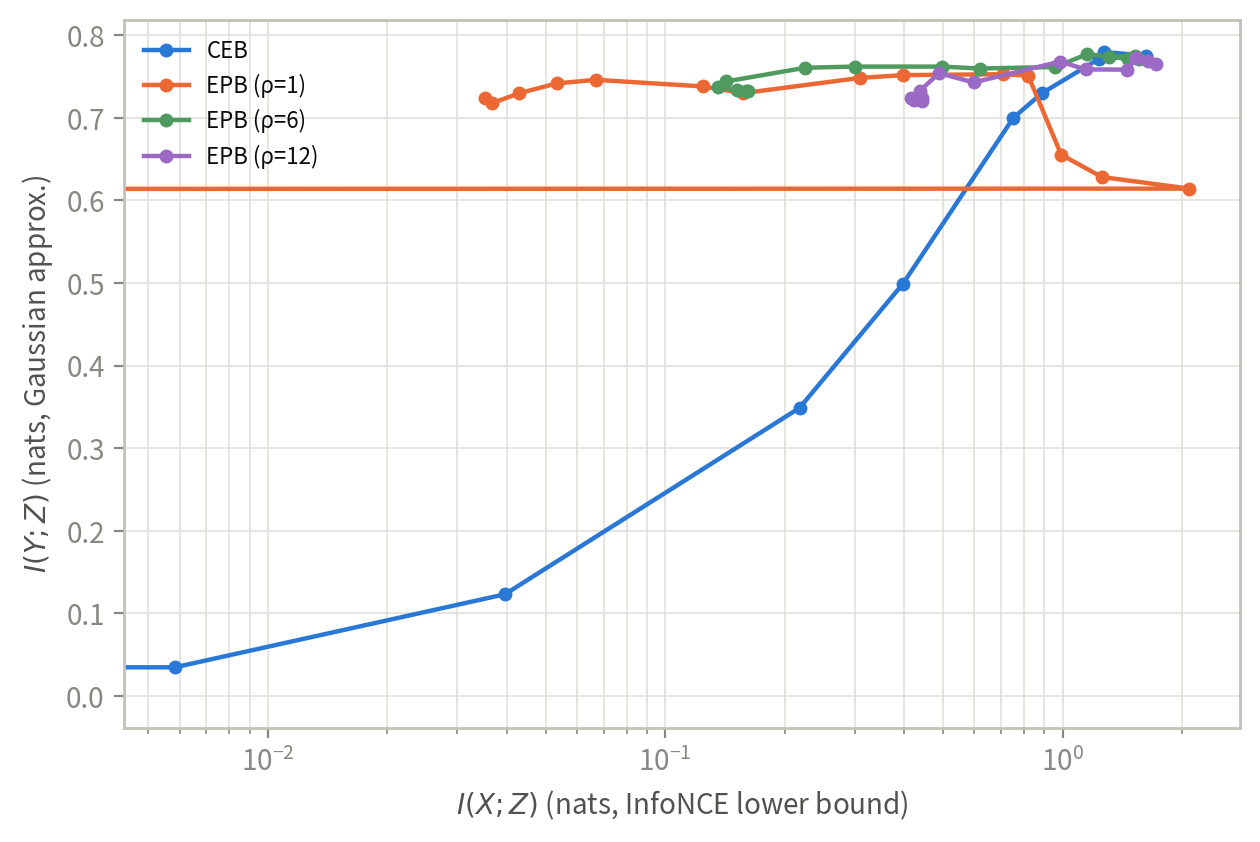
\includegraphics[width=0.48\linewidth]{figures/fig_info_plane_housing.png}\hfill
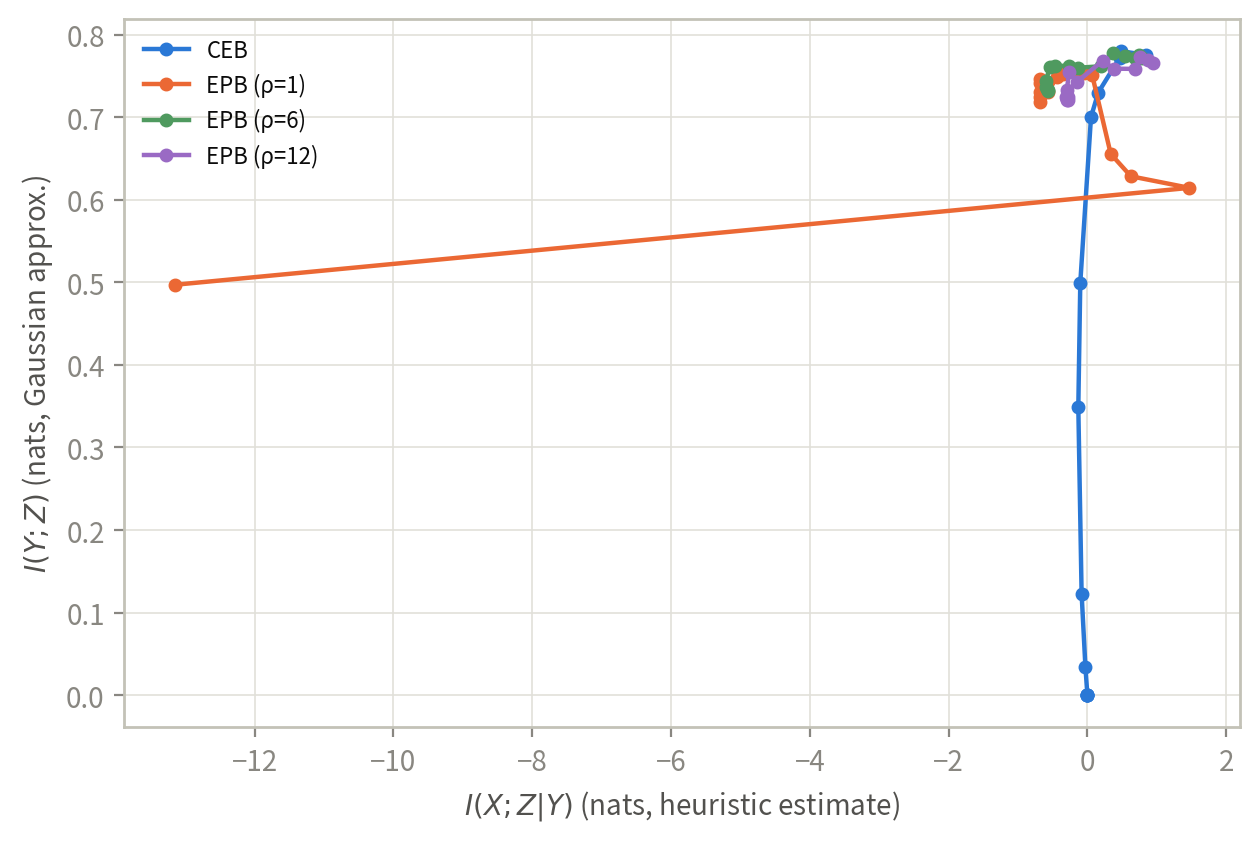
\includegraphics[width=0.48\linewidth]{figures/fig_certificate_plane_housing.png}
\caption{Information plane (a) and certificate plane (b) for Cal.~Housing,
companion panels to Fig.~\ref{fig:compression-main}(c,d): identical estimators,
$\beta$ grid (log $x$-scale in (a); linear where the estimated residual turns negative
in (b)), five runs per point, lines connect $\beta$ in ascending order. CEB
one curve per panel; EPB three ($\rho \in \{1, 6, 12\}$).}
\label{fig:info-plane-extra}
\end{figure*}

% =====================================================================
：诊断/证明/构造细节/补充结果）。
% 相关工作由 related_work.tex 单独维护，并在正文中通过 \input 引入。

\documentclass{article} % For LaTeX2e
\usepackage{iclr2027_conference,times}

% Optional math commands from https://github.com/goodfeli/dlbook_notation.
\input{math_commands.tex}

\usepackage{hyperref}
\usepackage{url}

% 本文所需扩展（不影响模板版式参数）：amsmath 用于 multline/gathered，
% 定理环境、emergencystretch 兜底行溢出、\KL 覆写为本文的 KL(·‖·) 记法
% （math_commands.tex 默认定义为 D_KL 形式）。
\usepackage{amsmath,amssymb,amsthm}
\usepackage{graphicx} % 机制验证图（fig:mechanism，两张 PNG 从机制报告 HTML 导出）
\emergencystretch=1.5em
\theoremstyle{plain}
\newtheorem{theorem}{Theorem}[section]
\newtheorem{proposition}{Proposition}[section]
\newtheorem{lemma}{Lemma}[section]
\newtheorem{corollary}{Corollary}[section]
\newtheorem{assumption}{Assumption}[section]
\theoremstyle{remark}
\newtheorem{remark}{Remark}[section]
\renewcommand{\KL}{\operatorname{KL}}
\DeclareMathOperator{\CE}{CE}

\title{Geometry by Construction: A Geometric Prior Bottleneck}

% Authors must not appear in the submitted version. They should be hidden
% as long as the \iclrfinalcopy macro remains commented out below.
% Non-anonymous submissions will be rejected without review.
\author{Anonymous authors}

\newcommand{\fix}{\marginpar{FIX}}
\newcommand{\new}{\marginpar{NEW}}

%\iclrfinalcopy % Uncomment for camera-ready version, but NOT for submission.

\begin{document}

\maketitle

\begin{abstract}
The conditional entropy bottleneck (CEB) compresses representations against a
label-conditional reference whose geometry is left entirely to the optimizer. We
show that this reference has two failure channels: in deterministic settings the
CEB knob is dead (a known Caveat), and, more fundamentally, the certificate is
blind to the relationships between labels: no cross-class term constrains the
geometry among the class priors. We close this channel by declaring the geometry:
the prior is confined to a qualified geometric family computed statelessly at
every training step: an orthogonal class frame (OPB) for classification and an
isometric regression axis (EPB) for regression, both with prediction rules tied
to the geometry by construction (the zero-parameter anchor-energy classifier and
the tied projection head). The framework preserves the CEB certificate for any
stateless conditional prior and yields a comparator-dependent alignment bound for
arbitrary label noise and model misspecification. Its residual floor separates
irreducible label ambiguity, encoder approximation, and covariance mismatch; the
exact $O(1/\beta)$ rate is recovered only as the noiseless, exactly realizable special
case. A controlled known-noise experiment recovers the predicted non-zero floors at
three noise levels and the zero floor when labels are deterministic. Independently of
this optimization bound, the observed anchor mismatch transfers the declared prior
separation to the posterior. At the strongest reported compression, direct benchmark
diagnostics show this bound is informative for $96.9\%$ of ImageNet-100 class pairs
with the largest anchors, while the regression bound is consistent but often vacuous.
The construction removes the unspecified
inter-class geometry of the reference. Across
nine datasets and four backbones, GPB is best or tied-best in $7$ of $12$ settings
and dominates CEB everywhere, and the anchor scale converts the $\beta$-knob from
a collapse dial into a plateau dial.
\end{abstract}


% =====================================================================
\section{Introduction}
% =====================================================================

The information bottleneck (IB) principle \citep{tishby2000information} seeks a
representation $Z$ of an input $X$ that retains the information needed to predict the
label $Y$ while discarding the rest. The variational IB (VIB) \citep{alemi2017deep}
bounds the compression term with a fixed marginal prior $\mathcal{N}(0,I)$; the
conditional entropy bottleneck (CEB) \citep{fischer2020conditional} sharpens the bound
to the residual information by replacing the marginal prior with a trainable
label-conditional reference $b(z|y)$, certified by the gap
$\mathrm{ReX} = \E[\KL(q(z|x)\,\|\,b(z|y))] \ge I(X;Z|Y)$. We call this gap the
\emph{certificate}; its failure modes are our starting point.

\textbf{The problem: a reference with no declared geometry.} Two facts about CEB are
established. First, \emph{the knob is dead}: in the deterministic setting $Y = f(X)$,
every compression weight selects the same corner of the information plane
\citep{kolchinsky2019caveats}; this is settled background, repaired by their squared
compression term, and we return to it only as a mechanism connection
(Proposition~\ref{prop:opb-sweep}, Appendix). Second, and less recognized, \emph{the
certificate is blind to the relationships between labels}: the CEB compression term is
a sum of per-class matching terms (each sample's KL touches only its own class
prior, and no term couples two distinct class priors), so at its class-wise matched
optimum it reduces to $I(X;Z|Y)$, irrespective of the inter-class geometry realized by
those matched conditionals (Proposition~\ref{prop:geom-blind}). Class means may merge,
coincide, or point anywhere without changing the certificate; on the family
$T_\alpha = B_\alpha\cdot Y$ that interpolates from collapse to the exact copy of the
label, the certificate reads zero across the whole retention axis
(Proposition~\ref{prop:flat}, Appendix). CEB therefore compresses against a reference
whose inter-class geometry the optimizer may choose at will: what a properly compressed
representation should look like (class means separated, ordered, or laid out on a
frame) is exactly what the certificate leaves unspecified.

\textbf{A geometric prior bottleneck.} We close this gap by \emph{declaring} the
geometry of the reference. The prior $p(z|y)$ is confined to a \emph{qualified
geometric family}: label-conditional Gaussians with a bounded diagonal covariance and
a mean map that encodes the label structure at a fixed, declared scale: a two-sided
separation condition for discrete labels and a two-sided metric condition for
continuous labels (Section~\ref{sec:theory}). The prior is recomputed statelessly at
every step, so the degenerate references --- merged classes, a collapsed point, an
arbitrarily rescaled geometry --- are excluded by construction rather than by the
optimizer's good behavior. We call this family of objectives a \emph{geometric prior
bottleneck} (GPB). Two instantiations realize the principle: \emph{OPB} (orthogonal
prior bottleneck) for classification, where the prior means form the scaled orthogonal
frame $a\,q_{\theta,k}$ (every pair of distinct classes at distance $\sqrt2\,a$,
with class-mean Gram matrix $a^2 I_K$ by construction), and \emph{EPB} (equidistant
prior bottleneck) for regression, where the prior means lie on a unit axis,
$\rho\,\tilde y\,u$, so latent distances equal $\rho$ times standardized label
distances exactly. Both keep the CEB posterior, a single KL, and the residual
certificate unchanged; the classification head is the anchor-energy classifier
$\propto \exp(-\tfrac{1}{2\tau^2}\|z - a\,q_{\theta,k}\|^2)$ and the regression head
the tied projection $\hat{\tilde y} = u^{\top}z/\rho$: prediction rules tied to the
prior geometry by construction, with no free parameters. The constraints bind the
\emph{reference}, not the deployed representation; the framework constrains the
geometric \emph{form} of the label code and does not claim that the certificate meters
retained label information.

\textbf{Theoretical guarantees and scope.} The theory has three levels. First, the
certificate gap identity holds pointwise for any stateless prior
(Proposition~\ref{prop:opb-certificate}). Second, for arbitrary $P_{XY}$ and any
feasible comparator $w_0$, every $\varepsilon$-near-optimum obeys the oracle inequality
\begin{equation*}
\E[D_{\widehat w}(Y)]
\le \mathcal K(w_0)+\frac{\mathcal R(w_0)+\varepsilon}{\beta},
\end{equation*}
where $\mathcal R$ is prediction risk and $\mathcal K$ is the conditional KL
(Theorem~\ref{prop:pgib-alignment}). For OPB and EPB, $\mathcal K(w_0)$ decomposes
into an irreducible conditional-label-variability term, encoder approximation, and
covariance mismatch. Thus noisy or capacity-limited problems have an explicit
alignment floor rather than an unsupported convergence-to-zero claim. The familiar
$O(1/\beta)$ statement follows only as the zero-floor corollary: deterministic labels,
exact posterior--prior matching, and a compatible prediction head
(Corollary~\ref{cor:pgib-exact-alignment}). Third, without any optimization or
realizability premise, the realized mismatch transfers prior separation to posterior
separation (Proposition~\ref{prop:pgib-separation}). None of these statements guarantees
task accuracy; they characterize the certificate and the transfer of declared geometry.

\textbf{Experiments.} We separate predictive performance from evidence about the
theoretical mechanism. The twelve real-data settings compare utility: GPB is best or
tied-best in $7$ of $12$ settings and dominates CEB in all $12$, but these comparisons
are not presented as verification of an alignment rate. The mechanism analysis instead
asks whether the constructed prior geometry is transferred to the posterior and can be
read out without a free prediction head. Direct mismatch measurements make this link
quantitative: large OPB anchors retain positive separation bounds for most ImageNet-100
class pairs, whereas EPB transfers the regression axis more strongly than its scale. A
separate controlled experiment spans
deterministic and noisy labels: it recovers the analytic ambiguity floor throughout the
$\beta$ sweep, while making no claim that the real-data comparator floors are known.

Our contributions are: (1) the identification and formalization of the missing
cross-label geometric constraint in CEB (Proposition~\ref{prop:geom-blind});
(2) the GPB framework and its two instances, OPB and EPB, with prediction rules tied
to the prior geometry; (3) a comparator-dependent alignment bound for arbitrary label
distributions and approximate model families, with explicit ambiguity, encoder, and
covariance terms, plus the exact-realizability result as a zero-floor corollary;
(4) unconditional certificate preservation and mismatch-dependent separation transfer
for any qualified geometric prior; and (5) performance comparisons separated explicitly
from direct mismatch diagnostics and a controlled known-noise illustration of the
analytic ambiguity floor.

% =====================================================================
% =====================================================================
\section{Method}
% =====================================================================

\subsection{From CEB to GPB}
\label{sec:theory}

Let $X$ be the input and $Y$ the label with $K$ classes; the encoder induces the Markov
chain $Y - X - Z$. Following \citet{fischer2020conditional}, the variational CEB
objective is $\min_{e,b,c}\ \langle \log e(z|x)\rangle - \langle \log b(z|y)\rangle
- \gamma\,\langle \log c(y|z)\rangle$ over the stochastic encoder $e$, the backward
encoder $b$, and the classifier $c$. We use the diagonal Gaussian posterior
$q_\phi(z|x) = \mathcal{N}(\mu_\phi(x), \operatorname{diag}(\sigma_\phi^2(x)))$, the
loss convention $\CE + \beta\,\KL$ ($\beta = 1/\gamma$), and the deterministic code
$z = \mu_\phi(x)$ at evaluation. The central object is the residual certificate: for
any conditional prior $r(z|y)$,
\begin{equation}
\E\bigl[\KL(q_\phi(z|x)\,\|\,r(z|y))\bigr]
= I(X;Z|Y) + \E_y\bigl[\KL(q_\phi(z|y)\,\|\,r(z|y))\bigr]
\;\ge\; I(X;Z|Y) ,
\label{eq:gap}
\end{equation}
by Fischer's chain-rule identity. CEB instantiates $r(z|y) = b_\theta(z|y)$; VIB fixes
$r = \mathcal{N}(0,I)$. The certificate's failure mode is that its compression term
carries no cross-class structure:

\begin{proposition}[The certificate records nothing about inter-label geometry]
\label{prop:geom-blind}
The CEB compression term contains no explicit term coupling two distinct class priors:
it is a sum of per-class matching terms, each sample's KL touching only its own class
prior. Consequently, at its class-wise matched optimum ($b = q(z|y)$), the certificate
reduces to
\begin{equation}
\mathrm{ReX} = I(X;Z|Y) ,
\label{eq:reix-residual}
\end{equation}
irrespective of the inter-class geometry realized by the matched conditionals: class
means merged, coincident, or placed in arbitrary directions all yield the same
certificate value. (The prediction term couples classes through the softmax; the
statement is at a fixed encoder with a matched backward encoder.)
\end{proposition}

At the matched optimum the certificate thus carries no information about the
relationships among the class priors, and on the retention family
$T_\alpha = B_\alpha\cdot Y$ of \citet{kolchinsky2019caveats} it reads zero from total
collapse to the full copy (Proposition~\ref{prop:flat}, Appendix). We close this
channel by \emph{declaring} the geometry of the reference.

Let $\mathcal{G}$ be a \emph{qualified geometric prior family}: a set of
label-conditional distributions $p_\theta(z|y)$ that depend on $y$ alone, computed
from the prior encoder, with a bounded diagonal covariance,
\begin{equation}
p_\theta(z|y) = \mathcal{N}\bigl(m_\theta(y),\, \Sigma_\theta(y)\bigr),
\qquad
\Sigma_\theta(y) \;\text{diagonal},
\qquad
\Sigma_\theta(y) \;\preceq\; \tau^2_{\max}\, I_d
\ \ \text{for all } y ,
\label{eq:pgib-covariance}
\end{equation}
and a mean map that encodes the label structure at a fixed, declared scale: for
discrete labels a two-sided separation condition,
\begin{equation}
\Delta \;\le\; \| m_\theta(y) - m_\theta(y') \| \;\le\; \bar\Delta
\ \ \text{for all } y \ne y' ,
\label{eq:pgib-separation-condition}
\end{equation}
and for continuous labels with a declared label metric $d_Y$,
\begin{equation}
\rho_{\min}\, d_Y(y, y') \;\le\; \| m_\theta(y) - m_\theta(y') \|
\;\le\; \rho_{\max}\, d_Y(y, y') .
\label{eq:pgib-lipschitz}
\end{equation}
The declared constants $\Delta, \bar\Delta, \rho_{\min}, \rho_{\max}$ are fixed before
training and not trained. The lower bounds encode the label distinctions; the upper
bounds close the scale escape: without them the family would contain
$m_\theta(y) = s\,m_0(y)$ for arbitrarily large $s$, and the objective might lack a
finite optimum, making ``geometry by construction'' vacuous. The GPB objective is
\begin{equation}
\mathcal{L}_{\mathrm{GPB}}
= \E_{(x,y)}\Bigl[
\CE\bigl(c_\psi(z), y\bigr)
+ \beta\, \KL\bigl(q_\phi(z|x) \,\|\, p_\theta(z|y)\bigr)
\Bigr],
\qquad z \sim q_\phi(z|x),
\qquad p_\theta \in \mathcal{G} .
\label{eq:pgib-objective}
\end{equation}

\subsection{Geometric instantiations}
\label{sec:variants}

\subsubsection{OPB: an orthogonal class frame (classification)}
\label{sec:opb}

For classification, let $K \le d$. The prior encoder $g_\theta$ is a single
unactivated linear map, evaluated on the all-class one-hot matrix $E_K$ at every
forward pass, giving the raw class-mean matrix
\begin{equation}
U_\theta = g_\theta(E_K)^{\top} \in \R^{d \times K} ,
\label{eq:opb-raw}
\end{equation}
orthonormalized by the thin polar factor
\begin{equation}
Q_\theta = U_\theta \bigl( U_\theta^{\top} U_\theta \bigr)^{-1/2},
\qquad
Q_\theta^{\top} Q_\theta = I_K,
\label{eq:opb-qr}
\end{equation}
computed via the thin SVD $U_\theta = W \Sigma V^{\top}$, $Q_\theta = W V^{\top}$ (no
sign convention needed). The polar factor is exactly equivariant under relabeling of
the classes, $Q_\theta(U_\theta P) = Q_\theta(U_\theta)\,P$ (derivation in
Appendix~\ref{app:construction}), so no class index plays a distinguished role. We
make one standing assumption, verified, not imposed, in the implementation:
\begin{assumption}[Full rank]
\label{ass:fullrank}
$U_\theta$ has full column rank at every training step, so that
Eq.~\eqref{eq:opb-qr} and its backward pass are defined. The condition holds almost
surely at the identity initialization, and $\sigma_{\min}(U_\theta)$ is monitored
along training (Appendix~\ref{app:construction}).
\end{assumption}
The geometric prior replaces the raw means by the scaled frame
\begin{equation}
p_\theta^{\mathrm{OPB}}(z|y=k)
= \mathcal{N}\bigl(a\,q_{\theta,k},\, \tau^2 I_d\bigr),
\qquad
q_{\theta,k} := Q_\theta[:, k] ,
\label{eq:opb-prior}
\end{equation}
with anchor scale $a > 0$ and \emph{fixed shared} prior variance $\tau^2$ (default
$1.0$). This canonical instance, used by the theory controls, removes the covariance
channel entirely; the covariance-relaxed real-data protocol is specified below.
Since $Q_\theta^{\top}Q_\theta = I_K$, the class-mean Gram
matrix is $a^2 I_K$ by construction:
\begin{equation}
a_i^{\top} a_j = a^2 \delta_{ij},
\qquad
\|a_k\| = a,
\qquad
\|a_i - a_j\|^2 = 2a^2 \ \ (i \ne j) .
\label{eq:opb-geometry}
\end{equation}
The frame is stateless: an immediate function of the current prior-encoder parameters,
computed from the all-class table: no EMA, no prototypes, no batch statistics. The
single-KL objective is
\begin{equation}
\mathcal{L}_{\mathrm{OPB}}
= \E_{(x,y)}\Bigl[
\CE\bigl(c_\psi(z), y\bigr)
+ \beta\, \KL\bigl(q_\phi(z|x) \,\|\, p_\theta^{\mathrm{OPB}}(z|y)\bigr)
\Bigr],
\qquad z \sim q_\phi(z|x) .
\label{eq:opb-objective}
\end{equation}
The main classifier is the anchor-energy classifier, whose scale is fixed by
construction:
\begin{proposition}[Anchor-energy classifier equivalence]
\label{prop:opb-energy}
The scores
\begin{equation}
s_k(z) = -\frac{\|z - a\,q_{\theta,k}\|^2}{2\tau^2} + \log \pi_k
\label{eq:opb-energy}
\end{equation}
are the class-$k$ Gaussian log posterior up to a class-independent term; for uniform
classes the equivalent linear classifier has weights $w_k = (a/\tau^2)\,q_{\theta,k}$:
equal norms and pairwise orthogonal rows. The prediction rule therefore uses
exactly the same geometry as the prior, with no free classifier scale (proof in
Appendix~\ref{app:construction}).
\end{proposition}
The posterior logvar head is zero-initialized and the prior encoder
identity-initialized ($U_\theta = [e_1,\dots,e_K]$, full column rank), so training
starts at $\KL \approx a^2/(2\tau^2)$ with a stable polar backward. The plain linear
classifier is kept in the experiments as a free-head variant; it does not enjoy the
fixed-scale condition of Proposition~\ref{prop:opb-sweep}.

\subsubsection{EPB: an equidistant regression axis (regression)}
\label{sec:epb}

For a one-dimensional continuous label, standardize once on the training set,
$\tilde y = (y - y_{\mathrm{center}})/y_{\mathrm{scale}}$, with the statistics frozen
for validation and test. Let $W \in \R^{d \times 1}$ be a trainable direction and
$u = W/\|W\|$ its per-step normalization. The isometric prior is
\begin{equation}
p^{\mathrm{EPB}}(z|y)
= \mathcal{N}\bigl(\rho\, \tilde y\, u,\; \tau^2 I_d\bigr),
\qquad
\| \mu_p(y_i) - \mu_p(y_j) \| = \rho\, |\tilde y_i - \tilde y_j| ,
\label{eq:epb-prior}
\end{equation}
with isometric scale $\rho > 0$ and fixed shared prior variance $\tau^2$ in the
canonical instance: latent
distances equal $\rho$ times standardized label distances exactly, at every scale.
Order and magnitude of label differences are encoded with equality, which qualifies
the family (Eq.~\eqref{eq:pgib-covariance} with $\tau^2_{\max} = \tau^2$ and
Eq.~\eqref{eq:pgib-lipschitz} with $\rho_{\min} = \rho_{\max} = \rho$ on the
standardized label metric). The main variant uses the trainable normalized axis and no
bias (the fixed-axis and unconstrained-scale ablations are in
Appendix~\ref{app:construction}). The prediction head is the \emph{tied projection}
$\hat{\tilde y} = u^{\top} z / \rho$, the regression analogue of the anchor-energy
classifier: geometrically consistent, with no free direction or scale that could
bypass the prior; the ordinary regression head is kept as a free-head variant. The
objective is $L_{\mathrm{reg}}(\hat y, y) + \beta\,\KL\bigl(q_\phi(z|x)\,\|\,p^{\mathrm{EPB}}(z|y)\bigr)$:
a single KL, stateless.

\paragraph{Covariance protocol.} Equations~\eqref{eq:opb-prior} and
\eqref{eq:epb-prior} define the fixed-covariance canonical instances used for the
exact Bayes-head equivalence and the controlled label-ambiguity experiment. The
real-data benchmark protocol retains the common CEB parameterization of a learned
label-conditional diagonal covariance, with log-variance clamped to a fixed interval.
It is therefore a covariance-relaxed member of $\mathcal G$: the OPB/EPB mean geometry
and readout scale remain fixed, while Eq.~\eqref{eq:pgib-covariance} holds with the
clamp-induced $\tau^2_{\max}$. Proposition~\ref{prop:opb-energy} is an exact Gaussian
Bayes equivalence only for the shared-covariance canonical instance; in the relaxed
benchmark it remains a zero-parameter readout of the same anchor means. The direct
diagnostics in Section~\ref{sec:direct-mismatch} use each checkpoint's realized
conditional covariance rather than silently substituting the canonical $\tau^2I$.

\subsection{Alignment under approximate realizability}
\label{sec:guarantees}

The theory separates three statements with different scopes. The certificate identity
holds for every stateless conditional prior. The geometric separation transfer holds for
the mismatch realized by any fitted model. The optimization-dependent statement is an
oracle inequality against any feasible comparator in the actual model and head families;
it allows stochastic labels and approximate rather than exact posterior--prior matching.
Only its zero-approximation-error special case has a pure $O(1/\beta)$ rate to zero.

The first, unconditional link holds pointwise:

\begin{proposition}[A stateless geometric prior preserves the CEB certificate]
\label{prop:opb-certificate}
For any prior family $\mathcal{G}$ whose members are conditional priors independent of
$x$, and for every parameter value $\theta$ at which $p_\theta \in \mathcal{G}$ is
defined, the gap identity of Eq.~\eqref{eq:gap} applies pointwise in $\theta$:
\begin{equation}
\E\Bigl[ \KL\bigl(q_\phi(z|x) \,\|\, p_\theta(z|y)\bigr) \Bigr]
= I_{q_\phi}(X;Z|Y)
+ \E_Y\Bigl[ \KL\bigl(q_\phi(z|Y) \,\|\, p_\theta(z|Y)\bigr) \Bigr]
\;\ge\; I_{q_\phi}(X;Z|Y) .
\label{eq:opb-certificate}
\end{equation}
A batch-dependent prior would break the conditional-prior argument.
\end{proposition}

\begin{proposition}[Mismatch-dependent separation transfer for any qualified geometric prior]
\label{prop:pgib-separation}
Let $\mathcal{G}$ be qualified with variance bound $\tau^2_{\max}$.
\emph{(a) Discrete labels.} With posterior class centers
$m_k := \E[\mu_\phi(X) | Y = k]$ and class-wise anchor mismatch
\begin{equation}
D_k := \frac{1}{2\tau^2_{\max}}\,
\E\Bigl[ \|\mu_\phi(X) - m_\theta(k)\|^2 \;\Big|\; Y = k \Bigr] ,
\label{eq:pgib-class-rate}
\end{equation}
for every pair $i \ne j$,
\begin{equation}
\|m_i - m_j\| \;\ge\; \|m_\theta(i) - m_\theta(j)\|
- \sqrt{2\tau^2_{\max} D_i} - \sqrt{2\tau^2_{\max} D_j}
\;\ge\; \Delta - \sqrt{2\tau^2_{\max} D_i} - \sqrt{2\tau^2_{\max} D_j} ,
\label{eq:pgib-separation}
\end{equation}
using Eq.~\eqref{eq:pgib-separation-condition}.
\emph{(b) Continuous labels.} For Borel-measurable $X, Y$ with integrable
$\mu_\phi(X)$, the regular conditional posterior center
$m(y) := \E[\mu_\phi(X) \mid Y = y]$ and pointwise mismatch
\begin{equation}
D(y) := \frac{1}{2\tau^2_{\max}}\,
\E\Bigl[ \|\mu_\phi(X) - m_\theta(y)\|^2 \;\Big|\; Y = y \Bigr]
\label{eq:pgib-class-rate-continuous}
\end{equation}
are defined for $P_Y$-a.e.\ $y$, and for $P_Y$-a.e.\ pair $y \ne y'$,
\begin{equation}
\begin{aligned}
\|m(y) - m(y')\|
&\ge \|m_\theta(y) - m_\theta(y')\|
- \sqrt{2\tau^2_{\max} D(y)} - \sqrt{2\tau^2_{\max} D(y')} \\
&\ge \rho_{\min}\, d_Y(y, y')
- \sqrt{2\tau^2_{\max} D(y)} - \sqrt{2\tau^2_{\max} D(y')} .
\end{aligned}
\label{eq:pgib-separation-continuous}
\end{equation}
\end{proposition}

We next state the optimization link without assuming deterministic labels or an exactly
aligned posterior. Let $w=(\phi,\theta,\psi)$ denote all fitted parameters and define
\begin{equation}
\mathcal R(w):=\E[\ell(c_\psi(Z),Y)],\qquad
\mathcal K(w):=\E\!\left[\KL(q_\phi(z|X)\,\|\,p_\theta(z|Y))\right],
\label{eq:risk-rate-definitions}
\end{equation}
where $\ell\ge0$, and
\begin{equation}
\mathcal D(w):=\frac{1}{2\tau^2_{\max}}
\E\!\left[\|\mu_\phi(X)-m_\theta(Y)\|^2\right].
\label{eq:expected-anchor-mismatch}
\end{equation}

\begin{theorem}[Comparator-dependent alignment under approximate realizability]
\label{prop:pgib-alignment}
Let $\widehat w$ satisfy
$\mathcal R(\widehat w)+\beta\mathcal K(\widehat w)
\le \inf_w\{\mathcal R(w)+\beta\mathcal K(w)\}+\varepsilon$.
For every feasible comparator $w_0$ in the same encoder, prior, posterior, and head
families,
\begin{equation}
\mathcal D(\widehat w)
\;\le\;\mathcal K(\widehat w)
\;\le\;\mathcal K(w_0)+\frac{\mathcal R(w_0)+\varepsilon}{\beta}.
\label{eq:pgib-comparator-bound}
\end{equation}
Consequently, the existence of a comparator with
$\mathcal K(w_0)\le\delta_{\mathrm{app}}$ and
$\mathcal R(w_0)\le C_{\mathrm{app}}$ implies
\begin{equation}
\mathcal D(\widehat w)
\le \delta_{\mathrm{app}}+\frac{C_{\mathrm{app}}+\varepsilon}{\beta}.
\label{eq:pgib-approximate-alignment}
\end{equation}
No assumption on whether $Y$ is deterministic is needed. Approximation error and
irreducible label ambiguity enter through the comparator KL
$\delta_{\mathrm{app}}$, while optimization error enters through
$\varepsilon/\beta$.
\end{theorem}

For the two concrete GPB instances, the approximation floor has an explicit
interpretation. Let
\begin{equation}
V_0:=\frac12\E\!\left[\sum_{r=1}^{d}
\left(\frac{\sigma_{0,r}^2(X)}{\tau^2}-1
-\log\frac{\sigma_{0,r}^2(X)}{\tau^2}\right)\right]
\label{eq:comparator-covariance-mismatch}
\end{equation}
be the comparator's covariance mismatch against the shared variance $\tau^2I_d$.

\begin{proposition}[Ambiguity--approximation decomposition]
\label{prop:pgib-ambiguity-decomposition}
\emph{(a) OPB classification.} Write
$\eta_k(x):=P(Y=k\mid X=x)$ and consider any feasible comparator with posterior
$q_0(z|x)=\mathcal N(h(x),\operatorname{diag}(\sigma_0^2(x)))$ and OPB frame
$\{q_{0,k}\}_{k=1}^K$. Its KL is exactly
\begin{align}
\mathcal K(w_0)
={}&\underbrace{\frac{a^2}{2\tau^2}
\E\!\left[1-\|\eta(X)\|_2^2\right]}_{\text{irreducible label ambiguity}}
+\underbrace{\frac{1}{2\tau^2}\E\!\left[
\left\|h(X)-a\sum_k\eta_k(X)q_{0,k}\right\|^2\right]}_{\text{encoder mean approximation}}
+\underbrace{V_0}_{\text{covariance mismatch}}.
\label{eq:opb-ambiguity-decomposition}
\end{align}
\emph{(b) EPB regression.} Suppose $\E[\tilde Y^2]<\infty$, write
$\nu(x):=\E[\tilde Y\mid X=x]$, and consider a feasible comparator with mean $h(x)$
and axis $u_0$. Then
\begin{align}
\mathcal K(w_0)
={}&\underbrace{\frac{\rho^2}{2\tau^2}
\E[\operatorname{Var}(\tilde Y\mid X)]}_{\text{irreducible label ambiguity}}
+\underbrace{\frac{1}{2\tau^2}\E\!\left[
\|h(X)-\rho\nu(X)u_0\|^2\right]}_{\text{encoder mean approximation}}
+\underbrace{V_0}_{\text{covariance mismatch}}.
\label{eq:epb-ambiguity-decomposition}
\end{align}
Using either displayed quantity as $\delta_{\mathrm{app}}$ in
Eq.~\eqref{eq:pgib-approximate-alignment} gives a non-zero, problem-dependent floor.
\end{proposition}

The original exact-alignment statement is now a special case rather than the principal
guarantee:

\begin{corollary}[Zero-floor exact-realizability special cases]
\label{cor:pgib-exact-alignment}
\emph{(a) Classification.} Assume $Y=f(X)$, the posterior can realize
$q(z|x)=p_\theta(z|y)$, and the classifier family contains the aligned mixture's Bayes
posterior
\begin{equation}
c_k(z) = \frac{\pi_k\, |\Sigma_\theta(k)|^{-1/2}\,
e^{-\frac{1}{2}(z-m_\theta(k))^{\top}\Sigma_\theta(k)^{-1}(z-m_\theta(k))}}
{\sum_j \pi_j\, |\Sigma_\theta(j)|^{-1/2}\,
e^{-\frac{1}{2}(z-m_\theta(j))^{\top}\Sigma_\theta(j)^{-1}(z-m_\theta(j))}}.
\label{eq:pgib-bayes-classifier}
\end{equation}
Then $\mathcal K(w_0)=0$, $C_{\mathrm G}:=\mathcal R(w_0)
=H(Y\mid Z_{\mathrm{align}})\le\ln K$, and
\begin{equation}
\mathcal D(\widehat w)\le\frac{C_{\mathrm G}+\varepsilon}{\beta}
\le\frac{\ln K+\varepsilon}{\beta}.
\label{eq:pgib-alignment}
\end{equation}
For shared-covariance OPB, Eq.~\eqref{eq:pgib-bayes-classifier} is exactly the
anchor-energy classifier. \emph{(b) Regression.} If $Y=f(X)$, the posterior can
realize the EPB prior, and the tied projection head is used with standardized squared
loss, then $\mathcal K(w_0)=0$, $\mathcal R(w_0)=\tau^2/\rho^2$, and
\begin{equation}
\mathcal D(\widehat w)\le
\frac{\tau^2/\rho^2+\varepsilon}{\beta}.
\label{eq:pgib-alignment-regression}
\end{equation}
\end{corollary}

\begin{corollary}[Comparator-dependent separation at near-optimal solutions]
\label{cor:pgib-alignment-separation}
Fix any comparator $w_0$ in Theorem~\ref{prop:pgib-alignment} and write
$B_0:=\mathcal K(w_0)+(\mathcal R(w_0)+\varepsilon)/\beta$.
\emph{(a) Classification.} For classes $i \ne j$ with $\pi_i,\pi_j>0$,
\begin{equation}
\|m_i - m_j\| \;\ge\; \|m_\theta(i) - m_\theta(j)\|
- \sqrt{\frac{2\tau^2_{\max}B_0}{\pi_i}}
- \sqrt{\frac{2\tau^2_{\max}B_0}{\pi_j}} .
\label{eq:pgib-alignment-separation}
\end{equation}
\emph{(b) Regression.} For any $t>0$, the label set
$S_t:=\{y:D(y)\le t\}$ has $P_Y$-measure at least $1-B_0/t$, and the pointwise transfer of
Proposition~\ref{prop:pgib-separation}(b) yields, for $P_Y$-a.e. $y,y'\in S_t$,
\begin{equation}
\|m(y) - m(y')\| \;\ge\; \rho_{\min}\, d_Y(y, y')
- 2\sqrt{2\tau^2_{\max}\, t} ;
\label{eq:pgib-alignment-regression-separation}
\end{equation}
for EPB ($\rho_{\min} = \rho$, $\tau_{\max} = \tau$) the bound reads
$\rho\, d_Y(y, y') - 2\sqrt{2\tau^2 t}$.
\end{corollary}

The orthogonal instance upgrades these statements with a constructive fact:
\begin{proposition}[Positive rate cost of class-independent means]
\label{prop:opb-collapse}
If the posterior mean is class-independent, $\E[\mu_\phi(X) | Y = k] = c$ for every
$k$, the mean-mismatch part of the rate satisfies
\begin{equation}
\E\Bigl[ \tfrac{1}{2\tau^2} \|\mu_\phi(X) - a\,q_{\theta,Y}\|^2 \Bigr]
\;\ge\; \frac{a^2}{2\tau^2}\Bigl( 1 - \sum_{k=1}^{K} \pi_k^2 \Bigr) ,
\label{eq:opb-collapse}
\end{equation}
which for uniform classes reads $a^2(1 - 1/K)/(2\tau^2)$: the VIB corner
$\mu \equiv 0$ is a penalized configuration rather than a free optimum, whenever
$a > 0$ and two classes have positive probability.
\end{proposition}

\begin{corollary}[The orthogonal instance instantiates the conditional separation transfer]
\label{prop:opb-separation}
The orthogonal instance is qualified with $\tau^2_{\max} = \tau^2$ and
$\Delta = \bar\Delta = \sqrt{2}\,a$; Proposition~\ref{prop:pgib-separation}
specializes to
\begin{equation}
\|m_i - m_j\| \;\ge\; \sqrt{2}\,a
- \sqrt{2\tau^2 D_i} - \sqrt{2\tau^2 D_j} ,
\qquad
D_k := \frac{1}{2\tau^2}\,
\E\Bigl[ \|\mu_\phi(X) - a\,q_{\theta,k}\|^2 \;\Big|\; Y = k \Bigr] .
\label{eq:opb-separation}
\end{equation}
\end{corollary}

\emph{Scope.} The geometric constraints bind the reference, not the deployed
representation: at any frame rotation there exists a full-retention label code with a
zero certificate (Remark~\ref{rem:counterexample}, Appendix), so the framework
constrains the geometric \emph{form} of the label code (precisely what CEB left
unspecified), and does not claim that the certificate meters retained label
information. The proofs, the dead-knob connection (the anchored reference supplies
the quadratic displacement behind the strict convexity of
Proposition~\ref{prop:opb-sweep}), and the implementation details are in the appendix.

% =====================================================================
% =====================================================================
\section{Experiments}
\label{sec:experiments}
% =====================================================================

% 已撰写：实验设置（sec:setup）、主结果（sec:main-results，% 主结果表：由 paper/make_table.py 从 tune_results/*.html 自动生成，请勿手改。
% 分类任务为测试 Acc（%）、回归任务为测试 R²；均为 5 次运行均值（不含标准差）。
% 每格取该模型在 β / anchor-scale 调参网格上的最优配置（tune_results 各表绿色高亮行），
% 每行（数据集）的最优指标加粗、次优（并列次优全部）加下划线；表尾两行统计各方法跨行的平均排名（越低越好）与最优/并列最优次数。
\begin{table*}[t]
\centering
\caption{Test accuracy (\%) on classification tasks and test $R^2$ on regression tasks (mean over 5 runs). Each entry reports the best configuration over the tuned $\beta$ (and anchor-scale) grid; the best entry per dataset is bolded.}
\label{tab:main_result}
\small
{
\setlength{\tabcolsep}{2pt}
\begin{tabular}{llcccccc|cc}
\hline
Dataset & Backbone & Base & VIB & SVIB & NIB & CEB & DVCCA & GPB & OPB-L \\
\hline
MNIST & MLP & 98.33 & 98.28 & 98.15 & 98.27 & \underline{98.43} & 98.24 & \textbf{98.54} & \underline{98.43} \\
MNIST & CNN & 99.13 & 99.28 & 99.23 & 99.22 & 99.30 & 99.29 & \textbf{99.32} & \underline{99.31} \\
ImageNet-100 & MLP & 83.12 & 82.84 & 83.02 & 82.35 & 82.77 & 82.99 & \textbf{84.40} & \underline{84.01} \\
ImageNet-100 & CNN & 83.40 & 82.94 & 83.11 & 82.91 & 82.97 & 83.21 & \textbf{86.08} & \underline{84.88} \\
Cora & GCN & 87.68 & 86.83 & 86.46 & 86.35 & 86.27 & 86.90 & \textbf{88.12} & \underline{87.86} \\
IMDb & RNN & 84.85 & 85.50 & 85.99 & 86.14 & 85.55 & 85.69 & \underline{86.84} & \textbf{86.99} \\
AG News & RNN & \textbf{92.94} & 92.72 & 92.86 & 92.91 & 92.83 & 92.78 & 92.87 & \underline{92.92} \\
\hline\hline
Cal. Housing & MLP & 0.7618 & \underline{0.7901} & 0.7897 & 0.7862 & 0.7894 & 0.7878 & 0.7895 & \textbf{0.7914} \\
STS-B & RNN & \textbf{0.2899} & 0.2719 & 0.2697 & 0.2417 & 0.2668 & 0.2713 & \underline{0.2762} & 0.2755 \\
ZINC & GCN & \textbf{0.6348} & 0.6339 & 0.6325 & 0.6178 & 0.6257 & 0.6294 & \underline{0.6344} & 0.6323 \\
AgeDB & MLP & 0.2180 & 0.3173 & \underline{0.3385} & 0.2710 & 0.3317 & 0.3180 & \textbf{0.3536} & 0.3320 \\
AgeDB & CNN & 0.3914 & 0.3342 & 0.3323 & 0.3337 & 0.3882 & 0.3205 & \textbf{0.4700} & \underline{0.4388} \\
\hline
\multicolumn{2}{l}{Mean rank (of 12)} & 4.25 & 5.25 & 5.00 & 6.50 & 5.46 & 5.50 & 1.75 & 2.29 \\
\multicolumn{2}{l}{Best or tied-best (of 12)} & 3 & 0 & 0 & 0 & 0 & 0 & 7 & 2 \\
\hline
\end{tabular}
}
\end{table*}
）、
% 压缩-精度曲线（sec:sweep）、对抗鲁棒性（sec:robustness，fig:adv-targeted + fig:adv-transfer）
% 与机制分析（sec:mechanism，\input{result3} + fig:mechanism）。
% 已补：噪声合成与直接失配分析。

The experiments are organized into three evidence tracks. The first is a performance
comparison: does replacing CEB's unconstrained reference by a constructed geometry
improve end-to-end prediction, and does prediction survive when the readout is tied to
that geometry? The main sweep answers these questions on twelve dataset--backbone
settings, with compression--accuracy curves in Section~\ref{sec:sweep} and adversarial
robustness in Section~\ref{sec:robustness}. The second is mechanism analysis: does the
declared geometry actually appear in the fitted posterior? Section~\ref{sec:mechanism}
uses geometric diagnostics and directly analyzes the mismatch appearing in
Proposition~\ref{prop:pgib-separation}. The third is controlled theory illustration:
Section~\ref{sec:controlled-validation} varies known label ambiguity continuously from
the exactly realizable zero-floor case to non-zero analytic floors. Performance
improvements in the first track are not treated as verification of the alignment bounds
in the other two.

\subsection{Experimental setup}
\label{sec:setup}

\paragraph{Datasets.} Twelve settings over nine datasets and four backbones, spanning
image, graph, and text modalities. \emph{Classification}: MNIST (MLP and CNN
backbones); ImageNet-100 (MLP and CNN) on frozen ResNet-50 features (layer-3
activations pooled to $4\times4$); Cora, transductive node classification (GCN);
IMDb sentiment (RNN); AG News (RNN) on frozen BERT layer-10 token features reduced
by PCA to $50$ dimensions. \emph{Regression}: California Housing (MLP); STS-B
(RNN with frozen GloVe-100d embeddings); ZINC-12k molecular graphs (GCN, the
official 10k/1k/1k split); AgeDB face age (MLP and CNN). Where no official
split exists we use a fixed $60/20/20$ train/validation/test partition (seed $42$);
on MNIST $10$k of the $60$k training images are held out for validation. Regression
targets are standardized to $[0,1]$ on the training set (the test metric is
re-normalized).

\paragraph{Backbones and protocol.} The MLP uses hidden layers $512$--$256$; the CNN
two convolutional blocks (channels $32$, $64$) followed by a $256$-dim hidden layer;
the GCN matches the MLP sizes; the RNN is a two-layer LSTM with $512$ and $256$
units (a single $256$-unit layer with max time-pooling on STS-B). All methods share
the backbone, dropout $0.2$, and bottleneck dimension $d = 256$. Every run trains
with Adam (learning rate $10^{-3}$; $10^{-2}$ on Cora), at most $100$ epochs with
early stopping on the validation metric (patience $10$), batch size $512$ ($128$ on
ZINC), and evaluates the checkpoint with the best validation score on the test set.
GPB and GPB-L train five seeds per configuration (seeds $0$--$4$); each
variational baseline trains fifteen seeds per $\beta$ value (seeds $0$--$14$), so
that every method trains a matched total budget ($6\times3\times5 = 6\times15 =
90$ runs per method). The tables report the mean over the runs. Classification
early-stops on validation macro-AUC and reports test accuracy; regression
early-stops on validation $R^2$ and reports test $R^2$.

\paragraph{Baselines.} The plain backbone (Base); VIB \citep{alemi2017deep} with the
fixed $\mathcal{N}(0,I)$ prior; SVIB, the squared compression term of
\citet{kolchinsky2019caveats} ($\CE + \beta\,\KL^2$); NIB
\citep{kolchinsky2017nonlinear}, the noise-injection bottleneck with the
pairwise-distance upper bound on $I(X;M)$; CEB \citep{fischer2020conditional} with
the trainable label-conditional backward encoder; and the supervised $\beta$-DVCCA
of \citet{abdelaleem2025deep}, which augments the VIB loss with an input
reconstruction term, $\CE + \beta\,(\KL + \mathrm{MSE}_{\mathrm{recon}})$. All
variational methods
share the encoder, the posterior heads, and the loss convention of
Eq.~\eqref{eq:pgib-objective}.

\paragraph{External baselines.} Two non-IB comparison methods complete the
reference set. \emph{NCBD} \citep{koromilas2026neural} (Neural Collapse by Design)
normalizes features and trainable class prototypes to the unit hypersphere and
replaces the classification loss by the NONL contrastive objective, whose global
optimum is the simplex ETF; its temperature $\tau$ occupies the $\beta$ slot of the
sweep (grid $\{0.05,0.1,0.2,0.3,0.5,1\}$), and it applies to classification settings
only. \emph{AdaCap} \citep{belucci2026adacap} targets small-sample regression: a
permutation-based contrastive loss plus a Tikhonov closed-form output layer
$\hat y = H\,(H^{\top}H + \lambda I)^{-1}H^{\top}y$ with learnable $\lambda$,
initialized from the swept grid $\{10^{-2},\dots,10^{3}\}$; at evaluation the
readout is refit on the training-set representations. It applies to regression
settings only. Both train under the shared backbones, splits, early-stopping
protocol, and five seeds per configuration.

\paragraph{Our variants.} \emph{GPB} denotes our method in the tables. On
classification rows it is \emph{OPB}, the orthogonal-frame prior of
Eq.~\eqref{eq:opb-prior} with the anchor-energy classifier of
Eq.~\eqref{eq:opb-energy}: the prediction rule has no free parameters, its means
and scale are tied to the prior mean geometry, and $K \le d$ holds in all settings
($\max K = 100$ on ImageNet-100); on regression rows it is \emph{EPB}, the isometric
prior of Eq.~\eqref{eq:epb-prior} with the tied projection head
$\hat{\tilde y} = u^{\top}z/\rho$. Both use the covariance-relaxed protocol on the
real-data benchmarks. \emph{GPB-L} is the free-head ablation: the
identical prior and KL, with an ordinary trainable linear classifier (or regression
head) on $z$, so prediction is free to bypass the constructed geometry. The frame is
orthonormalized from the all-class mean matrix at every forward pass by the thin SVD
polar factor of Eq.~\eqref{eq:opb-qr} ($Q_\theta = W V^{\top}$); the prior encoder is
identity-initialized (initial anchors
$e_1,\dots,e_K$, initial $\KL \approx a^2/2$ under unit variances), the variance
heads are zero-initialized, and the construction is stateless: no EMA, no
prototypes, no batch statistics. Six attribution variants
(NCM-learn/NCM-ortho, CEB-energy/CEB-tied, OPB-FS/EPB-FS) switch the
geometry, scale, readout, and IB factors separately; they are defined and
evaluated in Section~\ref{sec:ablation}.

\paragraph{Hyperparameter selection.} Each method selects its hyperparameters on the
validation set from a shared grid: a six-value log-spaced $\beta$ grid
$\{10^{-4},\dots,10\}$ for every variational baseline, and, for GPB and GPB-L, an
additional three-value anchor-scale grid $\{1,6,12\}$ ($6\times3$ combinations).
The main table reports, per method and setting, the test metric of the best
validation configuration, so all methods are compared under an identical selection
protocol (Base has no sweep and early-stops as usual).

\paragraph{Separation of performance and mechanism evidence.} The main benchmark
table is a performance comparison, not a test of an alignment theorem. The general
comparator inequality, Theorem~\ref{prop:pgib-alignment}, applies without deterministic
labels, but its benchmark-specific floor depends on unknown label ambiguity and model
approximation terms. We therefore do not infer an alignment rate from test accuracy.
The mechanism analysis separately measures whether the prior geometry reaches the
posterior and whether its tied readout remains predictive. Finally, the controlled
synthetic experiment isolates both theoretical regimes: exact realizability for the
zero-floor corollary and known label noise for the non-zero floor of
Proposition~\ref{prop:pgib-ambiguity-decomposition}.

\subsection{Controlled label ambiguity: from the zero to the non-zero floor}
\label{sec:controlled-validation}
\label{sec:controlled-noisy-alignment}

We isolate the ambiguity term of Proposition~\ref{prop:pgib-ambiguity-decomposition}
in a distribution where it is known exactly. Let the clean class $C$ be uniform on
$\{1,\ldots,K\}$, with $K=10$ and $X=e_C\in\R^{10}$. The observed label follows
symmetric corruption,
\begin{equation}
P(Y=C\mid C)=1-r,\qquad
P(Y=j\mid C)=\frac{r}{K-1}\quad(j\ne C),
\label{eq:synthetic-noise-model}
\end{equation}
for $r\in\{0,0.1,0.2,0.4\}$. The encoder observes $X$ but not $Y$. We use OPB with
the fixed frame $Q=I_K$, $a=6$, $\tau=1$, the anchor-energy head, nine $\beta$ values
from $10^{-3}$ to $10$, and five seeds ($180$ main-grid fits). Training evaluates the population objective
by weighting all $K^2$ clean/observed-label pairs by Eq.~\eqref{eq:synthetic-noise-model};
a descending-$\beta$ warm start is used to remove avoidable optimization error at the
small-$\beta$ end. Thus $r=0$ is the zero-floor exact-realizability case, while
$r>0$ violates $Y=f(X)$ in a controlled way.

For $\eta_k(x)=P(Y=k\mid X=x)$, the analytic comparator has mean
$h_0(x)=a\sum_k\eta_k(x)q_k$ and covariance $\tau^2I$. Its KL is exactly
\begin{equation}
\delta_{\mathrm{noise}}(r)
=\frac{a^2}{2\tau^2}
\left[1-(1-r)^2-\frac{r^2}{K-1}\right],
\label{eq:synthetic-noise-floor}
\end{equation}
which is $0$, $3.4$, $6.4$, and $11.2$ nats at the four noise levels. We also
estimate the same comparator's anchor-energy risk $C_{\mathrm{comp}}(r)$. Whenever
the fitted population objective satisfies
$\widehat L\le L_{\mathrm{comp}}
=C_{\mathrm{comp}}+\beta\delta_{\mathrm{noise}}$, non-negativity of the fitted risk
gives the directly checkable empirical comparison
\begin{equation}
\widehat D\le\widehat{\mathcal K}
\le\delta_{\mathrm{noise}}+\frac{C_{\mathrm{comp}}}{\beta}.
\label{eq:synthetic-comparator-check}
\end{equation}

\begin{table}[t]
\centering
\small
\setlength{\tabcolsep}{5pt}
\begin{tabular}{c c c c c}
\hline
$r$ & $\delta_{\mathrm{noise}}$ & $\widehat D$ ($\beta=10$)
& $\widehat D-\delta_{\mathrm{noise}}$ & $\widehat L-L_{\mathrm{comp}}$ \\
\hline
$0$   & $0.000$  & $0.0000\pm0.0000$  & $+0.0000$ & $0.000\pm0.000$ \\
$0.1$ & $3.400$  & $3.4018\pm0.0000$  & $+0.0018$ & $-0.005\pm0.004$ \\
$0.2$ & $6.400$  & $6.4067\pm0.0002$  & $+0.0067$ & $-0.053\pm0.009$ \\
$0.4$ & $11.200$ & $11.2172\pm0.0003$ & $+0.0172$ & $-0.191\pm0.018$ \\
\hline
\end{tabular}
\caption{Controlled label-ambiguity experiment. Means $\pm$ standard deviations are
over five seeds. The analytic floor is Eq.~\eqref{eq:synthetic-noise-floor}; the last
column checks whether the fitted population objective improves on the explicit
comparator.}
\label{tab:controlled-noisy-alignment}
\end{table}

Table~\ref{tab:controlled-noisy-alignment} shows the predicted transition from a
zero to a non-zero floor. At $r=0$, $\widehat D$ is zero to the stored precision over
the complete $\beta$ grid. For $r>0$, it approaches the corresponding analytic floor;
at $\beta=10$ the excess is only $0.0018$, $0.0067$, and $0.0172$ nats. Across all
population-grid points the excess remains below $0.032$ nats, and every fitted
objective satisfies $\widehat L\le L_{\mathrm{comp}}$ at the reported Monte Carlo
precision, so Eq.~\eqref{eq:synthetic-comparator-check} holds at every reported point. The excess
changes smoothly with $\beta$, but the floor dominates the entire sweep; we therefore
do not interpret the curves as evidence of an exact $1/\beta$ law. The tied readout's
clean-class and corrupted-label accuracies remain at their respective ceilings across
the sweep, showing that the mismatch floor reflects irreducible label ambiguity rather
than loss of the underlying class signal.

\begin{figure*}[t]
\centering
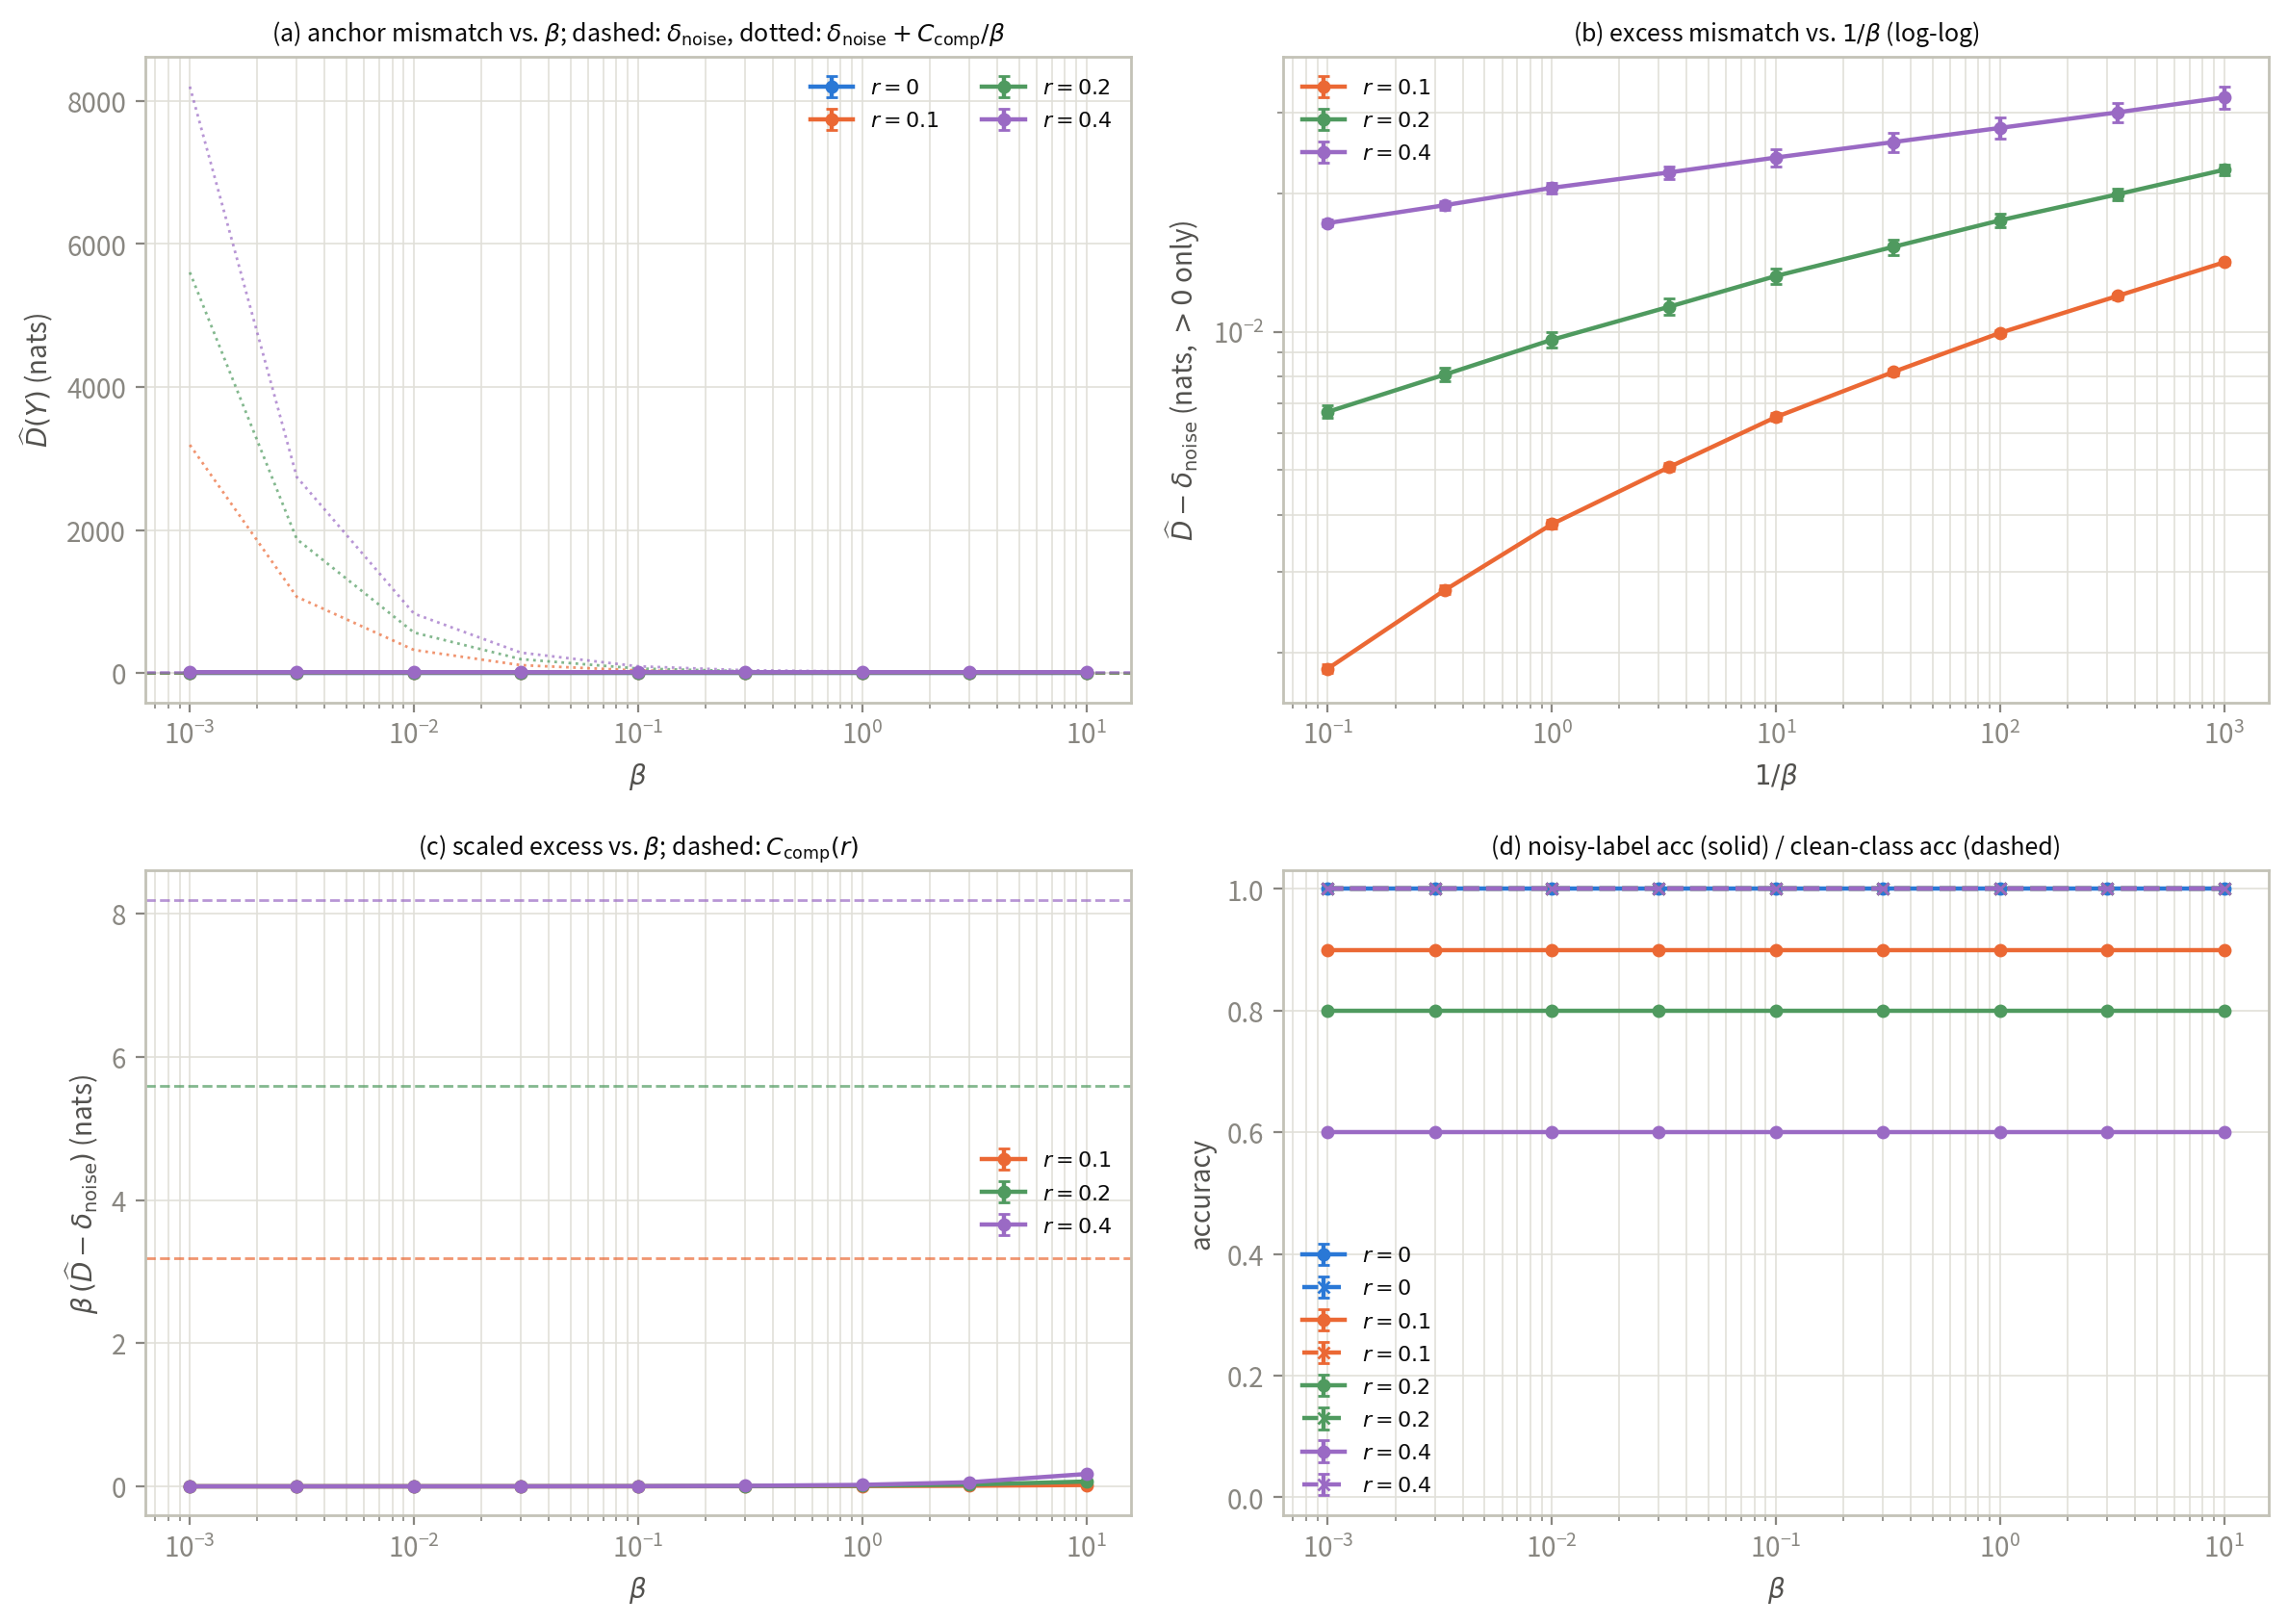
\includegraphics[width=\linewidth]{figures/fig_noisy_alignment.png}
\caption{Controlled illustration of approximate realizability. (a) Anchor mismatch
$\widehat D$ against $\beta$; dashed lines are the analytic ambiguity floors and dotted
lines the comparator references
$\delta_{\mathrm{noise}}+C_{\mathrm{comp}}/\beta$. (b) Excess mismatch against
$1/\beta$. (c) Scaled excess $\beta(\widehat D-\delta_{\mathrm{noise}})$ against the
comparator risks. (d) Accuracy on the corrupted label (solid) and clean class (dashed).
Points are means and error bars are standard deviations over five seeds.}
\label{fig:controlled-noisy-alignment}
\end{figure*}

Fixed-posterior-variance and trainable-polar-frame controls reproduce the same analytic
floors (Appendix~\ref{app:noisy-alignment-sensitivity}). A sampled-label version exposes
the expected finite-sample and optimization sensitivity: six large-$\beta$
configurations fail the comparator-objective gate and are marked rather than counted as
counterexamples. This experiment is a controlled illustration of the ambiguity term and
the comparator inequality. It neither estimates the comparator floor on a real dataset
nor turns the benchmark accuracy comparison into a theorem test.

\subsection{Main results}
\label{sec:main-results}

% 主结果表：由 paper/make_table.py 从 tune_results/*.html 自动生成，请勿手改。
% 分类任务为测试 Acc（%）、回归任务为测试 R²；均为 5 次运行均值（不含标准差）。
% 每格取该模型在 β / anchor-scale 调参网格上的最优配置（tune_results 各表绿色高亮行），
% 每行（数据集）的最优指标加粗、次优（并列次优全部）加下划线；表尾两行统计各方法跨行的平均排名（越低越好）与最优/并列最优次数。
\begin{table*}[t]
\centering
\caption{Test accuracy (\%) on classification tasks and test $R^2$ on regression tasks (mean over 5 runs). Each entry reports the best configuration over the tuned $\beta$ (and anchor-scale) grid; the best entry per dataset is bolded.}
\label{tab:main_result}
\small
{
\setlength{\tabcolsep}{2pt}
\begin{tabular}{llcccccc|cc}
\hline
Dataset & Backbone & Base & VIB & SVIB & NIB & CEB & DVCCA & GPB & OPB-L \\
\hline
MNIST & MLP & 98.33 & 98.28 & 98.15 & 98.27 & \underline{98.43} & 98.24 & \textbf{98.54} & \underline{98.43} \\
MNIST & CNN & 99.13 & 99.28 & 99.23 & 99.22 & 99.30 & 99.29 & \textbf{99.32} & \underline{99.31} \\
ImageNet-100 & MLP & 83.12 & 82.84 & 83.02 & 82.35 & 82.77 & 82.99 & \textbf{84.40} & \underline{84.01} \\
ImageNet-100 & CNN & 83.40 & 82.94 & 83.11 & 82.91 & 82.97 & 83.21 & \textbf{86.08} & \underline{84.88} \\
Cora & GCN & 87.68 & 86.83 & 86.46 & 86.35 & 86.27 & 86.90 & \textbf{88.12} & \underline{87.86} \\
IMDb & RNN & 84.85 & 85.50 & 85.99 & 86.14 & 85.55 & 85.69 & \underline{86.84} & \textbf{86.99} \\
AG News & RNN & \textbf{92.94} & 92.72 & 92.86 & 92.91 & 92.83 & 92.78 & 92.87 & \underline{92.92} \\
\hline\hline
Cal. Housing & MLP & 0.7618 & \underline{0.7901} & 0.7897 & 0.7862 & 0.7894 & 0.7878 & 0.7895 & \textbf{0.7914} \\
STS-B & RNN & \textbf{0.2899} & 0.2719 & 0.2697 & 0.2417 & 0.2668 & 0.2713 & \underline{0.2762} & 0.2755 \\
ZINC & GCN & \textbf{0.6348} & 0.6339 & 0.6325 & 0.6178 & 0.6257 & 0.6294 & \underline{0.6344} & 0.6323 \\
AgeDB & MLP & 0.2180 & 0.3173 & \underline{0.3385} & 0.2710 & 0.3317 & 0.3180 & \textbf{0.3536} & 0.3320 \\
AgeDB & CNN & 0.3914 & 0.3342 & 0.3323 & 0.3337 & 0.3882 & 0.3205 & \textbf{0.4700} & \underline{0.4388} \\
\hline
\multicolumn{2}{l}{Mean rank (of 12)} & 4.25 & 5.25 & 5.00 & 6.50 & 5.46 & 5.50 & 1.75 & 2.29 \\
\multicolumn{2}{l}{Best or tied-best (of 12)} & 3 & 0 & 0 & 0 & 0 & 0 & 7 & 2 \\
\hline
\end{tabular}
}
\end{table*}


Table~\ref{tab:main_result} reports test accuracy (classification) and test $R^2$
(regression), averaged over runs, for each method's best configuration; bold
marks the best mean per row and underline the second best, and the vertical rule
separates GPB and its free-head ablation GPB-L from the baselines. NCBD
(classification settings only) and AdaCap (regression settings only) are external
non-IB baselines under the same protocol; dashes mark the settings where a method
does not apply. Statistical claims (best vs.\ tied) follow the paired-difference
confidence intervals of Appendix~\ref{app:main-ci}.
Standard deviations are omitted for width and are reported in
Appendix~\ref{app:main-std}. Three
observations.

\emph{The constructed geometry is free, and it usually pays.} GPB is best or
tied-best in $7$ of $12$ settings with mean rank $1.83$, against $4.83$ for the plain
backbone and $5.50$--$7.00$ for the variational baselines, none of which is ever
best; among the external baselines NCBD never wins and AdaCap wins once (ZINC).
By the paired bootstrap $95\%$ CIs (Appendix~\ref{app:main-ci}), the GPB--CEB
difference is significantly positive in $8$ of $12$ settings and within the
non-inferiority margin in three more; only on STS-B does the interval overlap zero
beyond the margin ($[-0.009, +0.025]$), so no setting shows a significant CEB
advantage. GPB dominates CEB by mean in all $12$ settings and is best among all
methods on seven rows.
The gains concentrate where the label structure is rich or supervision is scarce:
$+3.1$ accuracy over CEB on ImageNet-100 with the CNN backbone ($86.1$ vs.\ $83.0$),
$+1.9$ on Cora, and $+0.08$ $R^2$ on AgeDB over the plain CNN ($0.470$ vs.\ $0.388$).
On saturated settings (MNIST) the margin is small but consistent, and on the two
rows where the plain backbone remains best (STS-B, AG News) the gap is
marginal ($\le 0.03$): the geometry is neutral there rather than harmful. On
ZINC every bottleneck method trails the plain backbone, but the closed-form
AdaCap readout edges it out ($0.677$ vs.\ $0.635$ $R^2$), the one setting where
any comparison method significantly beats GPB (see below).

\emph{Prediction does not require the free head.} GPB-L, the free linear head on the
same geometric prior, is best or tied-best in $2$ of $12$ settings (mean rank
$2.54$), and the GPB--GPB-L gap is within $0.4$ accuracy or $R^2$ points in $11$ of
$12$ settings (the exception is ImageNet-100 CNN, $1.2$ points): the zero-parameter
anchor-energy classifier --- whose weights are the frame itself --- reaches the
accuracy of a freely trained head in almost all settings, so the degrees of freedom
removed by construction are not required for prediction, as claimed in the
introduction. The three settings where GPB-L edges out GPB by mean (IMDb, AG News,
Cal.\ Housing) do so with paired CIs overlapping zero, confirming that the tie
does not inflate the numbers. On the five
regression rows the tied projection head of EPB wins or matches the free
regression head in four (the exception is Cal.\ Housing by $0.002$).

\emph{The tie regularizes the high-cardinality and low-data regimes.} The two
settings with the largest GPB margins (ImageNet-100, with $K = 100$, and AgeDB, a
small, high-variance regression task) are exactly those where an unconstrained
classifier can overfit its own scale or the scarce supervision: fixing the
prediction rule to the prior's geometry removes both escape routes, consistent with
the fixed-scale condition under which the aligned surrogate of
Proposition~\ref{prop:opb-sweep} has a unique interior optimum per $\beta$.

\emph{External baselines do not close the gap.} By the paired CIs
(Appendix~\ref{app:main-ci}), GPB beats NCBD significantly on $6$ of $7$
classification settings; the exception is IMDb ($+0.2$ points, CI $[-0.5,+0.7]$
crossing zero), where the GPB margin is within noise. The largest margin is
ImageNet-100 with the CNN backbone ($+5.5$ points, CI $[+4.3,+6.9]$). On the
regression side GPB beats AdaCap significantly on Cal.\ Housing ($+0.014$ $R^2$)
and STS-B ($+0.115$ $R^2$), and the AgeDB intervals straddle zero (the CNN one
within the non-inferiority margin). The single reversal is ZINC, where AdaCap is
the only method with a significant advantage over GPB ($-0.043$ $R^2$, CI
$[-0.046,-0.041]$): its ridge readout, refit on the training set at evaluation
time, exploits the low-dimensional regression structure of molecular-graph labels
without any compression objective. Neither external baseline performs
information-bottleneck compression, so their sweeps exercise the same data but a
different axis of the comparison.

\subsection{Attribution ablations: what drives the gain?}
\label{sec:ablation}

The GPB construction bundles three mechanisms --- the orthogonal/isometric
geometry, the fixed anchor scale, and the tied geometric readout --- with the
IB objective itself, and the main table alone cannot attribute the gain among
them. This section switches each factor off separately. All variants are
trained under the protocol of Section~\ref{sec:setup} (same $\beta$ and anchor
grids, five seeds, per-variant configuration selection) on the three settings
of the mechanism analysis, and the reference models (Base, CEB, GPB, GPB-L)
are re-trained in the same batch so every comparison is paired by seed.

\paragraph{The ablation ladder.} \emph{NCM-learn} removes the bottleneck
entirely: $z = \mu_\phi(x)$ is deterministic, prediction is the energy rule
$\mathrm{logit}_k = -\|z - m_k\|^2/2$ on trainable prototypes $m_k$, and there is no
posterior and no KL. \emph{NCM-ortho} fixes the prototypes to the orthogonal
frame $a\,e_k$: fixed geometry, still no IB. \emph{CEB-energy} and
\emph{CEB-tied} mount the same energy readout (resp.\ the tied projection) on
CEB's trainable free reference: free geometry, free scale, restricted
readout, with IB. \emph{OPB-FS} and \emph{EPB-FS} keep the orthogonal frame
and the energy (resp.\ tied) readout but make the anchor radius learnable ---
per-class scales $s_k$, or a scalar $\rho$ --- initialized at the anchor
scale, so only the fixed scale is switched off. Together with Base, CEB,
GPB-L and GPB the ladder switches each factor independently:
geometry (CEB-energy vs.\ OPB-FS), scale (OPB-FS vs.\ GPB), readout
(GPB-L vs.\ GPB; CEB vs.\ CEB-energy), and the IB term itself
(NCM-ortho vs.\ GPB).

\begin{table}[t]
\centering
\small
\caption{Attribution ablation: best-configuration test metrics (mean $\pm$ std
over seeds). Configurations are selected by the mean validation metric
(accuracy on MNIST and ImageNet-100), applied identically to
every variant, so all comparisons remain paired by seed and the test split is
never touched by selection. One OPB-FS configuration (ImageNet-100,
$\beta = 10^{-4}$, $a = 1$) diverged during training (free scales grow without
penalty at negligible $\beta$) and is excluded.}
\label{tab:ablation}
\begin{tabular}{l c c}
\hline
variant & MNIST (Acc \%) & ImageNet-100 (Acc \%) \\
\hline
Base & $98.33 \pm 0.12$ & $83.12 \pm 0.14$ \\
NCM-learn & $98.17 \pm 0.17$ & $82.17 \pm 0.36$ \\
NCM-ortho & $98.11 \pm 0.12$ & $82.33 \pm 0.60$ \\
CEB & $98.43 \pm 0.08$ & $82.78 \pm 0.22$ \\
CEB-energy & $98.22 \pm 0.10$ & $81.59 \pm 0.21$ \\
GPB-L & $98.43 \pm 0.07$ & $83.40 \pm 0.67$ \\
GPB & $98.44 \pm 0.08$ & $84.22 \pm 0.15$ \\
OPB-RV & $98.34 \pm 0.04$ & $83.38 \pm 0.52$ \\
OPB-FS & $98.54 \pm 0.03$ & $84.26 \pm 0.18$ \\
\hline
\end{tabular}
\end{table}


\begin{table}[t]
\centering
\small
\setlength{\tabcolsep}{3pt}
\caption{Factor-wise paired differences (accuracy points on MNIST and
ImageNet-100; $95\%$ bootstrap percentile CIs; positive values favor the
first term).}
\label{tab:ablation-ci}
\begin{tabular}{l l c c}
\hline
factor & comparison & MNIST & ImageNet-100 \\
\hline
readout & GPB $-$ GPB-L & $+0.02$ [$_{-0.05}$, $_{0.08}$] & $+0.82$ [$_{0.34}$, $_{1.17}$] \\
readout (free geometry) & CEB-energy $-$ CEB & $-0.21$ [$_{-0.30}$, $_{-0.12}$] & $-1.19$ [$_{-1.50}$, $_{-0.96}$] \\
geometry & GPB $-$ CEB-energy & $+0.23$ [$_{0.10}$, $_{0.36}$] & $+2.63$ [$_{2.41}$, $_{2.88}$] \\
frame trainability & GPB $-$ OPB-RV & $+0.10$ [$_{0.05}$, $_{0.15}$] & $+0.83$ [$_{0.29}$, $_{1.19}$] \\
IB increment & GPB $-$ NCM-ortho & $+0.34$ [$_{0.22}$, $_{0.45}$] & $+1.89$ [$_{1.41}$, $_{2.36}$] \\
prototype structure & NCM-ortho $-$ NCM-learn & $-0.06$ [$_{-0.20}$, $_{0.11}$] & $+0.16$ [$_{-0.49}$, $_{0.82}$] \\
prototype readout alone & NCM-learn $-$ Base & $-0.16$ [$_{-0.28}$, $_{-0.05}$] & $-0.96$ [$_{-1.30}$, $_{-0.69}$] \\
\hline
\end{tabular}
\end{table}


\paragraph{Where the gain comes from.} Table~\ref{tab:ablation} reports the
best configuration of each variant and Table~\ref{tab:ablation-ci} the
factor-wise paired differences. On ImageNet-100 the decomposition is clean:
the geometry contributes $+2.67$ points (OPB-FS $-$ CEB-energy,
CI $[2.45, 2.92]$), the IB term $+1.89$ (GPB $-$ NCM-ortho,
$[1.41, 2.36]$), and the restricted readout $+0.82$ (GPB $-$ GPB-L,
$[0.34, 1.17]$), while the fixed scale is neutral ($-0.04$,
$[-0.07, -0.01]$). The readout effect flips sign on the free-geometry side,
where the energy head costs CEB $1.19$ points ($[-1.50, -0.96]$): the
restricted readout pays only on the constructed geometry. Most informative is
the negative result on the prototype readout alone: NCM-learn trails the
plain backbone by $0.96$ points ($[-1.30, -0.69]$), so the gain is not a
nearest-class-mean effect in disguise --- the prototypes need the IB
objective and the orthogonal geometry to carry prediction. On MNIST the same
ordering holds with small margins (geometry $+0.32$, IB $+0.34$, scale
$+0.09$, readout $\approx 0$), and on Cal.\ Housing every EPB variant ties
within $0.01$ $R^2$, consistent with the flat EPB plateaus of
Section~\ref{sec:sweep}. The conclusion is that the orthogonal geometry is
the primary driver of the ImageNet-100 gain, and it acts \emph{within} the IB
framework: geometry, IB, and readout each contribute positively, in that
order, and none of the bundled mechanisms is doing the work alone.

\subsection{Compression--accuracy and the KL certificate over $\beta$}
\label{sec:sweep}

The main table selects the best $(\beta, a)$ per method; the figures below report
the compression--accuracy trade-off on one classification and one regression
setting (ImageNet-100 and Cal. Housing, both with the MLP backbone). Each setting
has two companion panels over the same $\beta$ grid: the task metric against
$\beta$ (panels a--b), and the realized test-set $\E[\KL]$ --- the certificate
itself --- against $\beta$ (panels c--d). The certificate panels are what make a
$\beta$-matched sweep interpretable: the two methods reach different compressions
at the same $\beta$ --- on Housing at $\beta = 0.1$, CEB sits at
$\E[\KL] \approx 0.09$ while EPB ($\rho = 12$) is at $\approx 0.27$ --- so the
compression each point actually achieves is read off directly rather than
assumed from $\beta$. No points are omitted: collapsed references and variance
explosions are visible at the extremes of the sweep.

\begin{figure*}[t]
\centering
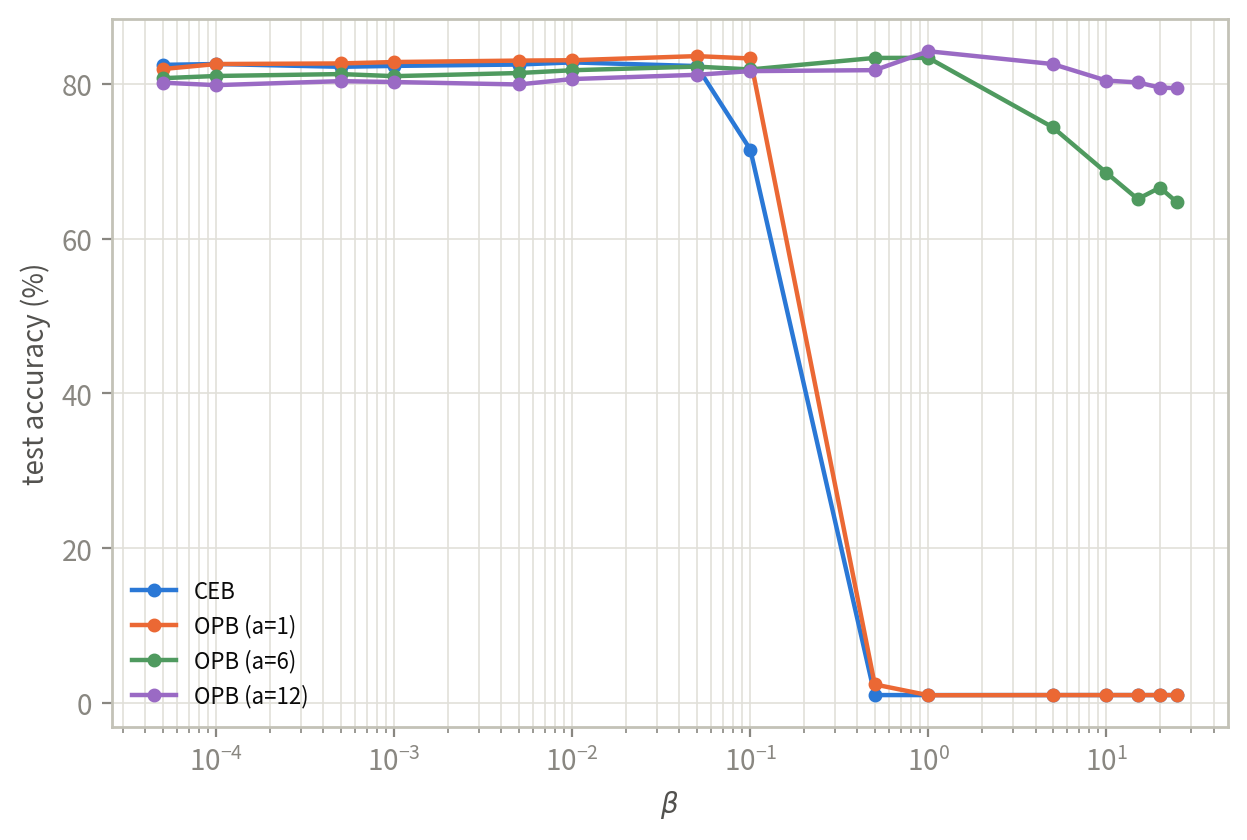
\includegraphics[width=0.48\linewidth]{figures/fig_beta_acc_imagenet100.png}\hfill
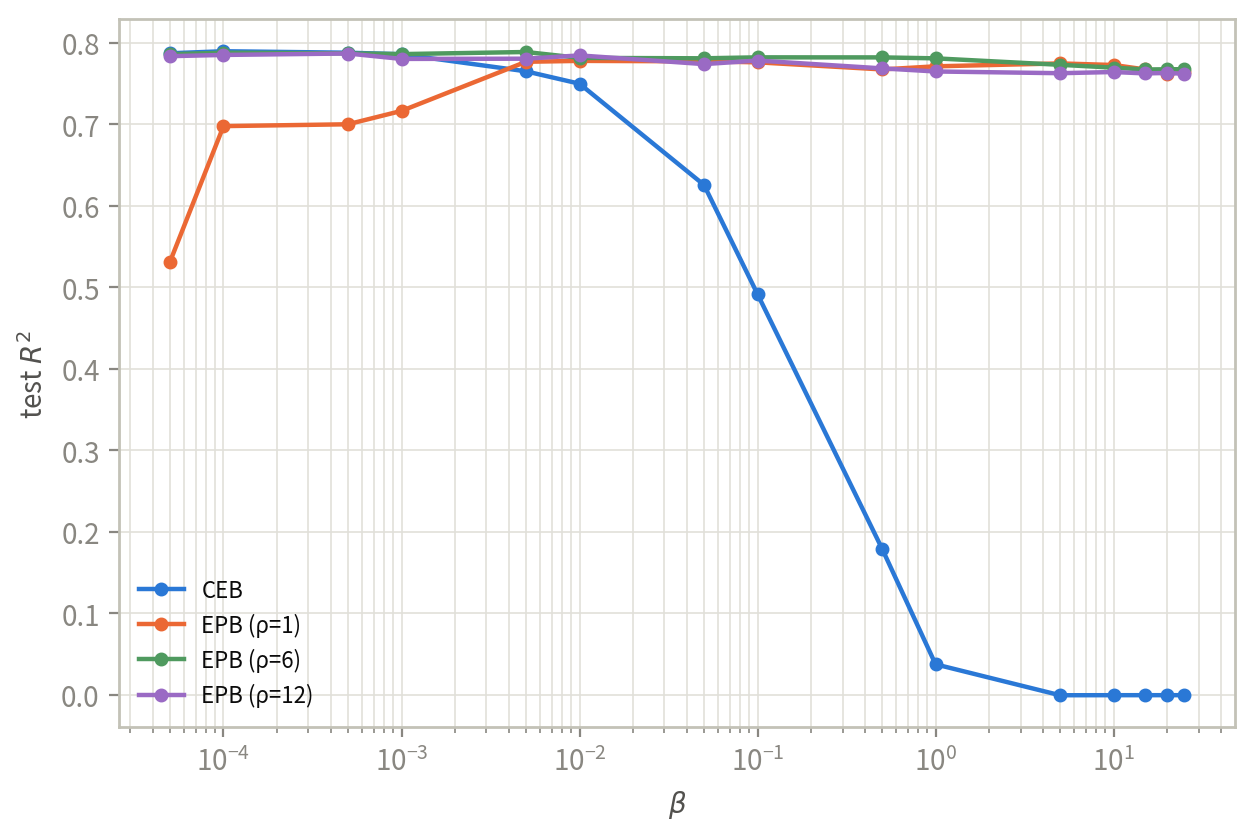
\includegraphics[width=0.48\linewidth]{figures/fig_beta_acc_housing.png}\\[2pt]
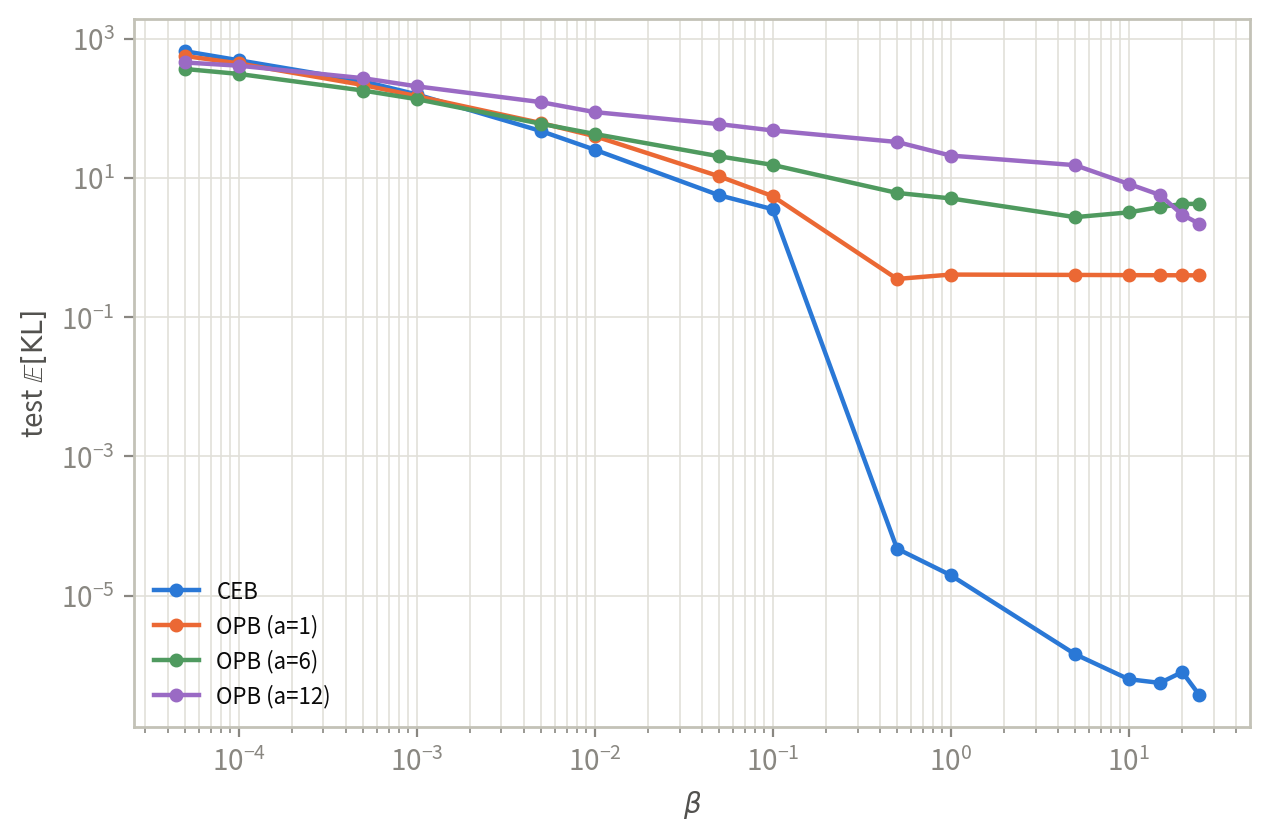
\includegraphics[width=0.48\linewidth]{figures/fig_beta_kl_imagenet100.png}\hfill
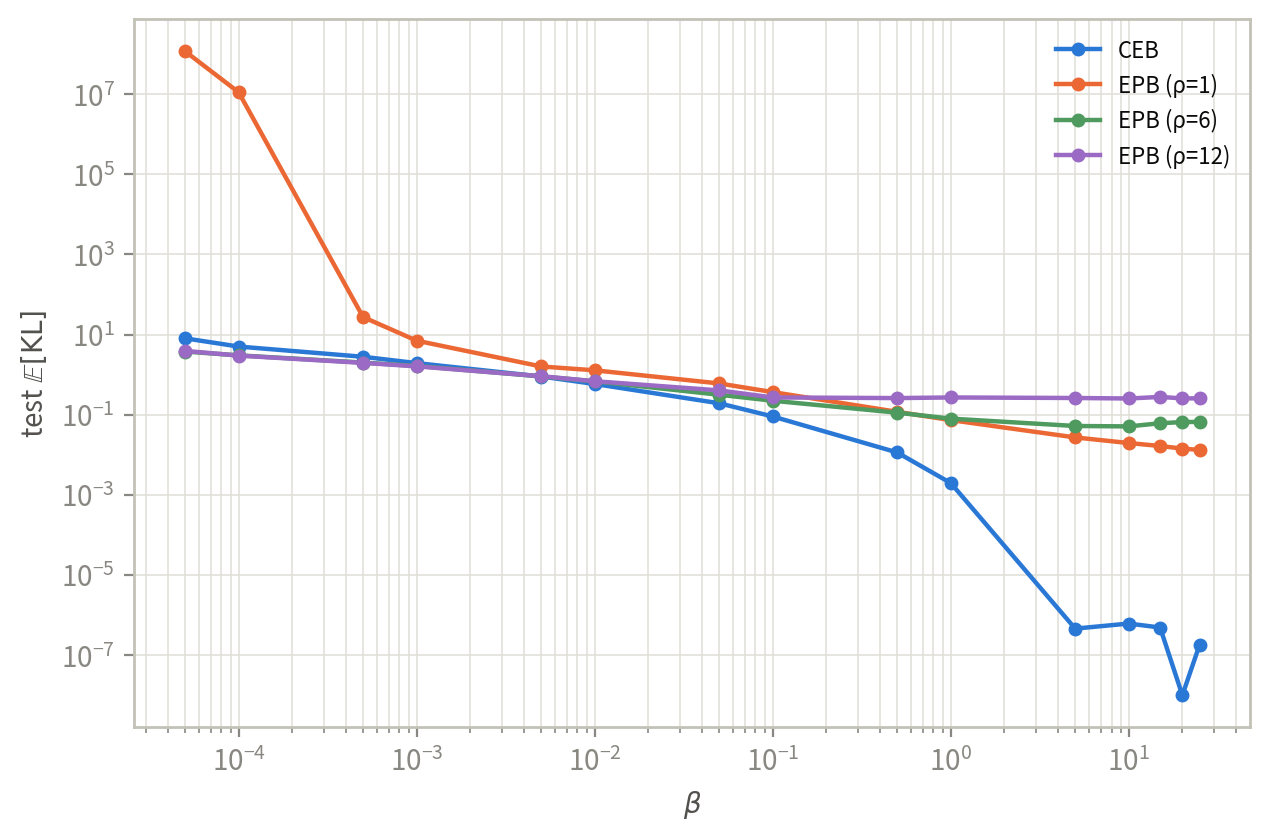
\includegraphics[width=0.48\linewidth]{figures/fig_beta_kl_housing.png}
\caption{Compression--accuracy and the realized certificate over $\beta$ (log
scale), $\beta \in \{5{\cdot}10^{-5}, \dots, 25\}$; CEB one curve per panel, GPB
three ($a$ on classification, $\rho$ on regression, both $\in \{1, 6, 12\}$).
(a)--(b) Test accuracy (\%) on ImageNet-100 (MLP) and test $R^2$ on Cal.\
Housing (MLP) against $\beta$: OPB with $a = 12$ holds the plateau out to
$\beta = 25$ while CEB and OPB ($a = 1$) collapse. (c)--(d) The realized
test-set $\E[\KL]$ against $\beta$ (log scale) for the same runs: CEB's
certificate collapses with its reference, EPB ($\rho = 1$) explodes near
$\beta = 5{\cdot}10^{-5}$, and the larger anchors keep $\E[\KL]$ in a stable
band.}
\label{fig:compression}
\end{figure*}

Figure~\ref{fig:compression}
exhibits the two roles of the anchor scale across the $\beta$ sweep, with panels
(c)--(d) translating each point into its realized compression.
\emph{(i) Without a scale, the reference collapses.} On ImageNet-100, CEB's
accuracy erodes to $71.5\%$ at $\beta = 0.1$ ($\E[\KL] \approx 3.6$) and its
reference escapes entirely at $\beta \ge 0.5$ ($\E[\KL] \to 0$ with accuracy at
chance, panel c); OPB at $a = 1$ survives one grid step longer ($83.3\%$ at
$\beta = 0.1$) and collapses at the same end of the sweep. OPB ($a = 6$) holds
accuracy above $74\%$ out to $\beta = 5$ and falls to $64.7\%$ at $\beta = 25$.
On Housing, CEB drops to $R^2 = 0.49$ at $\beta = 0.1$ and below $0.1$
by $\beta \ge 0.5$, while every EPB curve keeps $R^2 \ge 0.76$ out to
$\beta = 25$. Orthogonality alone therefore does not prevent the collapse: the
frame is fixed up to rotation, but the anchor-energy classifier's margin is
$a^2/\tau^2$ (Proposition~\ref{prop:opb-energy}), and at $a = 1$ that margin is
too small to carry a solution at strong compression. \emph{(ii) The anchor scale
controls where the collapse sets in, and at matched compression the geometry pays
or ties.} On ImageNet-100, OPB ($a = 12$) attains $84.2\%$ at $\beta = 1$
($\E[\KL] \approx 21$), above CEB's best point anywhere on its sweep
($82.8\%$ at $\beta = 10^{-2}$), and still $79.4\%$ at $\beta = 25$
($\E[\KL] \approx 2.2$); on Housing the four curves peak within half a point
(CEB $0.789$, EPB $0.786$--$0.789$), but only EPB retains its peak into the
strong-compression regime: the plateau is the flat EPB segment where $R^2$ stays
above $0.76$ from $\beta = 0.1$ out to $\beta = 25$ while the certificate keeps
shrinking.

A visible cost remains in the weak-compression regime: on ImageNet-100 at
$\beta = 10^{-4}$ ($\E[\KL] \gtrsim 300$), OPB trails CEB by one to three points
($a = 6$: $81.0$ vs.\ $82.6$; $a = 12$: $79.8$ vs.\ $82.6$): the price of the
fixed-scale energy rule when compression is weak. On Housing the same regime
shows EPB ($\rho = 1$) dipping to $R^2 = 0.53$ at $\beta = 5{\cdot}10^{-5}$,
where its certificate explodes to $\approx 10^{8}$ (panel d): with a unit axis
and negligible $\beta$ the off-axis variance is unconstrained. The construction
pays for itself in the strong-compression regime, where CEB is at chance.

These curves are empirical compression diagnostics, not a test of the zero-floor
rate. For every benchmark distribution, Theorem~\ref{prop:pgib-alignment} bounds
anchor mismatch relative to any feasible comparator, but its ambiguity and
approximation floor is unknown. Only in the deterministic exactly realizable special
case does Corollary~\ref{cor:pgib-exact-alignment} reduce the bound to
$(\ln K+\varepsilon)/\beta$. At exact alignment, the Gaussian mixture's accuracy is
governed by the scale-to-noise ratio $a/\tau$ (the nearest-anchor error probability is
$\Phi(-a/(\sqrt{2}\tau))$; appendix). For the benchmark runs, the realized KL and
geometry are therefore inspected directly. With the classifier scale
fixed at $a/\tau^2$ by construction, the only remaining lever at full compression is
$a$ itself: the anchor scale converts the compression knob from a collapse dial into
a plateau dial. The KL decomposition shows the two channels at work: OPB's $\E[\KL]$ is
dominated by the mean-mismatch term (anchor displacement; $a = 12$, $\beta = 1$:
$20.6$ mean vs.\ $0.36$ variance), while CEB's reference absorbs compression by
shrinking both terms toward zero: the reference chases the posterior, exactly the
degeneracy the constructed geometry excludes
(Lemma~\ref{lem:opb-kl-decomposition}). This decomposition motivates the direct
mismatch diagnostics of Section~\ref{sec:direct-mismatch}; it does not by itself
verify the comparator bound. The geometry transfer is characterized by the
mismatch-dependent separation statement (Proposition~\ref{prop:pgib-separation}) and
the fixed-scale condition of
Proposition~\ref{prop:opb-sweep}; consistent with that proposition's scope, we do
not claim that the map $\beta \mapsto$ accuracy is monotone, only that the
constructed scale keeps the plateau from collapsing.

\subsection{Information-plane analysis}
\label{sec:info-plane}
% =====================================================================

The certificate tells us \emph{which} gap the KL measures; the panels below
inspect \emph{what} each method actually discards. On every sweep checkpoint we
estimate the three quantities of the canonical information plane
(Fig.~\ref{fig:info-plane}): $I(X;Z)$ by the InfoNCE lower bound
\citep{oord2018representation} ($\log B - \mathcal{L}_{\mathrm{NCE}}$,
$B = 4096$, one critic per run trained on the training split, the bound read
off the test split with $z \sim q(z|x)$); $I(Y;Z)$ by the classification lower
bound $H(Y) - \CE(\mathrm{logits})$; and the residual $I(X;Z|Y)$ as the
difference of the two --- a heuristic, not a
bound. The true residual is nonnegative by the data-processing inequality;
negative plotted values mean the estimators, not the theory, gave way, and they
occur exactly where the InfoNCE bound fails (see the caveats below). Consistent
with Remark~\ref{rem:opb-scope}, this section reports estimator-level
observations on the sweep checkpoints and claims nothing about the exact plane.

\begin{figure*}[t]
\centering
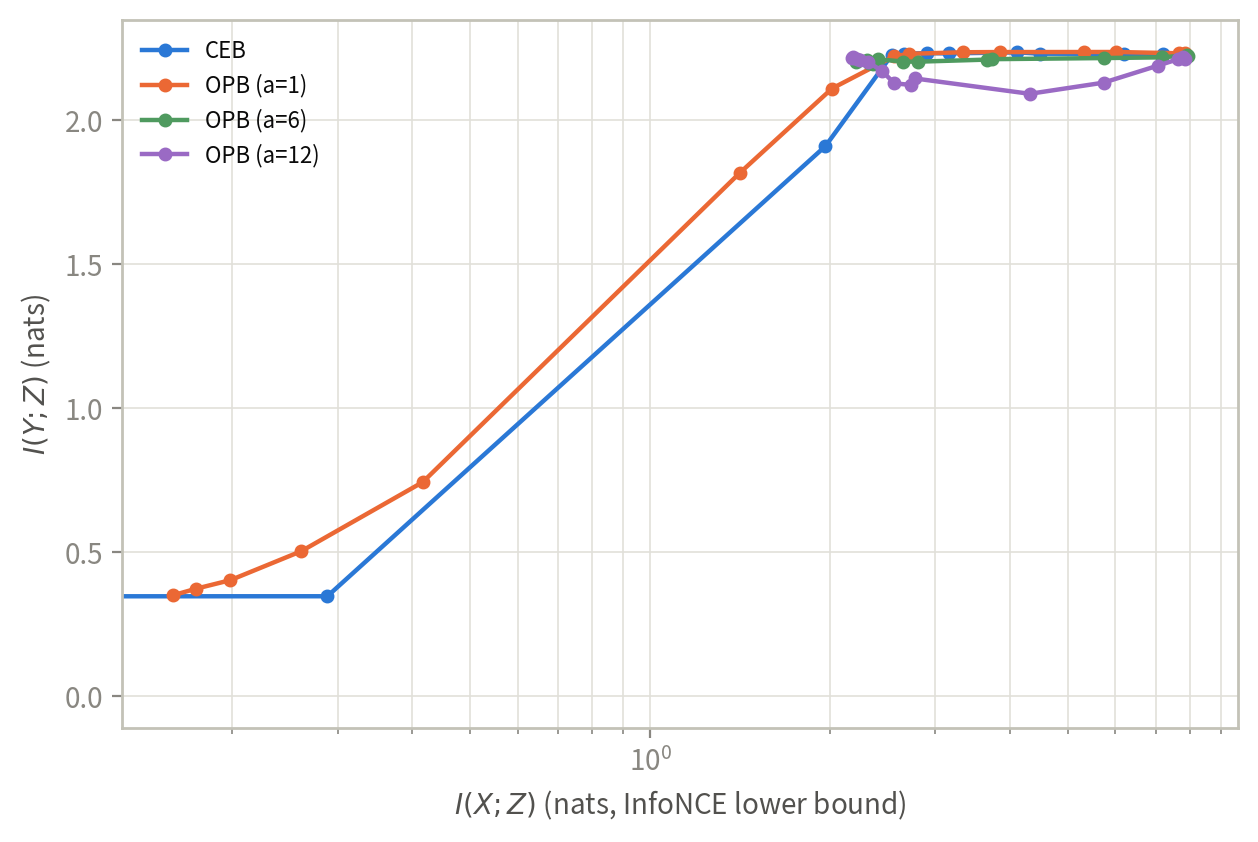
\includegraphics[width=0.48\linewidth]{figures/fig_info_plane_mnist.png}\hfill
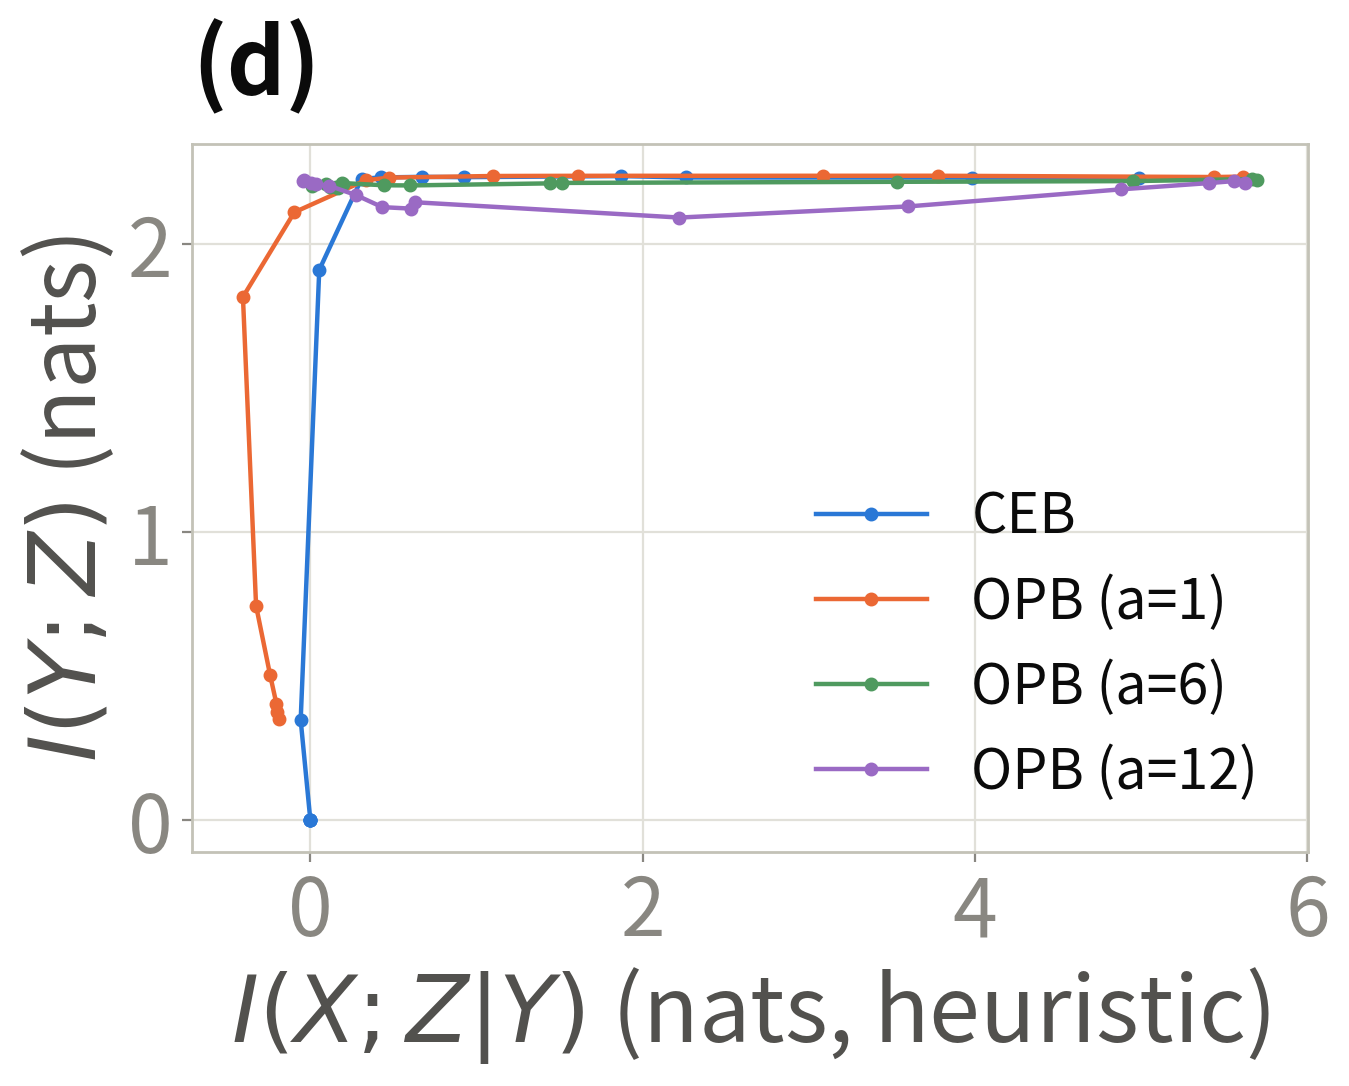
\includegraphics[width=0.48\linewidth]{figures/fig_certificate_plane_mnist.png}
\caption{Information plane (a) and certificate plane (b) on MNIST over the
$\beta$ sweep, five runs per point, lines connect $\beta$ in ascending order;
$x$ is log-scaled in (a), and the certificate axis in (b) switches to a linear
scale wherever the estimated residual turns negative (OPB $a = 1$ at
$\beta \ge 5$, see text). CEB one curve per panel; OPB three
($a \in \{1, 6, 12\}$). CEB follows the classic corner --- compression and task
information drop together past a critical $\beta = 0.5$ with bimodal runs ---
and collapses to chance by $\beta = 1$; OPB ($a = 6$, $12$) keeps accuracy flat
out to $\beta = 25$ with $I(X;Z)$ saturating at $\approx 2.2$--$2.4$ nat,
essentially all of it task-relevant (certificate $\approx 0$). The Cal.\
Housing panels are deferred to Fig.~\ref{fig:info-plane-extra} in the
appendix.}
\label{fig:info-plane}
\end{figure*}

\emph{(i) The corner is sharp.} On MNIST, CEB moves from $I(X;Z) = 2.53$ at
$98.2\%$ ($\beta = 0.1$) to $1.96$ at $86.0\%$ ($\beta = 0.5$) to $0.29$ at
$26.8\%$ ($\beta = 1$), and to chance beyond. The $\beta = 0.5$ point is a
critical point rather than a midpoint: the per-seed accuracy is bimodal
($86.0 \pm 22.5\%$; one run collapses to $41\%$ while four sit at
$96.5$--$97.8\%$). The two axes fall together --- the reference absorbs the
compression by absorbing the task information.

\emph{(ii) The plateau has a floor at the task information.} OPB
($a = 6$, $12$) keeps MNIST accuracy at $98.1$--$98.6\%$ for every $\beta$ up
to $25$; $I(X;Z)$ saturates at $2.2$--$2.4$ nat while $I(Y;Z)$ stays at
$\approx 2.2$ (against $H(Y) = \ln 10 \approx 2.30$), and the certificate sits
at $\approx 0$ ($a = 12$, $\beta = 15$: $0.00 \pm 0.21$; $a = 6$,
$\beta = 5$: $0.09$). The floor is the data-processing inequality made
visible: at full compression the frame leaves room for exactly the
task-relevant information and nothing else.

\emph{(iii) At matched compression the geometry keeps more of the task.}
Table~\ref{tab:info-plane-matched} pairs each CEB point with the OPB
configuration of nearest estimated $I(X;Z)$. At $\approx 2.0$ nat, CEB
($\beta = 0.5$) retains $86.0\%$ while OPB ($a = 1$, $\beta = 0.5$) retains
$97.8\%$; at $\approx 2.5$ nat ($\beta = 0.1$) the two tie ($98.2\%$ vs.\
$98.1\%$) --- the geometry pays nothing where compression is mild and carries
the task where it is not.

\begin{table}[t]
\centering
\small
\begin{tabular}{l c c c c c}
\hline
& \multicolumn{2}{c}{CEB} & \multicolumn{3}{c}{OPB (nearest $I(X;Z)$)} \\
\cline{2-3} \cline{4-6}
Setting & $I(X;Z)$ & Acc & config & $I(X;Z)$ & Acc \\
\hline
MNIST, $\beta = 0.1$ & $2.53 \pm 0.03$ & $98.2 \pm 0.1$ & $a = 1$, $\beta = 0.1$ & $2.55 \pm 0.01$ & $98.1 \pm 0.1$ \\
MNIST, $\beta = 0.5$ & $1.96 \pm 0.53$ & $86.0 \pm 22.5$ & $a = 1$, $\beta = 0.5$ & $2.01 \pm 0.03$ & $97.8 \pm 0.1$ \\
\hline
\end{tabular}
\caption{Matched-compression comparison on MNIST: each CEB checkpoint is
paired with the OPB configuration of nearest estimated $I(X;Z)$ (nats;
mean $\pm$ std over five runs). At matched compression the geometric prior
retains strictly more of the task; the CEB $\beta = 0.5$ entry is the
bimodal critical point of the collapse transition (individual runs at
$97\%$ or $41\%$).}
\label{tab:info-plane-matched}
\end{table}

\emph{Estimator caveat.} One region must be read with care, and it is not used
for any claim above: OPB ($a = 1$) at
$\beta \ge 5$. There the plotted estimates collapse ($I(X;Z) \le 0.42$ nat)
while accuracy stays $97.6$--$97.8\%$; by Fano's inequality the $2.3\%$ error
alone requires $I(Y;Z) \ge H(Y) - h(0.023) - 0.023 \ln 9 \approx 2.1$ nat, so
the leftward spur is a bound failure, not compression: $z$ quantizes onto the
ten anchors, near-duplicate positives saturate the InfoNCE objective
\citep{poole2019variational}, and overconfident errors inflate the
cross-entropy.

\subsection{Adversarial robustness}
\label{sec:robustness}

We evaluate robustness to white-box attacks following the CEB paper's
\emph{targeted} variant (its Figure~4, bottom panels): targeted projected
gradient descent (PGD, $20$ steps, step size $2.5\varepsilon/\mathrm{steps}$,
random start) toward a single class, with success measured as the fraction of
originally correct predictions flipped to that class. The target is digit
$0$, the most distinctive MNIST class (the analogue of Fashion-MNIST
``trouser''), so that class confusion does not masquerade as robustness.
$\varepsilon$ is defined in the normalized pixel space (MNIST mean/std); we
attack $1{,}000$ test images and report the mean and standard deviation over
runs. All stochastic models are attacked and evaluated on their
\emph{stochastic} path: each PGD step averages gradients over $10$ samples of
$z \sim q_\phi(z|x)$ (expectation over transformation), and every prediction is
the majority class under $10$ MC samples. We use $\varepsilon_\infty = 0.3$ and
$\varepsilon_2 = 6.0$ --- the smallest $L_2$ budget we tested at which the
targeted attack engages the decision boundaries at all (at $2.0$ it cannot
reach the target region from any other class and sits at a near-zero floor for
every model). Every curve is drawn only over the $\beta$ values at which the model's
clean accuracy clears a shared $90\%$ failure threshold under the same
stochastic protocol: below it a configuration is counted as failed, and a
failed model's near-zero attack success is not robustness. The threshold
binds CEB at $\beta \le 0.1$ (beyond, the reference collapses to chance) and
OPB ($a = 1$) at $\beta \le 1$ (beyond, its posterior retains substantial
stochastic variance while its means pin to the radius-$1$ anchors, and the
MC-sampled predictions fall to $0.59$--$0.84$ clean accuracy even though the
deterministic path keeps $0.98$); OPB ($a = 6$, $12$) clears the threshold
across the full grid.

\begin{figure*}[t]
\centering
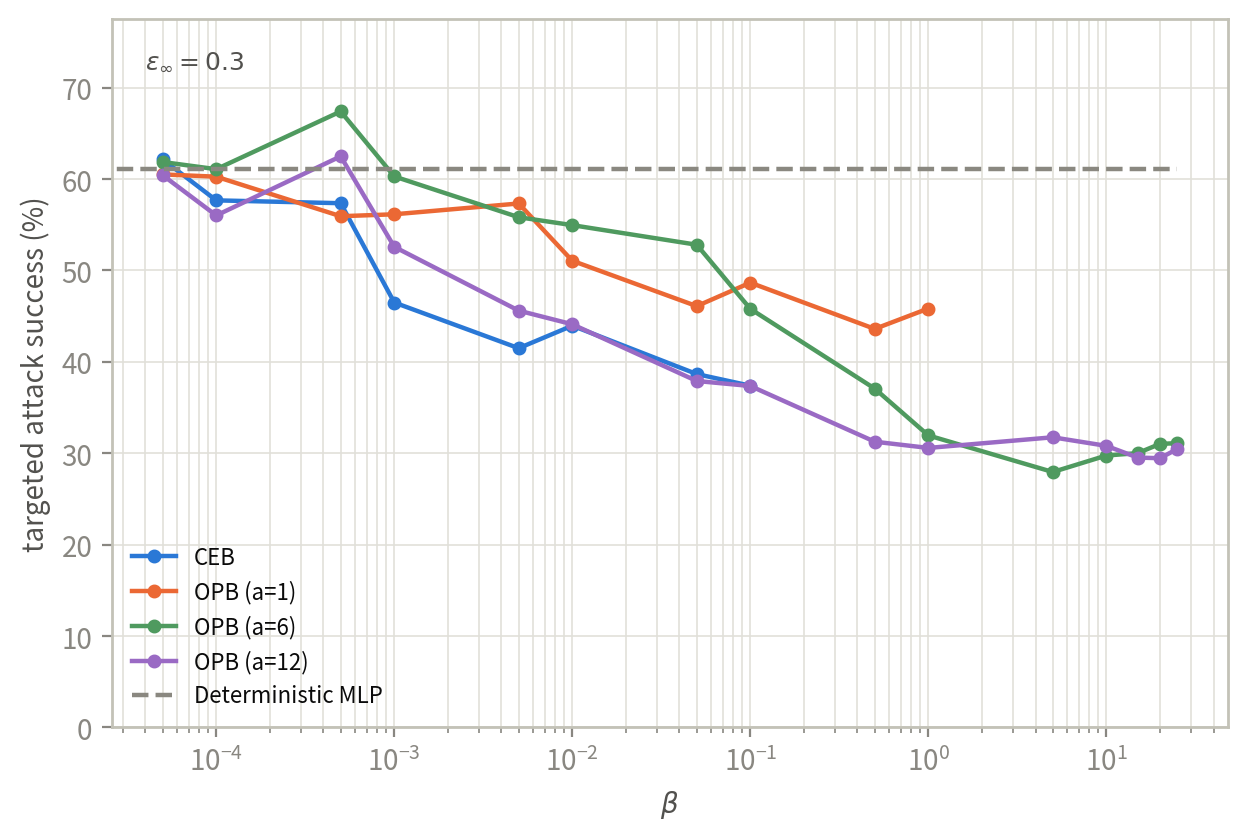
\includegraphics[width=0.48\linewidth]{figures/fig_adv_targeted_linf_mnist.png}\hfill
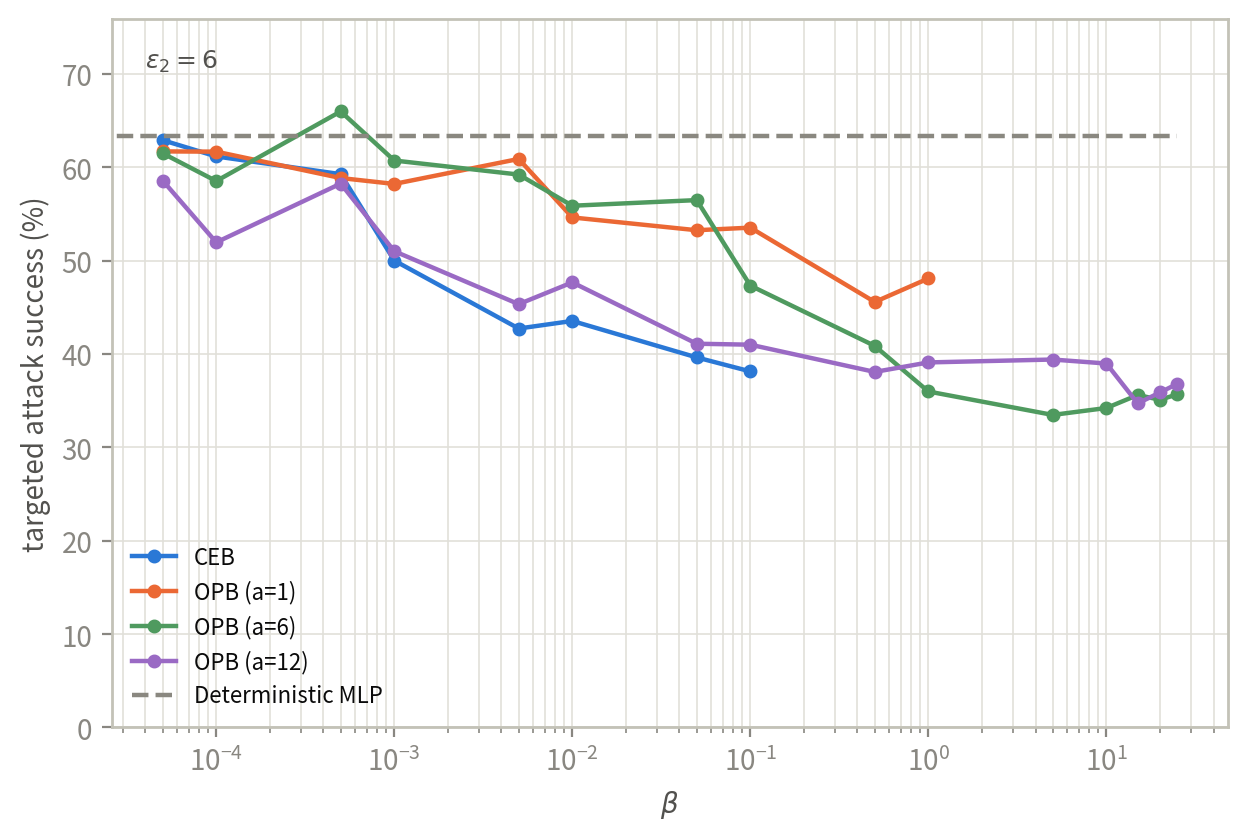
\includegraphics[width=0.48\linewidth]{figures/fig_adv_targeted_l2_mnist.png}
\caption{Targeted PGD attack success rate against $\beta$ (log scale) on MNIST
(MLP backbone): target class $0$, $20$ steps, EOT-10 gradients and 10-sample
MC predictions on the stochastic path. (a) $L_\infty$, $\varepsilon = 0.3$;
(b) $L_2$, $\varepsilon = 6.0$. The dashed grey line is the deterministic MLP
baseline. Every curve is drawn only over $\beta$ values with clean accuracy
above the shared $90\%$ failure threshold (CEB: $\beta \le 0.1$; OPB $a = 1$:
$\beta \le 1$; $a = 6$, $12$: full grid). Every curve falls with $\beta$, and
OPB keeps gaining robustness across its valid range: at $\beta = 25$,
OPB ($a = 6$, $12$) reach $31.1\%$/$30.5\%$ --- about $30$ points below the
baseline.}
\label{fig:adv-targeted}
\end{figure*}

Figure~\ref{fig:adv-targeted} shows the targeted-attack picture. Every curve
falls as $\beta$ grows, reproducing the CEB paper's compression--robustness
gradient under a protocol the deterministic path cannot game. Within CEB's operating range the two geometries are comparable at matched
$\beta$ (at $\beta = 0.1$ under $L_\infty$: $37.4\%$ for both CEB and OPB,
$a = 12$), but the $\beta$ axis again hides the compression gap --- at
$\beta = 0.1$ CEB is the \emph{more} compressed of the two (realized
$\E[\KL] = 0.68$ vs.\ $1.23$ for OPB, $a = 12$). At compression-matched points
the two geometries are at par within run-to-run variation: OPB ($a = 12$,
$\beta = 1$; $\E[\KL] = 0.55$) attains $30.6\%$ vs.\ CEB's $37.4\%$ under
$L_\infty$, a gap inside the seed spread. The decisive margin is the
operating range. Under the shared $90\%$ failure threshold, CEB's curve ends
at $\beta = 0.1$ and OPB ($a = 1$)'s at $\beta = 1$, while the larger anchors
keep accuracy at $\approx 0.98$ out to $\beta = 25$, where their targeted
success has fallen to $31.1\%$/$30.5\%$ ($a = 6/12$) under $L_\infty$ and
$35.7\%$/$36.8\%$ under $L_2$ --- about $30$ points below the deterministic
baseline and below anything CEB attains with its accuracy intact. The
$a = 1$ truncation is itself informative: at $\beta \ge 5$ the small anchor's
posterior retains substantial stochastic variance while its means pin to the
radius-$1$ anchors, so the stochastic
path the robustness protocol evaluates on drowns in noise --- the failure mode
the larger anchors avoid. We do not over-claim: this is one
dataset and one target class.

\paragraph{Transfer attacks (gradient-masking check).}
A white-box attack could fail simply because the target model's gradients are
degenerate, crediting dead models with robustness. We follow the CEB paper's
transfer protocol as the check: generate targeted PGD adversaries on one model
(the same $20$-step, EOT-10 recipe) and evaluate them on another (10-sample MC
predictions), sweeping $\varepsilon$ over $0.05$--$0.3$ ($L_\infty$) and
$1$--$6$ ($L_2$). The models are CEB ($\beta = 0.1$, the last point of its
operating range), OPB at maximum compression ($\beta = 25$, $a = 6$; realized
$\E[\KL] = 0.40$), and the deterministic MLP baseline, whose white-box curve
reaching $61\%$ at $\varepsilon_\infty = 0.3$ confirms that the attack itself
is not broken.

\begin{figure*}[t]
\centering
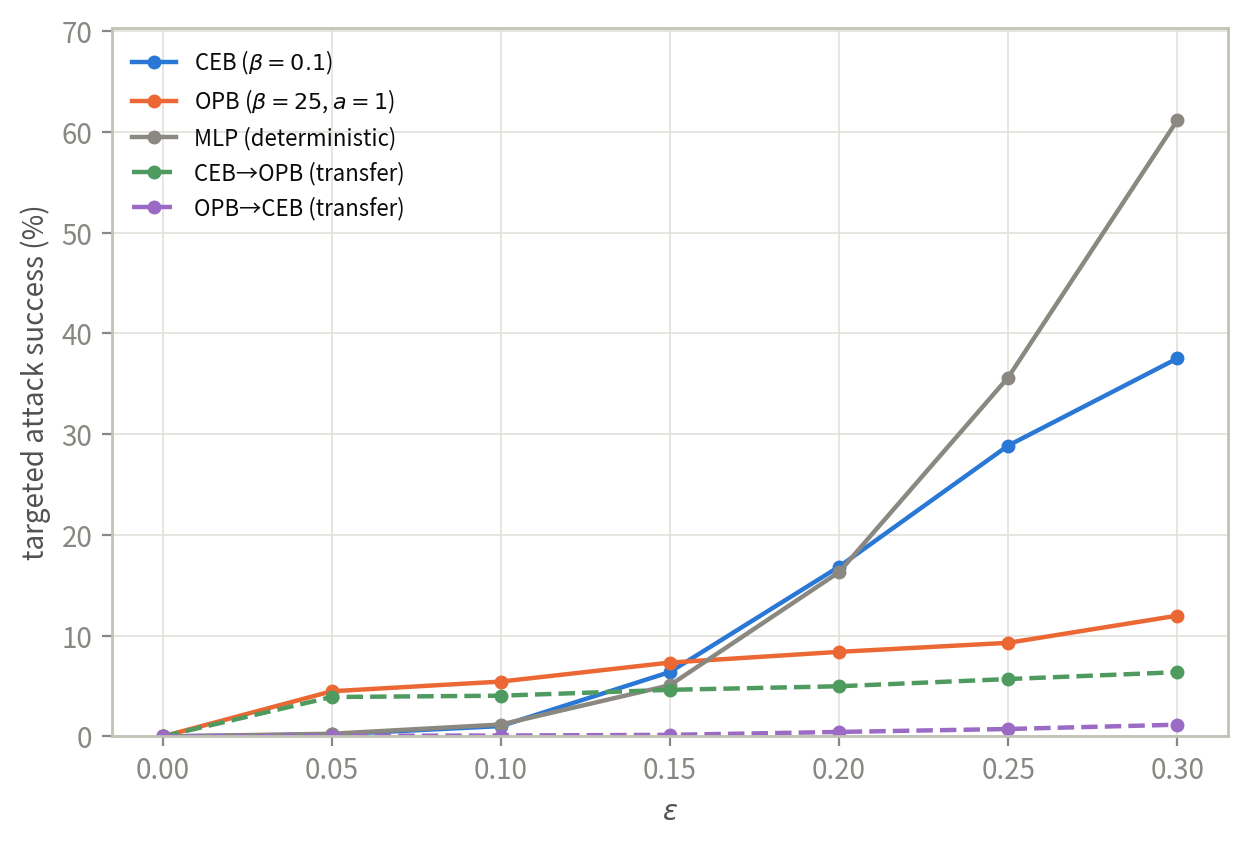
\includegraphics[width=0.48\linewidth]{figures/fig_adv_transfer_linf_mnist.png}\hfill
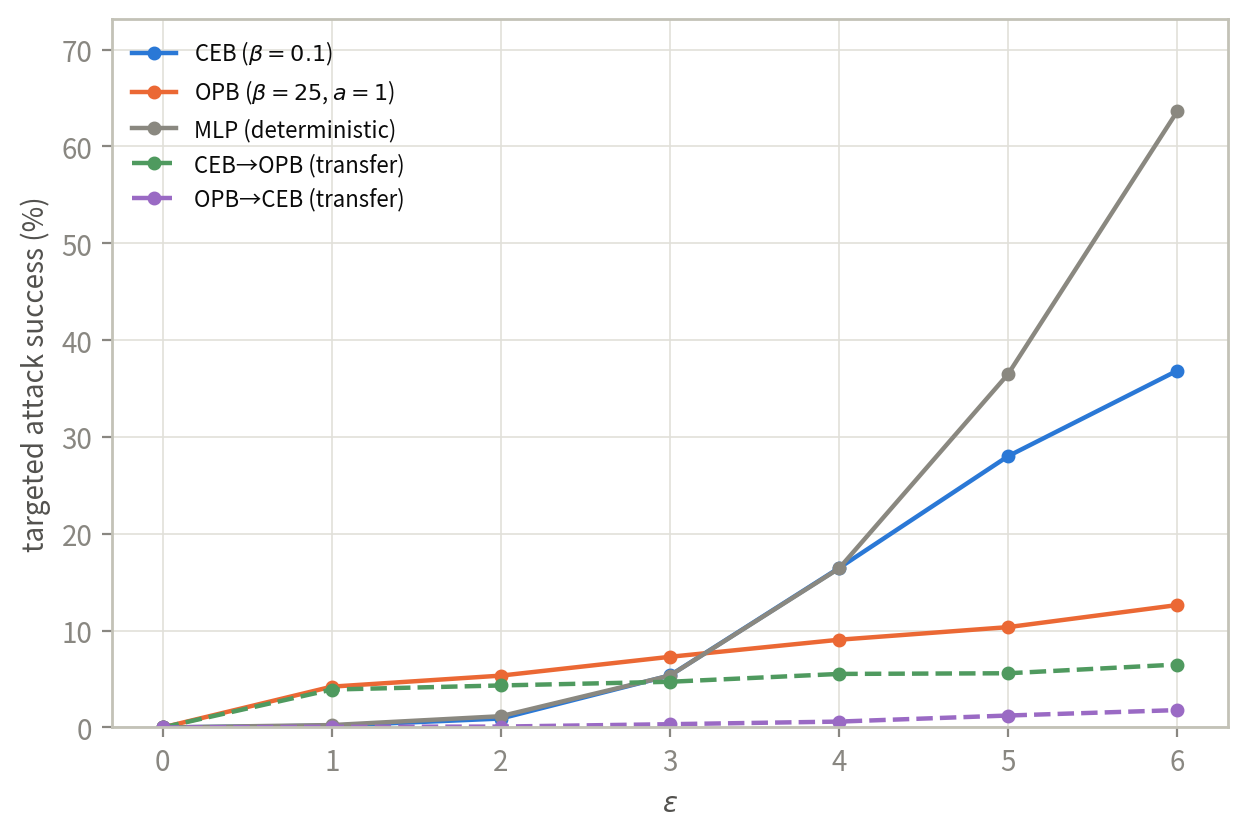
\includegraphics[width=0.48\linewidth]{figures/fig_adv_transfer_l2_mnist.png}
\caption{Transfer attacks (gradient-masking check) on MNIST (MLP backbone):
targeted PGD adversaries generated on one model and evaluated on another,
against $\varepsilon$. (a) $L_\infty$; (b) $L_2$. Solid: white-box
self-attacks of CEB ($\beta = 0.1$), OPB ($\beta = 25$, $a = 6$) and the
deterministic MLP baseline. Dashed: transfer attacks. CEB→OPB stays an order
of magnitude below OPB's own white-box attack, so OPB's extreme-compression
robustness is not gradient masking; OPB→CEB transfers little as well ---
adversarial directions found on the strongly compressed posterior are largely
model-specific.}
\label{fig:adv-transfer}
\end{figure*}

Figure~\ref{fig:adv-transfer} reads each transfer curve against its target's
own white-box attack, not against the source. CEB→OPB tops out at $2.0\%$
($L_\infty$) and $3.4\%$ ($L_2$) --- an order of magnitude below OPB's own
white-box attack ($30.2\%$/$35.4\%$) --- so the extreme-compression robustness
of OPB survives adversaries that never touch its gradients: it is geometry,
not gradient masking. The reverse direction transfers little as well
($\le 3.8\%$/$5.9\%$, against CEB's own white-box $38.2\%$/$37.9\%$):
adversarial directions found on the strongly compressed posterior are largely
model-specific, so neither model's robustness is an artifact of the other's
gradients.

% =====================================================================
\subsection{Mechanism analysis: posterior geometry and tied prediction}
\label{sec:mechanism}
% =====================================================================

The main sweep compares predictive performance. This section separately evaluates
the proposed mechanism on two representative settings, MNIST (MLP, classification)
and California Housing (MLP, regression), trained at the matched compression
$\beta = 0.1$ with anchor scale $a = \rho = 12$. The table is a
matched-configuration geometric snapshot; Section~\ref{sec:direct-mismatch} then
measures the theoretical mismatch directly across compression strengths.

\paragraph{The prior.} CEB's reference is arbitrary and drifts across seeds: the
mean off-diagonal cosine of its learned class-prior table is
$0.119 \pm 0.002$, and the scale of its learned regression axis varies by
$2.07 \pm 0.88$ across runs. The constructed prior has no such freedom: the OPB
class priors are exactly orthogonal (off-diagonal cosine $0$, pairwise distance
$\sqrt{2}\,a = 16.97$), and the EPB axis is fixed at $\rho = 12.000$ with exact
isometry through the origin, both verified at machine precision.

\input{result3}

\paragraph{The posterior.} Table~\ref{tab:mechanism} shows that this geometry
transfers to the posterior. On classification the posterior class centers are
nearly orthogonal (the mean off-diagonal Gram cosine is $5.9\times$ lower than
CEB's) and sit at radius $\lVert\bar c\rVert = 11.00$ ($92\%$ of $a$), with
$2.5\times$ lower cross-seed drift; the Fisher ratio is comparable
($15.3$ vs.\ $15.7$, reported as is). On regression the posterior lives
essentially \emph{on} the isometric axis: the off-axis residual fraction is
$141\times$ lower than CEB's, and the axial slope tracks $\rho$ with $3.8\times$
lower cross-seed variation. The slope is $9.22$ rather than $\rho = 12$ because
the encoder's uncertainty shrinks the posterior along the axis (the slope
equals $\rho \cdot R^2_{\mathrm{axis}}$, as $12 \times 0.78 \approx 9.4$), and the
axis \emph{direction} itself can rotate rigidly with the representation (mean
direction cosine $0.03$--$0.06$ for both models), so the discriminative
stability evidence is the scale, not the direction.
Figures~\ref{fig:mechanism-gram} and~\ref{fig:mechanism-axis} show both
mechanisms directly.

\begin{figure*}[t]
\centering
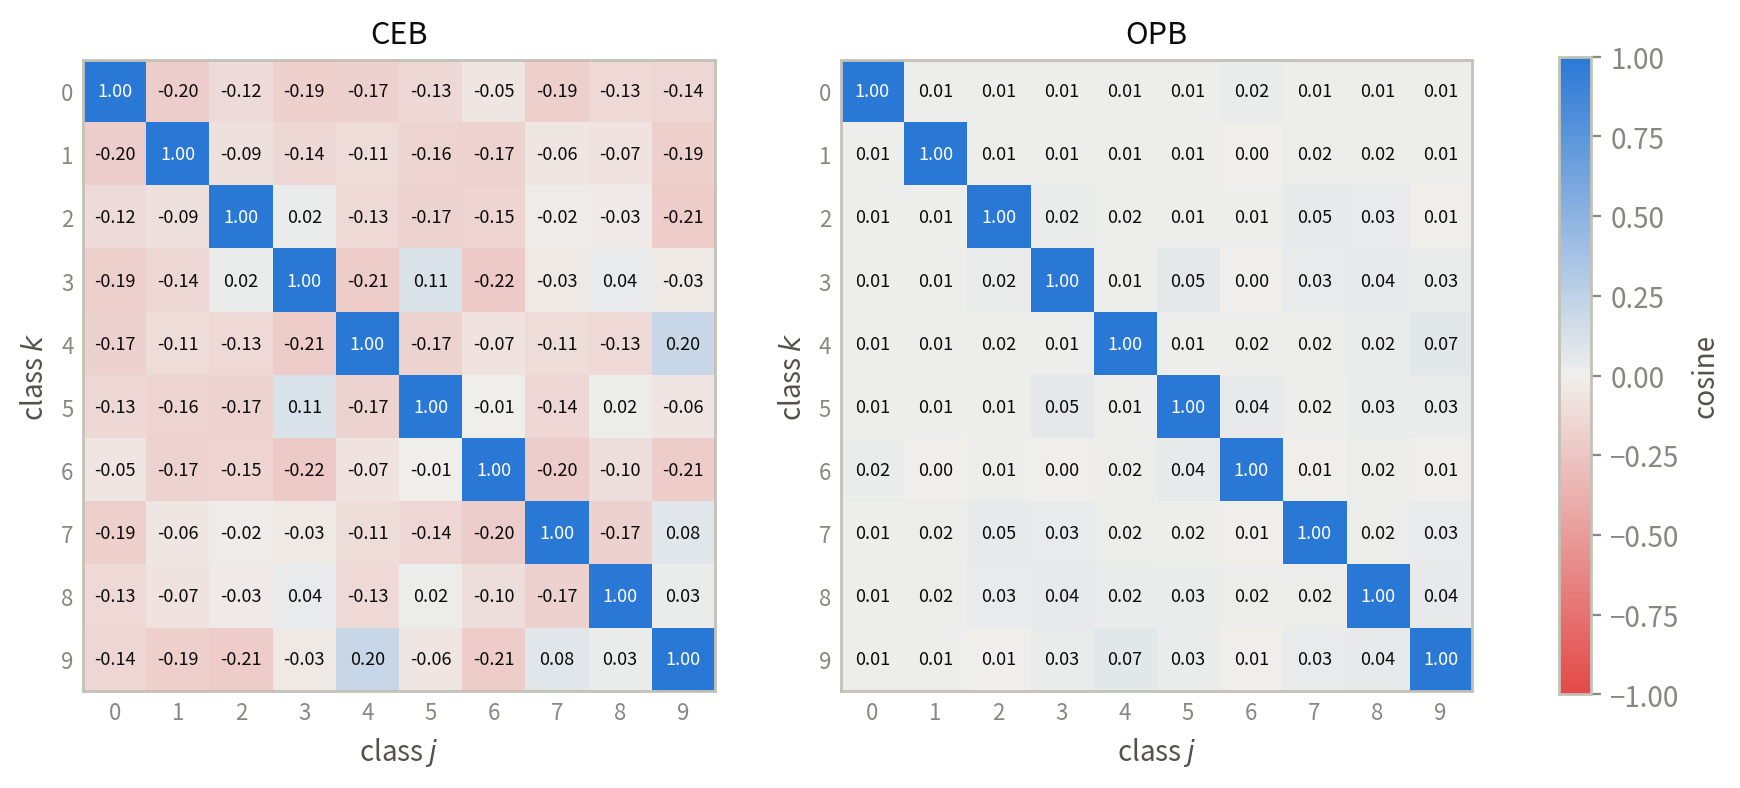
\includegraphics[width=\linewidth]{figures/fig_mechanism_gram.png}
\caption{Pairwise-cosine Gram matrix of the posterior class centers on MNIST,
averaged over five runs. OPB is nearly diagonal: the posterior centers are
orthogonal; CEB shows no such structure.}
\label{fig:mechanism-gram}
\end{figure*}

\begin{figure*}[t]
\centering
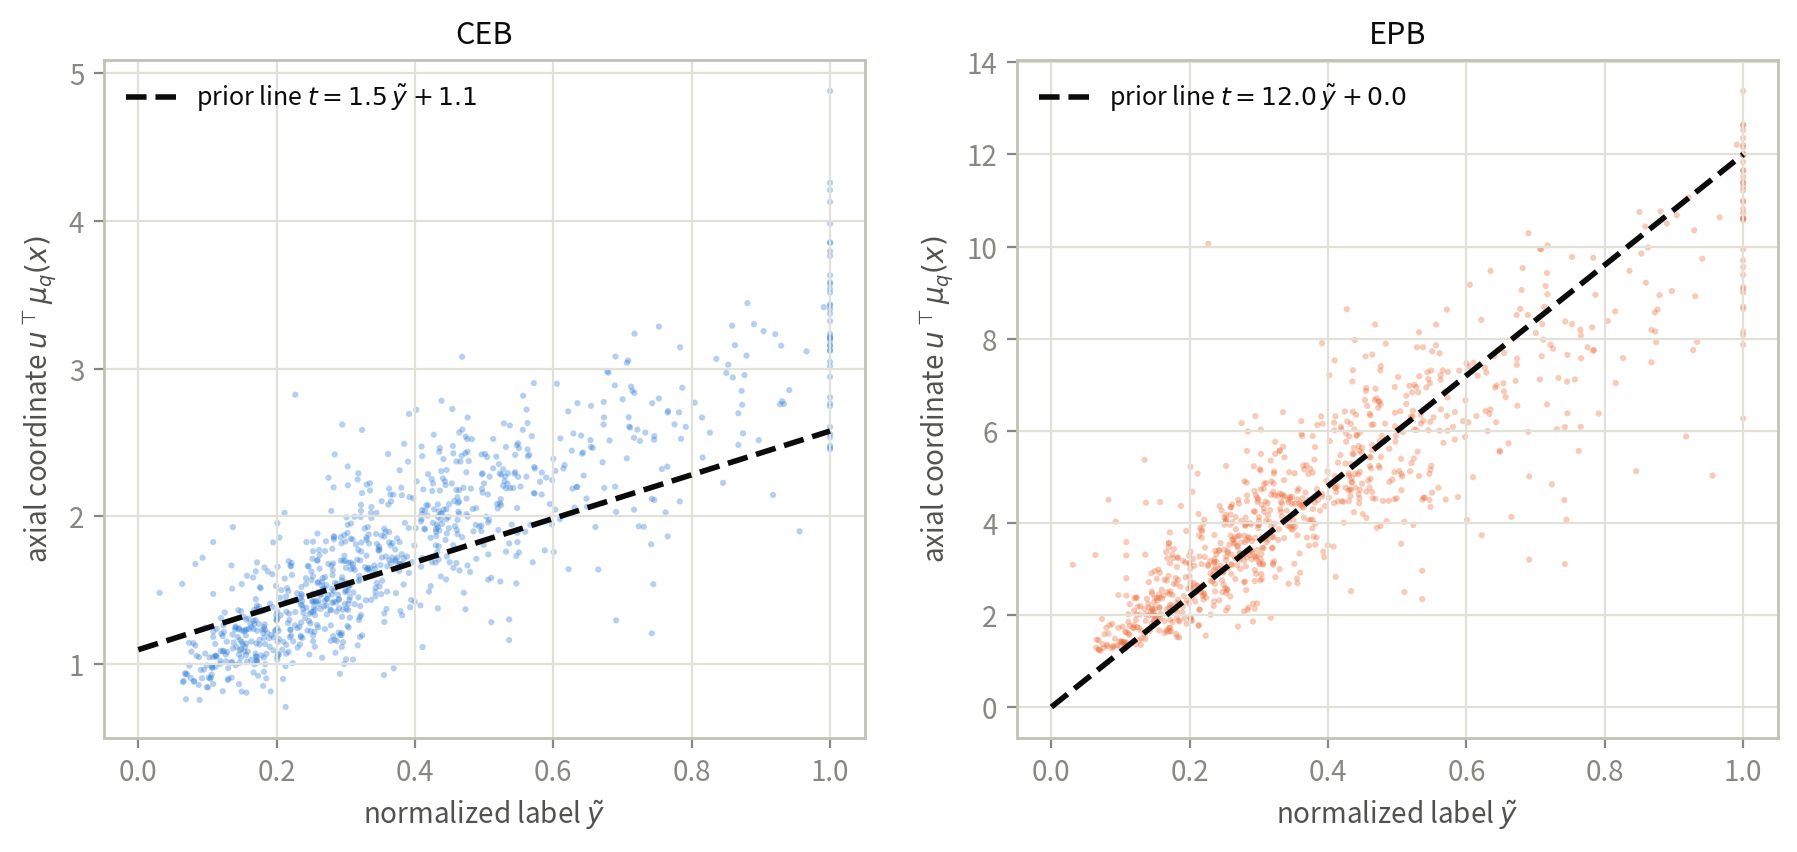
\includegraphics[width=\linewidth]{figures/fig_mechanism_axis.png}
\caption{The axial coordinate $u^{\top}\mu_q(x)$ against the normalized label on
Housing (one representative run per model). The EPB posterior hugs the prior line
$\rho\tilde y$, shrunk toward $\rho\,\mathbb{E}[\tilde y \mid x]$ by the
encoder's uncertainty.}
\label{fig:mechanism-axis}
\end{figure*}

\paragraph{Prediction reads off the geometry.} Both heads of
Section~\ref{sec:variants} have no free parameters. At the matched configuration
the anchor-energy classifier attains $98.44\%$ test accuracy against CEB's
$98.16\%$ on MNIST, and the tied projection head attains $R^2 = 0.778$ against
CEB's $0.491$ on Housing: under this strong compression CEB collapses while the
geometric readout retains the signal, consistent with the main-table GPB column
(Section~\ref{sec:main-results}) and with the nearest-anchor analysis of the
appendix. At this matched configuration, the evidence supports both links of the
mechanism: the constructed prior is accompanied by the declared posterior geometry,
and a zero-parameter rule that reads that geometry carries the prediction. This is
mechanism evidence rather than a verification of the comparator inequality.

\subsubsection{Direct mismatch analysis across compression strengths}
\label{sec:direct-mismatch}

The preceding snapshot uses geometric proxies at one operating point. We now measure
the mismatch in Proposition~\ref{prop:pgib-separation} directly over the complete
compression grids of ImageNet-100 (MLP) and Cal.\ Housing (MLP), with five seeds per
point and no missing checkpoints. For each checkpoint, we set
$\widehat\tau^2_{\max}$ to the largest conditional-reference variance realized over
the class table (classification) or test labels (regression), and compute
\begin{equation}
\widehat D=\frac{1}{N}\sum_{n=1}^{N}
\frac{\|\mu_\phi(x_n)-m_\theta(y_n)\|^2}{2\widehat\tau^2_{\max}}.
\label{eq:empirical-direct-mismatch}
\end{equation}
This is a finite-test diagnostic using a checkpoint-wise empirical variance bound, not
an estimate of a population-wide constant. KL uses each sample's actual diagonal prior
variance and is reported separately. CEB is included only as a descriptive mismatch
reference; because its class means have no declared separation, no GPB separation bound
is applied to it. Full definitions and pair-level diagnostics are in
Appendix~\ref{app:direct-mismatch}.

\paragraph{Classification.} On ImageNet-100, OPB's mismatch decreases monotonically
with compression at fixed scale: for $a=6$, $\widehat D$ falls from $62.3$ at
$\beta=5\cdot10^{-5}$ to $2.54$ at $\beta=25$. For each class pair $(i,j)$ we compare
the posterior-center distance $S_{ij}=\|m_i-m_j\|$ with the raw empirical lower bound
\begin{equation}
\widehat{\mathrm{LB}}_{ij}=\sqrt{2}a
-\sqrt{2\widehat\tau^2_{\max}\widehat D_i}
-\sqrt{2\widehat\tau^2_{\max}\widehat D_j}.
\label{eq:empirical-class-separation-bound}
\end{equation}
At $\beta=25$, this bound is positive for $96.9\%$ of class pairs at $a=12$
(mean lower bound $3.95$), $62.3\%$ at $a=6$, and none at $a=1$. The last case is
informative rather than contradictory: with $a=1$ the posterior centers collapse at
$\beta=25$ (mean $S_{ij}=0$), so the small declared margin is entirely consumed by
mismatch. At the other end, $a=6$ overshoots the frame at
$\beta=5\cdot10^{-5}$ ($S/(\sqrt2a)=1.39$); this ratio falls to $0.51$ at
$\beta=25$ as compression pulls the posterior inward. Every applicable
seed--checkpoint pair has non-negative separation slack to numerical tolerance, and
the Jensen check on every class also holds. These are consistency checks of an
unconditional inequality, not independent evidence for an optimization rate.

\paragraph{Regression.} On Housing with $\rho=6$, $\widehat D$ falls from $0.264$
at $\beta=5\cdot10^{-5}$ to $0.026$ at $\beta=25$, while $R^2$ changes only from
$0.786$ to $0.767$. This separates the mechanism measurement from the performance
comparison: a tenfold mismatch reduction need not imply a comparable task-metric gain.
The mismatch is almost entirely axial (a representative axial contribution is about
$0.2$, against an off-axis contribution of about $0.004$), and the normalized axial
slope remains $0.73$--$0.77$: the posterior follows the declared axis but at roughly
three quarters of its scale. With finite label bins and the quantization correction of
Remark~\ref{rem:pgib-binning}, $43\%$ of bin pairs retain a positive lower bound. The
mean bound is negative and the actual bin-center distances lie about $25\%$ below the
prior isometry, so the bound is consistent but conservative. Small-$\beta$, large-$\rho$
variance-explosion checkpoints are retained; their enlarged
$\widehat\tau^2_{\max}$ can reduce the normalized $\widehat D$ even while the KL
variance term grows, which is why the components in Fig.~\ref{fig:direct-mismatch}
must be read together.

\begin{figure*}[t]
\centering
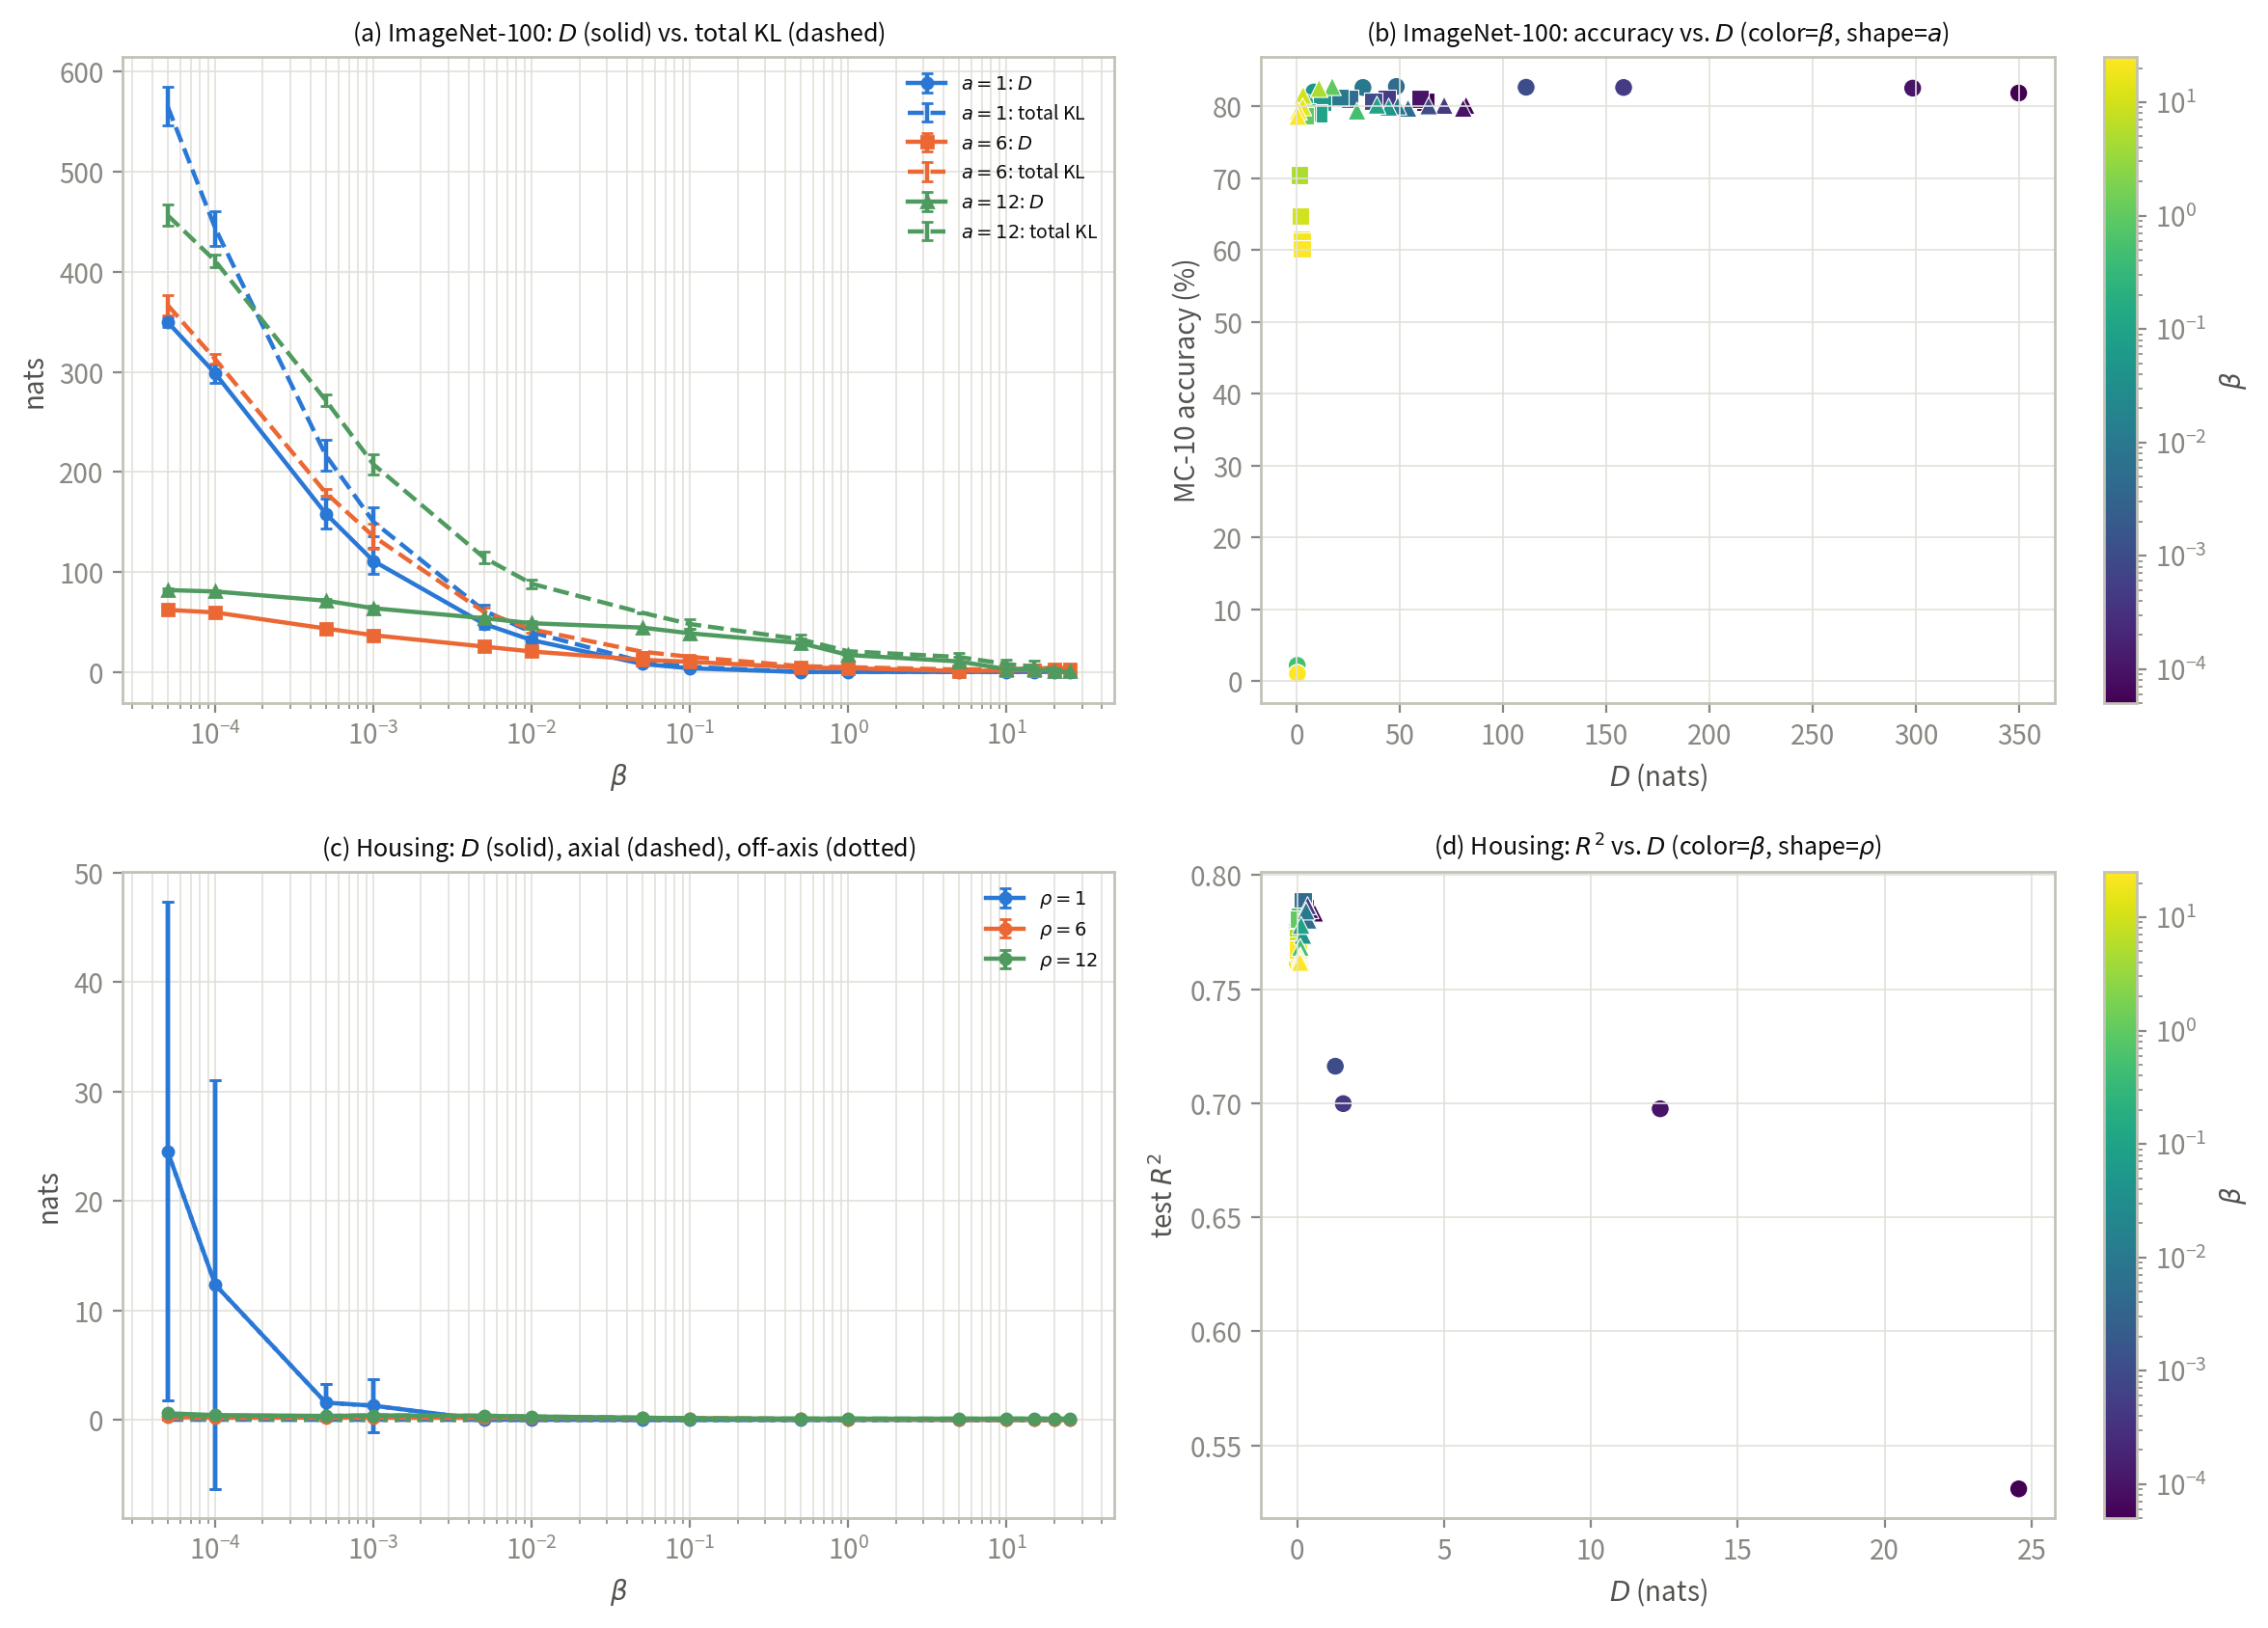
\includegraphics[width=\linewidth]{figures/fig_mismatch_main.png}
\caption{Direct mismatch diagnostics over the full compression sweeps. (a)
ImageNet-100 anchor mismatch $\widehat D$ and total KL against $\beta$, by anchor
scale. (b) MC-10 accuracy against $\widehat D$; color denotes $\beta$ and marker shape
the anchor scale. (c) Cal.\ Housing mismatch against $\beta$, decomposed into axial and
off-axis contributions. (d) Test $R^2$ against $\widehat D$. Means and standard
deviations are over five seeds; no checkpoint is omitted.}
\label{fig:direct-mismatch}
\end{figure*}

The two tasks expose complementary limits of the geometric claim. Classification has
a discrete declared margin, and sufficiently large anchors leave an informative
positive separation certificate for most class pairs. Regression transfers direction
more clearly than scale, and its finite-bin lower bound is often vacuous. Neither
observation turns benchmark accuracy into a test of Theorem~\ref{prop:pgib-alignment};
they directly evaluate the realized mismatch on which the unconditional
Proposition~\ref{prop:pgib-separation} depends.

% =====================================================================
% =====================================================================
% Related work
% =====================================================================
\section{Related work}
\label{sec:related}

\paragraph{Information bottleneck and conditional compression.}
The information bottleneck (IB) principle formulates representation learning as
retaining information about a target while discarding information about the input
\citep{tishby2000information}. Deep VIB turns this principle into a neural
objective by using a reparameterized stochastic encoder and a variational marginal
prior \citep{alemi2017deep}. Nonlinear and non-parametric bottleneck variants study
alternative variational bounds and distance-based estimates of the information in a
representation \citep{kolchinsky2017nonlinear}. The deterministic-scenario analysis
of \citet{kolchinsky2019caveats} further shows that the usual IB multiplier can fail
to sweep an interior information--accuracy trade-off when labels are deterministic,
motivating the squared-IB functional, which squares the compression term and
restores the interior trade-off.

The conditional entropy bottleneck (CEB) replaces the marginal reference of VIB by a
label-conditional reference and thereby targets conditional residual information
\citep{fischer2020conditional}. Comparisons of variational bounds clarify when this
conditional reference is tighter than a marginal one
\citep{geiger2020variational}. CEB has also been applied to large-scale visual
representations and robustness evaluations \citep{fischer2020robustness,lee2021compressive},
while multivariate extensions retain the same variational bottleneck viewpoint
\citep{abdelaleem2025deep}. These methods leave the relationships among distinct
conditional reference means unspecified. GPB keeps the CEB posterior and its single
conditional KL, but restricts the reference family itself: OPB declares a class
frame and EPB declares a label-distance-preserving axis.

\paragraph{Information bottleneck for robust representations.}
Several works use a bottleneck to suppress nuisance or non-robust information. The
HSIC bottleneck adds layer-wise dependence penalties and analyzes adversarial
robustness \citep{wang2021hsic}. Adversarial Information Bottleneck explicitly
incorporates adversarial objectives \citep{zhai2022adversarial}, and an NLP-specific
variant separates task-relevant robust features from manipulable features
\citep{zhang2022nl_ib}. Causal Information Bottleneck uses a causal decomposition
for the same robust-feature goal \citep{hua2022causal}. These approaches modify the
information criterion, feature selection, or training examples. In contrast, the
geometric constraint in GPB is placed on the conditional prior and is evaluated with
the ordinary CEB KL, so adversarial robustness is improved by the declared geometry
itself, without any additional objective.

\paragraph{Geometric classification representations.}
Neural-collapse studies document an approximately simplex-ETF arrangement of class
means and classifier directions near the terminal phase of training
\citep{papyan2020prevalence,zhu2021geometric_nc}. Other works impose related
geometry directly: orthogonal classifier weights can improve adversarial
robustness \citep{xu2022orthogonal}; ETF classifiers have been used for early exit
\citep{ji2023etf}; and fixed or hierarchy-aware frames have been used to reduce
classifier bias or mistake severity \citep{tong2023fixed_frame}. Prototype-based
constructions date back to equidistant prototype embeddings
\citep{deng2014equidistant}; Neural Collapse by Design trains features and
prototypes jointly on the unit hypersphere so that the global optimum of the NONL
contrastive objective is exactly the simplex ETF \citep{koromilas2026neural},
which we include as a classification-only comparison baseline. The connection
between neural collapse, supervised contrastive learning, and an information
bottleneck has also been analyzed explicitly \citep{wang2023ib_nc}.

These works constrain features, classifier weights, or prototypes through a
classification loss or a fixed readout. OPB addresses a different object: the
label-conditional Gaussian prior in the bottleneck. Its polar/QR frame is recomputed
from the prior encoder, and the anchor-energy classifier reads the same frame without
introducing an independent classifier scale. Thus the geometric class code and the
conditional KL are coupled during training.

\paragraph{Distance-preserving regression and geometric priors.}
Isometric representation learning has traditionally focused on preserving distances
on a data manifold, including deep extensions of isomap-style mappings
\citep{pai2022isometric}, and orthogonal label regression has been used as a
discriminative device in domain adaptation \citep{luo2023doll}; these methods
constrain a deterministic feature map. The regression information-bottleneck
literature, including divergence-based bounds, provides complementary compression
objectives rather than a geometric prior construction \citep{yu2024csd_ib}, and
AdaCap pairs a permutation-based contrastive loss with a Tikhonov closed-form
output layer for small-sample tabular regression \citep{belucci2026adacap}, which
we include as a regression-only comparison baseline. In contrast, EPB declares the
label metric in the mean map of a conditional Gaussian prior: after
standardization the prior means lie on a scaled axis, so latent prior distances
equal the declared label distances, the same axis being the tied regression
readout and the target of the conditional KL. EPB is thus a conditional-prior use
of distance geometry, not a new distance-preserving primitive.

\paragraph{Geometry-aware information bottlenecks.}
Recent work has used the phrase geometric information bottleneck in several distinct
settings. A variational recommender learns a geometric prior for explanation
generation \citep{yan2024geometric_ib}; a data-scarcity formulation penalizes latent
curvature and intrinsic dimension \citep{katende2025vgib}; and activation steering
uses orthogonal subspaces to control language-model interventions
\citep{doan2026geometric_ib}. A concurrent analysis studies the relationship between
information compression and class-wise geometric compression in CEB networks
\citep{adilova2026geometric_compression}. These studies make geometry an important
representation concern, but they do not use the same conditional Gaussian prior for
both compression and prediction, nor do they provide the OPB/EPB alignment-to-
separation construction considered here.

Table~\ref{tab:geometry-boundary} summarizes this object-level distinction: the
geometric primitive is shared with several preceding lines of work, but its role in
the objective is different, as OPB anchors are constrained class centers serving
simultaneously as Gaussian-prior means, KL targets, and readout anchors. OPB is not
an ETF construction: its anchor Gram matrix is $a^2 I_K$ (zero pairwise inner
products), whereas a centered simplex ETF has constant negative off-diagonal inner
products in a $(K-1)$-dimensional subspace.

\begin{table*}[t]
\centering
\footnotesize
\setlength{\tabcolsep}{2pt}
\renewcommand{\arraystretch}{1.12}
\caption{Object-level distinction between the related methods and GPB. IB KL:
the method's constraint enters an information-bottleneck KL term; Tied readout:
the readout is tied to the constrained geometry; Fixed / hierarchy: fixed or
hierarchy-aware frames; Isometric maps: isometric feature maps.}
\label{tab:geometry-boundary}
\begin{tabular}{>{\centering\arraybackslash}m{2.2cm} >{\centering\arraybackslash}m{2.4cm} >{\centering\arraybackslash}m{1.0cm} >{\centering\arraybackslash}m{1.6cm} >{\centering\arraybackslash}m{2.8cm} p{2.9cm}}
\hline
Approach & Declared geometry & IB KL & Tied readout & Stochastic posterior & Constrained object \\
\hline
Prototype methods & $\times$ & $\times$ & $\times$ (partial) & $\times$ (mostly) & prototypes or features \\
ETF / orthogonal & \checkmark & $\times$ & \checkmark & $\times$ (mostly) & classifier weights or feature directions \\
Fixed / hierarchy & \checkmark & $\times$ & varies & $\times$ (mostly) & feature coordinates or a frame \\
Isometric maps & \checkmark & $\times$ & varies & $\times$ (mostly) & feature map \\
CEB & $\times$ & \checkmark & $\times$ & \checkmark & label-conditional reference \\
GPB (OPB / EPB) & \checkmark & \checkmark & \checkmark & \checkmark & label-conditional Gaussian prior means \\
\hline
\end{tabular}
\end{table*}


% =====================================================================
\section*{AI use statement}
% =====================================================================

(This section is \textbf{required} and does not count toward the page limit.)

In this work, we used generative AI tools for drafting and editing portions of
the code and of this manuscript. All AI-assisted content was manually reviewed
and verified by the authors; experimental results and theoretical claims were
produced and checked by our own code and analysis. We take responsibility for
the final content of this work, including text, claims or artifacts produced
with the aid of generative AI.

\section*{Reproducibility statement}

The code, hyperparameter grids, and evaluation protocol are described in
Section~\ref{sec:setup}; the geometric prior is stateless (no EMA or prototypes)
and the orthogonalization is exact wherever defined (Assumption~\ref{ass:fullrank}).
All datasets are public, with preprocessing steps given in the release. Proofs
of all statements are collected in the appendix. Statistical claims use the
paired bootstrap confidence intervals and non-inferiority margin described in
Appendix~\ref{app:main-ci}.

\section*{Acknowledgments}

% 待填：经费与致谢信息（模板要求放在文末）

\bibliography{paper_refs}
\bibliographystyle{iclr2027_conference}


% =====================================================================
\appendix
\section{Deferred proofs, construction details, and scope}
\label{app:deferred}
% =====================================================================

\subsection{Failure diagnosis}
\label{app:diagnosis}

\begin{proposition}[Dead knob, following Caveat~1 of \citet{kolchinsky2019caveats}]
\label{prop:dead}
Assume $Y = f(X)$. For every $\gamma > 0$, the CEB objective
$L_\gamma(Z) := I(X;Z|Y) - \gamma I(Y;Z)$ is minimized exactly on the corner family
$\{Z : I(Y;Z) = H(Y),\; I(X;Z|Y) = 0\}$, and the map
$\gamma \mapsto \bigl(I(X;Z^*|Y),\, I(Y;Z^*)\bigr)$ is constant. Consequently no
interior point of the IB curve is ever a Lagrangian minimizer of CEB, over the entire
parameter range.
\end{proposition}

\begin{proof}[Proof sketch (see \citet{kolchinsky2019caveats} for the full argument)]
By the chain rule, $L_\gamma(Z) = I(X;Z) - (1+\gamma)I(Y;Z)$; the data-processing
inequality gives $L_\gamma \ge -\gamma H(Y)$, attained exactly at the corner
$Z = Y$. In the Caveats paper's maximizing convention this is their Eq.~7 with
$\beta' = 1/(1+\gamma) \in (0,1)$, the range in which every maximizer is pinned at the
copy corner.
\end{proof}

The corner is a single point of the information plane and an entire equivalence class
of representations; the objective is exactly indifferent within the class, and neither
the objective nor the certificate records which member the optimizer reaches. In the
deterministic scenario this corner \emph{is} the MNI point, so CEB's declared target
and the degenerate attractor coincide. The Caveats paper repairs this by squaring the
compression term; our anchored reference supplies the same strict convexity by a
different mechanism, without squaring: a quadratic displacement term built into the
KL by construction (Proposition~\ref{prop:opb-sweep} below). We present this as a
mechanism connection to the Caveats fix, not as a new solution of the deterministic
degeneration.

\begin{proposition}[Retention blindness on $T_\alpha$]
\label{prop:flat}
On the manifold $T_\alpha = B_\alpha \cdot Y$ of \citet{kolchinsky2019caveats}
(their Eq.~6), a family that depends on $Y$ alone, $I(X;T_\alpha|Y) = 0$ for
every $\alpha$, and with the optimal backward encoder and classifier,
$I(X;T_\alpha|Y) = 0$ and
$\CE(T_\alpha) = H(Y) - I(Y;T_\alpha) =: \delta_\alpha$: the certificate reads $0$
from the total collapse ($\alpha = 0$) to the full copy ($\alpha = 1$), while the
retained label information $I(Y;T_\alpha)$ sweeps the whole axis. Tightness of the
certificate is therefore compatible with retaining all, part, or none of $Y$: the
certificate records nothing about how much label information the code retains.
\end{proposition}

\begin{proof}
$T_\alpha$ is a function of $Y$ alone, hence $T_\alpha \perp X \mid Y$ and
$I(X;T_\alpha|Y) = 0$. By the decomposition behind Eq.~\eqref{eq:gap},
$\E\KL(q_\phi(z|X)\|r(z|Y))=I(X;Z|Y)+\E_Y\KL(q_\phi(z|Y)\|r(z|Y))$, with the true
backward encoder the gap term vanishes and the certificate is tight,
$I(X;T_\alpha|Y) = 0$, and the optimal
classifier attains $\langle \log c(y|z)\rangle = -H(Y|T_\alpha)$, i.e.\
$\CE = H(Y|T_\alpha) = \delta_\alpha$.
\end{proof}

\begin{remark}[The objective on $T_\alpha$ is $\beta$-independent and strictly prefers the full copy]
\label{rem:flatness}
On $T_\alpha$ the compression term contributes nothing
($I(X;T_\alpha|Y) \equiv 0$), so
the objective reads $L = \CE + \beta\,I(X;T_\alpha|Y) = \delta_\alpha$, independent of
$\beta$ and strictly minimized at $\alpha = 1$ (the full copy). No certified residual
is produced anywhere on the manifold; the blindness is that the certificate cannot
tell the optimizer --- or the analyst --- where on the retention axis the code sits.
\end{remark}

\emph{Scope of the comparison argument.} Theorem~\ref{prop:pgib-alignment} applies to
arbitrary $P_{XY}$ and every feasible comparator in the fitted model class; it does not
require $q(z|x)=p_\theta(z|y)$. Its usefulness depends on the comparator KL. Label
ambiguity, limited encoder capacity, and covariance misspecification produce the
non-zero floor made explicit in Proposition~\ref{prop:pgib-ambiguity-decomposition}.
The stronger statement that this floor is zero still requires the assumptions of
Corollary~\ref{cor:pgib-exact-alignment}: deterministic labels, exact posterior--prior
matching, and a compatible head. We do not assume those exact-realizability premises
for the real-data benchmarks. Their performance comparison evaluates utility, while
their structural diagnostics report realized mismatch and geometry. The controlled
known-noise experiment instead evaluates the ambiguity term where its population value
is analytic, including the deterministic distribution as its zero-floor special case.

\subsection{Proofs of the comparator and separation guarantees}

\begin{proof}[Proof of Theorem~\ref{prop:pgib-alignment}]
Since the GPB prior covariance is $\Sigma_\theta(y)=\tau^2I_d$ with
$\tau^2=\tau_{\max}^2=1$, the Gaussian KL contains the mean term
$\frac12(\mu_\phi(x)-m_\theta(y))^\top\Sigma_\theta^{-1}(y)(\mu_\phi(x)-m_\theta(y))
=\|\mu_\phi(x)-m_\theta(y)\|^2/(2\tau^2_{\max})$. Hence
$\mathcal D(\widehat w)\le\mathcal K(\widehat w)$. For any feasible $w_0$ in the
same family, $\varepsilon$-optimality of $\widehat w$, $\ell\ge0$, and $\beta>0$
give
\begin{equation*}
\beta\mathcal K(\widehat w)
\le \mathcal R(\widehat w)+\beta\mathcal K(\widehat w)
\le \mathcal R(w_0)+\beta\mathcal K(w_0)+\varepsilon.
\end{equation*}
Division by $\beta$ proves Eq.~\eqref{eq:pgib-comparator-bound}.
\end{proof}

\begin{proof}[Proof of Theorem~\ref{thm:pgib-separation}]
Jensen's inequality gives
$\|m(y) - m_\theta(y)\| \le \sqrt{2\tau^2_{\max} D(y)}$
(the norm is convex, and $\E\|\mu_\phi(X)\|^2<\infty$ makes $m(y)$ well defined),
and the triangle inequality on
$m(y) - m(y') = (m(y) - m_\theta(y)) + (m_\theta(y) - m_\theta(y'))
+ (m_\theta(y') - m(y'))$ gives the two-level bound of
Eq.~\eqref{eq:pgib-separation}, the last step
by the definition of $\Delta(y,y')$. The first level is positive exactly
when $\Gamma_{yy'}<1$ and the declared-margin level exactly when
$\sqrt{2\tau^2_{\max}D(y)}+\sqrt{2\tau^2_{\max}D(y')}<\Delta(y,y')$; for OPB the
anchor pair distance is the constant $\sqrt2a$ of
Eq.~\eqref{eq:opb-prior}, so the declared bound satisfies $\Delta(y,y')=\sqrt2a$ and
the two conditions coincide. With equal mismatch $D$ the common condition
$\Gamma_{yy'}=2\sqrt{2\tau^2_{\max}D}/(\sqrt2a)<1$ reduces to
$D<a^2/(4\tau^2_{\max})$. For continuous labels the Jensen inequality holds
pointwise for $P_Y$-a.e.\ $y$ (regular conditional expectation), and intersecting
the two measure-one sets of valid $y$'s yields the $P_Y\otimes P_Y$-almost-everywhere
pair statement.
\end{proof}

\begin{remark}[Finite-sample estimation of the continuous case]
\label{rem:pgib-binning}
On finite samples the regular conditional expectations of the continuous case are
estimated by
binning the label axis into intervals $B_i$ with representative labels $\bar y_i$
and centers $m_i = \E[\mu_\phi(X) \mid Y \in B_i]$; the bin diameter adds a
quantization error bounded by
$\rho_{\max}\,\operatorname{diam}(B_i) + \rho_{\max}\,\operatorname{diam}(B_j)$ (by
the upper bound of Eq.~\eqref{eq:pgib-lipschitz}), which vanishes as the bins
shrink. The separation statement itself is pointwise and needs no binning.
\end{remark}

\begin{proof}[Proof of Corollary~\ref{cor:pgib-beta-transfer}]
Theorem~\ref{prop:pgib-alignment} gives
$\mathcal D(\widehat w_\beta)\le B_\beta$. For discrete labels, the tower property
gives $\mathcal D(\widehat w_\beta)=\sum_k\pi_kD(k)$, hence
$D(k)\le B_\beta/\pi_k\le B_\beta/\pi_{\min}$; for continuous labels, Markov's
inequality on the nonnegative random variable $D(Y)$ gives
$P_Y(D(Y)>B_\beta/\xi)\le\xi$. In both cases
Theorem~\ref{thm:pgib-separation} then gives
Eq.~\eqref{eq:pgib-beta-separation}. The rate statement follows
directly from the definition of $B_\beta$: with $\mathcal K(w_0)=0$ and
$\sup_\beta\varepsilon_\beta<\infty$, $B_\beta=O(\beta^{-1})$ so the certified
deficit is $O(\beta^{-1/2})$; with $\mathcal K(w_0)>0$,
$B_\beta\to\mathcal K(w_0)$ as $\beta\to\infty$.
\end{proof}

\begin{proof}[Proof of Proposition~\ref{prop:pgib-ambiguity-decomposition}]
For OPB let $A_Y:=a q_{0,Y}$. Conditional on $X$, orthonormality gives
$\E[A_Y\mid X]=a\sum_k\eta_k(X)q_{0,k}$ and
\begin{equation*}
\E\!\left[\|A_Y-\E[A_Y\mid X]\|^2\mid X\right]
=a^2\left(1-\|\eta(X)\|_2^2\right).
\end{equation*}
The conditional bias--variance identity then yields
\begin{equation*}
\E\|h(X)-A_Y\|^2
=a^2\E[1-\|\eta(X)\|_2^2]
+\E\left\|h(X)-a\sum_k\eta_k(X)q_{0,k}\right\|^2.
\end{equation*}
Adding the diagonal-Gaussian covariance term $V_0$ proves
Eq.~\eqref{eq:opb-ambiguity-decomposition}. For EPB set
$A_Y:=\rho\tilde Y u_0$. Then
$\E[A_Y\mid X]=\rho\nu(X)u_0$ and
$\E[\|A_Y-\E[A_Y\mid X]\|^2\mid X]
=\rho^2\operatorname{Var}(\tilde Y\mid X)$. The same identity plus $V_0$ proves
Eq.~\eqref{eq:epb-ambiguity-decomposition}.
\end{proof}

\begin{proof}[Proof of Corollary~\ref{cor:pgib-exact-alignment}]
For classification, the assumed comparator $q(z|x)=p_\theta(z|y)$ has
$\mathcal K(w_0)=0$. Its Bayes cross-entropy is
$C_{\mathrm G}=H(Y\mid Z_{\mathrm{align}})\le\ln K$; with shared covariance the
determinant factors cancel and its posterior is the anchor-energy rule. Applying
Eq.~\eqref{eq:pgib-comparator-bound} gives Eq.~\eqref{eq:pgib-alignment}. For
regression the aligned comparator again has zero KL. Under the tied head its error is
$(\tau/\rho)\eta$, $\eta\sim\mathcal N(0,1)$, so its standardized squared risk is
$\tau^2/\rho^2$; the same proposition gives
Eq.~\eqref{eq:pgib-alignment-regression}.
\end{proof}

\begin{proof}[Proof of Proposition~\ref{prop:opb-collapse}]
By Jensen's inequality the left side is at least
$\tfrac{1}{2\tau^2}\sum_k \pi_k \|c - a q_{\theta,k}\|^2
= \tfrac{1}{2\tau^2}\bigl(\|c\|^2 - 2a\,c^{\top}\!\sum_k\pi_k q_{\theta,k} + a^2\bigr)$.
Minimizing over $c$ gives $c = a\sum_k\pi_k q_{\theta,k}$; by orthonormality
$\|\sum_k\pi_k q_{\theta,k}\|^2 = \sum_k \pi_k^2$, yielding Eq.~\eqref{eq:opb-collapse}.
\end{proof}

\begin{remark}[What the framework constrains (and what it does not)]
\label{rem:counterexample}
The constraints of the geometric prior bind the reference, not the deployed
representation: for any orthonormal frame $\{q'_k\}$ and the class-constant posterior
$q(z|Y=k) = \mathcal{N}(a\,q'_k, \tau^2 I_d)$, the trainable frame can rotate
to match ($q_{\theta,k} \to q'_k$), yielding $\KL = 0$, $I(X;Z|Y) = 0$, and
$I(Y;Z) > 0$: a full-retention label code with a zero certificate. The framework
therefore constrains the geometric \emph{form} of the label code (precisely what CEB
left unspecified), and does not claim that the certificate meters retained label
information. In the GPB instance used by the real-data protocol, the remaining
freedom at certificate zero is the frame rotation only.
\end{remark}

\subsection{Construction details}
\label{app:construction}

\begin{assumption}[Full rank]
\label{ass:fullrank}
$U_\theta$ has full column rank wherever the polar factor and its backward pass are
evaluated; this is monitored rather than imposed by an extra loss.
\end{assumption}

\paragraph{Polar permutation equivariance.} For any label permutation matrix $P$,
\begin{equation}
Q_\theta(U_\theta P)
= U_\theta P \bigl( P^{\top} U_\theta^{\top} U_\theta P \bigr)^{-1/2}
= U_\theta \bigl( U_\theta^{\top} U_\theta \bigr)^{-1/2} P
= Q_\theta(U_\theta)\, P ,
\label{eq:opb-equivariance}
\end{equation}
since $P P^{\top} = I_K$ and the inverse square root conjugates under $P$. Permuting
the label numbering therefore permutes the anchors accordingly, and no class index
plays a distinguished role.

\begin{proposition}[Orthogonal class-prior geometry by construction]
\label{prop:opb-frame}
Under Eqs.~\eqref{eq:opb-qr}--\eqref{eq:opb-prior}, the class means
$a_k = a\,q_{\theta,k}$ have Gram matrix $a^2 I_K$: under
Assumption~\ref{ass:fullrank}, the prior
supplies a class-separated spherical code at every training step, whatever the
optimizer does.
\end{proposition}

\begin{proof}
The geometry in Eq.~\eqref{eq:opb-prior} follows from
$Q_\theta^{\top}Q_\theta = I_K$ after scaling by $a$; in particular
$\|a_i - a_j\|^2 = \|a_i\|^2 + \|a_j\|^2 - 2a_i^{\top}a_j = 2a^2$.
\end{proof}

\begin{proposition}[Anchor-energy classifier equivalence]
\label{prop:opb-energy}
The scores $s_k(z)=-\|z-aq_{\theta,k}\|^2/(2\tau^2)+\log\pi_k$ are Gaussian Bayes
scores up to a class-independent term. For uniform classes, the corresponding linear
weights are $(a/\tau^2)q_{\theta,k}$.
\end{proposition}

\paragraph{Initialization, monitoring, and re-initialization.} The posterior logvar
head is zero-initialized ($\sigma^2 = \tau^2 = 1$ at initialization, so training
starts at $\KL \approx \tfrac{1}{2\tau^2} a^2$); the prior encoder is
identity-initialized, so the initial raw matrix is $U_\theta = [e_1, \dots, e_K]$,
full column rank, with a stable polar-factor backward (the verified condition of
Assumption~\ref{ass:fullrank}). The full-rank condition is \emph{verified, not
imposed}: $\sigma_{\min}(U_\theta)$ is monitored along training and stays bounded
away from zero in the reported runs, and no additional regularizer is added to the
objective, which remains Eq.~\eqref{eq:pgib-objective} exactly. Near rank deficiency
the polar factor's gradient is delicate; should the monitor flag a near-deficient
step, the recommended handling is a re-initialization of the prior encoder (the
reported runs never triggered it).

\paragraph{Covariance protocol.} Equations~\eqref{eq:opb-prior} and
\eqref{eq:epb-prior} define the OPB and EPB instances used throughout the paper.
Their prior covariance is the fixed shared $\tau^2I$ with $\tau^2=1$ (matching the
zero-initialized posterior at $\sigma^2=1$ so training starts at
$\KL\approx a^2/(2\tau^2)$), with no learned prior-covariance parameters. The
posterior retains its learned diagonal covariance $\sigma^2_\phi(x)$, as specified
in Eq.~\eqref{eq:pgib-covariance}. Proposition~\ref{prop:opb-energy} therefore
applies verbatim: the anchor-energy readout is the exact Gaussian Bayes head of the
benchmark model. The direct diagnostics in Section~\ref{sec:direct-mismatch}
normalize by the declared $\tau^2$.

\paragraph{EPB axis choices.} Three variants of the direction: (A) \emph{fixed
axis}, $u = [1, 0, \dots, 0]$, with no trainable prior direction: the
theoretically cleanest ablation, at the price of prespecifying a latent coordinate;
(B) \emph{trainable normalized axis}, $u = W/\|W\|$ with $W$ trained and normalized
at every step, our main variant, which keeps the scale $\rho$ exact while allowing
the model to choose the axis; (C) \emph{unconstrained linear axis},
$\mu_p(y) = W \tilde y$: the simplest ablation, still isometric by linearity but
with a free scale that can shrink and weaken the geometry. We recommend (B), use (A)
to test whether the trainable rotation carries the benefit, and keep (C) as a
diagnostic. The main variant uses no bias: an affine offset cancels in pairwise
distances but is a free extra degree of matching, and $\tilde y$ is already centered.

\paragraph{EPB isometry notes.} The isometry is exact and global: any nonzero linear
map of a scalar label is isometric up to its norm, and the normalization fixes that
norm to $\rho$; unlike fixed random-feature anchors, whose pairwise distances grow
nonlinearly and saturate, the isometric axis preserves label distances at every scale
(with the price that anchor norms grow with $|\tilde y|$; a line and a fixed-radius
sphere intersect in at most two points, so isometry and equal norms cannot both hold).
All prior means lie on one line; for $y_i < y_j < y_k$ the distances add,
$\|\mu_p(y_i)-\mu_p(y_k)\| = \|\mu_p(y_i)-\mu_p(y_j)\| + \|\mu_p(y_j)-\mu_p(y_k)\|$:
order and magnitude of label differences are encoded exactly.

\paragraph{Multidimensional regression labels.} For $y \in \R^m$ ($m \le d$), the
same construction extends verbatim: take $W \in \R^{d \times m}$, its thin polar
factor $Q = W (W^{\top}W)^{-1/2}$, and the prior $\mu_p(y) = \rho\, Q\, \tilde y$,
which is isometric in the label metric; the scalar case is $m = 1$ with $Q = u$. The
label metric must be declared before standardization, otherwise ``isometric'' has no
unique meaning.

\subsection{Additional results}

\begin{lemma}[OPB KL decomposition]
\label{lem:opb-kl-decomposition}
For a diagonal posterior covariance and the prior of Eq.~\eqref{eq:opb-prior},
\begin{equation}
\KL\bigl(q_\phi(z|x)\,\|\,p_\theta^{\mathrm{OPB}}(z|y)\bigr)
= \frac{1}{2\tau^2}\|\mu_\phi(x) - a\,q_{\theta,y}\|^2
+ \frac12 \sum_{r=1}^{d}\Bigl[
\frac{\sigma_{\phi,r}^2(x)}{\tau^2} - 1 - \log\frac{\sigma_{\phi,r}^2(x)}{\tau^2}
\Bigr],
\label{eq:opb-kl-decomposition}
\end{equation}
a class-anchor mismatch term plus a variance mismatch term that is non-negative and
vanishes exactly at $\sigma_{\phi,r}^2(x) = \tau^2$ for all $r$. The mismatch term is
quadratic in the displacement to a reference whose scale and covariance cannot move:
this is the mechanism behind the strict convexity of
Proposition~\ref{prop:opb-sweep} below.
\end{lemma}

\begin{proof}
Apply the diagonal-Gaussian KL formula with posterior mean $\mu_\phi(x)$, prior mean
$a\,q_{\theta,y}$, posterior variances $\sigma_{\phi,r}^2(x)$, and the fixed prior
variance $\tau^2$.
\end{proof}

\begin{corollary}[Label-information lower bound in the aligned Gaussian model]
\label{cor:opb-fano}
Assume uniform classes and exact alignment
$q(z|Y=k) = \mathcal{N}(a\,q_{\theta,k}, \tau^2 I_d)$. The pairwise error probability
of the nearest-anchor classifier is
$P_{\mathrm{pair}} = \Phi\bigl(-\frac{a}{\sqrt{2}\,\tau}\bigr)$, with
$P_e \le \min\{1, (K-1)P_{\mathrm{pair}}\}$, and whenever the displayed bound
$\bar P_e \le 1 - 1/K$, Fano's inequality gives
$I(Y;Z) \ge \log K - h_2(\bar P_e) - \bar P_e \log(K-1)$. This links the anchor
scale-to-noise ratio $a/\tau$ to the retained label information, conditionally on the
aligned Gaussian model.
\end{corollary}

\begin{proof}
Two anchors have distance $\sqrt{2}a$ by Proposition~\ref{prop:opb-frame}; the
equal-covariance binary decision boundary is halfway between them, giving
$\Phi(-\sqrt{2}a/(2\tau))$. The union bound and Fano's inequality on
$[0, 1-1/K]$ conclude.
\end{proof}

\begin{proposition}[Joint strict convexity and unique optimum on a restricted aligned surrogate]
\label{prop:opb-sweep}
Consider the class-symmetric aligned family: every input of class $y$ is mapped to the
posterior $q_y = \mathcal{N}(s\,q_{\theta,y}, \sigma^2 I)$ ($s \ge 0$, $\sigma^2 > 0$;
anchor scale $a > 0$), and the classifier is the anchor-energy classifier of
Proposition~\ref{prop:opb-energy} (weights $w_j = c\,q_{\theta,j}$ with scale
$c = a/\tau^2$ fixed by construction). With the \emph{stochastic training code}
$z \sim q_y$ (as in the actual objective, Eq.~\eqref{eq:pgib-objective}), the
training cross-entropy is
\begin{equation}
g(s, \sigma^2) := \E_\eta\Bigl[
\ln\Bigl(1 + \textstyle\sum_{j \ne y} e^{-cs + c\sigma(\eta_j - \eta_y)}\Bigr)
\Bigr],
\qquad \eta \sim \mathcal{N}(0, I_K),
\label{eq:opb-ce-train}
\end{equation}
and the training Lagrangian is
\begin{equation}
L_\beta(s, \sigma^2) = g(s, \sigma^2)
+ \beta\Bigl[
\tfrac{1}{2\tau^2}(s-a)^2
+ \tfrac{d}{2}\bigl(\sigma^2/\tau^2 - 1 - \ln(\sigma^2/\tau^2)\bigr)
\Bigr].
\label{eq:opb-lag-train}
\end{equation}
Then for every $\beta > 0$, $L_\beta$ is strictly convex jointly in $(s, \sigma)$ and
has a unique joint minimizer $(s^*(\beta), \sigma^*(\beta))$, interior in $s$ since
$a > 0$: the stochastic training objective has a well-defined optimum, in contrast to
the deterministic IB Lagrangian, whose optimum is pinned at a corner for every $\beta$
(Proposition~\ref{prop:dead}). This is a \emph{restricted surrogate result}: it
analyzes two scalar variables on the class-symmetric aligned family, with the frame,
the anchor scale, and the classifier scale held fixed; the full OPB objective, with
its nonlinear posterior, trainable frame, and non-convex degrees of freedom, lies
outside this analysis, and the result neither establishes $\beta$-tunability of the
full objective nor makes any claim on the information plane.
The deterministic evaluation code ($z = \mu$) is the $\sigma \to 0$ limit, and
$g \ge \ln(1 + (K-1)e^{-cs})$ by Jensen (the log-sum-exp is convex), so the statement
strictly generalizes the deterministic surrogate analysis. We do \emph{not} claim here
that the map $\beta \mapsto s^*(\beta)$ is monotone or that the sweep is one-to-one:
the minimizer $\sigma^*$ responds to $\beta$ through the cross-derivative
$\partial^2 g/\partial s\,\partial\sigma$, and establishing the sign of
$\mathrm{d}s^*/\mathrm{d}\beta$ requires the full two-dimensional stationarity
analysis, which we leave open; the $\beta$-sweep is reported empirically in the
experiments. The fixed-scale condition holds for the main model by construction
(Proposition~\ref{prop:opb-energy}), so the statement describes the actual training
objective up to the aligned-family idealization. We do not analyze the free-classifier
variant on this surrogate: under the stochastic training code, a diverging classifier
scale does not produce a degenerate solution: at $\operatorname{KL} \to 0$ the
posterior variance is pinned at $\sigma^2 = \tau^2 > 0$, so the class-conditional
Gaussians overlap and the training cross-entropy of a free classifier diverges with
its scale rather than vanishing (for $K = 2$ it contains
$\E[\ln(1 + e^{-c(a + \tau\xi)})]$, whose integrand grows linearly in $c$ on the
event $\xi < -a/\tau$, which has positive probability). An analysis of the free
classifier would require an explicit classifier-norm constraint or regularizer and is
left to future work.
\end{proposition}

\begin{proof}
For each fixed $\eta$, the integrand of Eq.~\eqref{eq:opb-ce-train} is a log-sum-exp of
functions affine in $(s, \sigma)$ (the constant $1$ has slope zero and each exponential
has slope $(-c,\, c(\eta_j - \eta_y))$), hence jointly convex in $(s, \sigma)$, and the
expectation $g$ is jointly convex. No strictness is claimed for $g$: for $K = 2$ the
integrand depends on $(s, \sigma)$ only through the single linear combination
$-cs + c\sigma(\eta_2 - \eta_1)$, so its Hessian has rank one. Write the KL term as
$R(s, \sigma) := \tfrac{1}{2\tau^2}(s-a)^2
+ \tfrac{d}{2}\bigl(\sigma^2/\tau^2 - 1 - \ln(\sigma^2/\tau^2)\bigr)$; its Hessian in
$(s, \sigma)$ is
$\nabla^2 R = \operatorname{diag}\bigl(\tau^{-2},\; d\,(\tau^{-2} + \sigma^{-2})\bigr)$,
strictly positive definite for every $\sigma > 0$, so $\beta R$ is strictly convex in
$(s, \sigma)$. Hence $L_\beta = g + \beta R$ is the sum of a jointly convex and a
strictly convex function, and is strictly convex in $(s, \sigma)$. Since
$R \to +\infty$ as $s \to \infty$, $\sigma \to 0^+$, or $\sigma \to \infty$, the
sublevel sets of $L_\beta$ are compact, and the unique joint minimizer exists (by
strict convexity it is unique). For $a > 0$ the minimizer is interior in $s$: at
$s = 0$, $\partial L_\beta/\partial s = -c\,\E[p_{\mathrm{w}}] - \beta a/\tau^2 < 0$,
where $p_{\mathrm{w}}$ is the error probability of the sampled code, so $s^* > 0$.
\end{proof}

\begin{remark}[The sweep is a KL--CE surrogate curve; scope and limitations]
\label{rem:opb-scope}
Proposition~\ref{prop:opb-sweep} proves joint strict convexity and uniqueness of the
optimum for the stochastic training objective in the KL--CE plane on the aligned family
at fixed classifier scale: a restricted surrogate result, which does not establish
$\beta$-tunability of the full OPB objective, and in any case not a statement on the
information plane of the Caveats paper; the results of the main text
establish a structured conditional prior, an exact KL geometry, and conditional
separation guarantees, and they do \emph{not} establish a mutual information upper
bound tighter than CEB's: Eq.~\eqref{eq:gap} is the usual CEB bound, here
for a particular prior family. The orthogonal-frame construction fixes all pairwise anchor
distances, so the framework should not claim to recover arbitrary semantic class
similarities. All geometric statements are conditional on
Assumption~\ref{ass:fullrank}: orthonormality holds exactly by the polar construction
wherever the factorization exists, and the condition is verified, not imposed,
along the reported runs (Section~\ref{sec:opb}); the construction is exactly
equivariant under relabeling of the classes by Eq.~\eqref{eq:opb-equivariance}, so
no class index plays a distinguished role. If the frame were computed from the
current input batch rather than from the all-class prior matrix, the prior would
become batch-dependent and the certificate-preservation argument would no longer
follow directly. Finally, the
anchor-energy classifier of Proposition~\ref{prop:opb-energy} fixes the classifier
scale to $a/\tau^2$ by construction, removing the independent classifier-margin
escape route in the aligned surrogate of Proposition~\ref{prop:opb-sweep}; whether a
free classifier (with an explicit norm constraint or regularizer) admits its own
degenerate route is left to future work, and the free linear classifier is kept in
the experiments as a variant for comparison.
Whether the joint optimum of Proposition~\ref{prop:opb-sweep} moves monotonically in
$\beta$ is likewise open: it requires the full two-dimensional stationarity analysis,
in which the optimal variance responds to $\beta$ through the cross-derivative
$\partial^2 g/\partial s\,\partial\sigma$ of the stochastic cross-entropy.
The trainable frame and axis constitute a rotation channel that this paper does not
address: the certificate's zero set contains the full-retention orthogonal label codes
at any frame rotation (the reference can rotate to meet them), and the framework pins
the \emph{geometry of the code}; it does not claim that the certificate reads off
the retained label information. Quantifying how much of the anchor gap is absorbed by
frame rotation rather than by posterior motion is left to future work (a frozen-frame
ablation isolates it).
\end{remark}

\subsection{Controlled label-ambiguity sensitivity analyses}
\label{app:noisy-alignment-sensitivity}

The analytic ambiguity floor is
\begin{equation}
\delta_{\rm noise}(r)=\frac{a^2}{2\tau^2}
\left[1-(1-r)^2-\frac{r^2}{K-1}\right],
\label{eq:synthetic-noise-floor}
\end{equation}
which follows from Proposition~\ref{prop:pgib-ambiguity-decomposition} with the
explicit comparator of Section~\ref{sec:controlled-validation}: its posterior mean
$h_0(x)=a\sum_k\eta_k(x)q_k$ annihilates the bias term, its covariance $\tau^2I$
annihilates $V_0$, and $\eta_k(x)$ equals $1-r$ on the true class and $r/(K-1)$
otherwise, so $1-\|\eta\|_2^2=1-(1-r)^2-r^2/(K-1)$. It grows from $0$ to $11.2$
nats as $r$ runs over the noise grid.

Training evaluates the population objective by weighting all $K^2$
clean/observed-label pairs by the noise model, with a descending-$\beta$ warm start
to remove avoidable optimization error at the small-$\beta$ end; the comparator risk
$C_{\rm comp}(r)$ is estimated by Monte Carlo. The population-weighted experiment of
Section~\ref{sec:controlled-validation} uses a fixed frame and the standard trainable
posterior variance. Figure~\ref{fig:noisy-alignment-sensitivity} changes these
choices one at a time. Fixing the posterior variance to
$\sigma^2\equiv\tau^2$ leaves the measured mismatch on the analytic floors, confirming
that the result is not an artifact of posterior-covariance flexibility. Replacing the
fixed frame by the trainable polar frame gives the same result, so the floor
is invariant to the learned rigid frame rotation.

The third panel replaces the exact population weights by sampled noisy labels. It
shows the expected finite-sample displacement from the population floor at weak
compression and convergence toward the empirical floor as compression strengthens.
Six sampled-label configurations at large $\beta$ fail the explicit comparator-objective
gate (twelve stored rows because both best and final checkpoints are retained); they are
marked as optimization failures rather than interpreted as violations of
Eq.~\eqref{eq:pgib-comparator-bound}. The population-weighted main grid and both
structural controls satisfy the gate at every point.

\begin{figure*}[t]
\centering
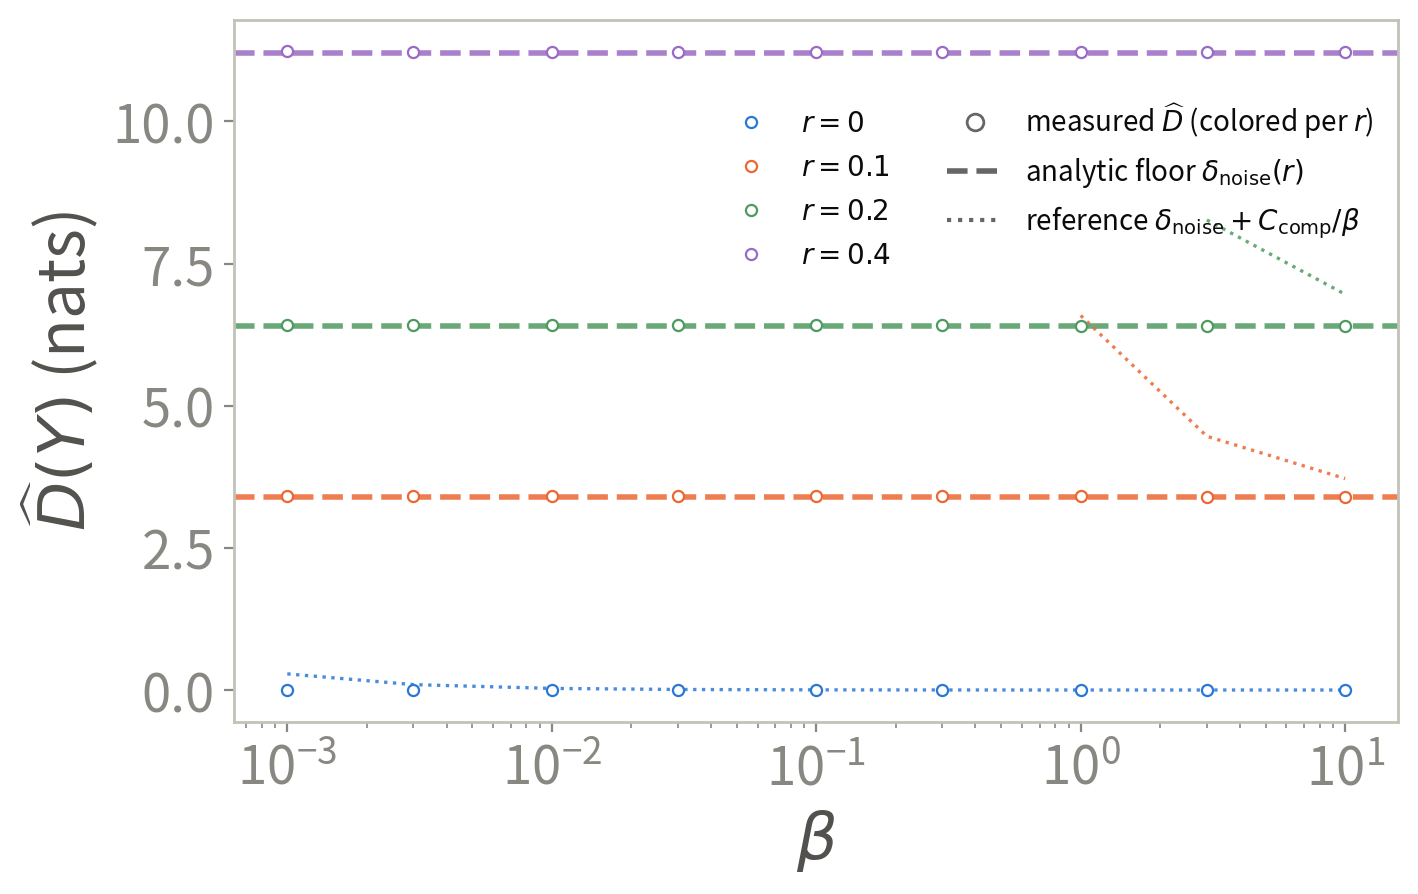
\includegraphics[width=0.32\linewidth]{figures/fig_noisy_appendix_i_varfixed.png}\hfill
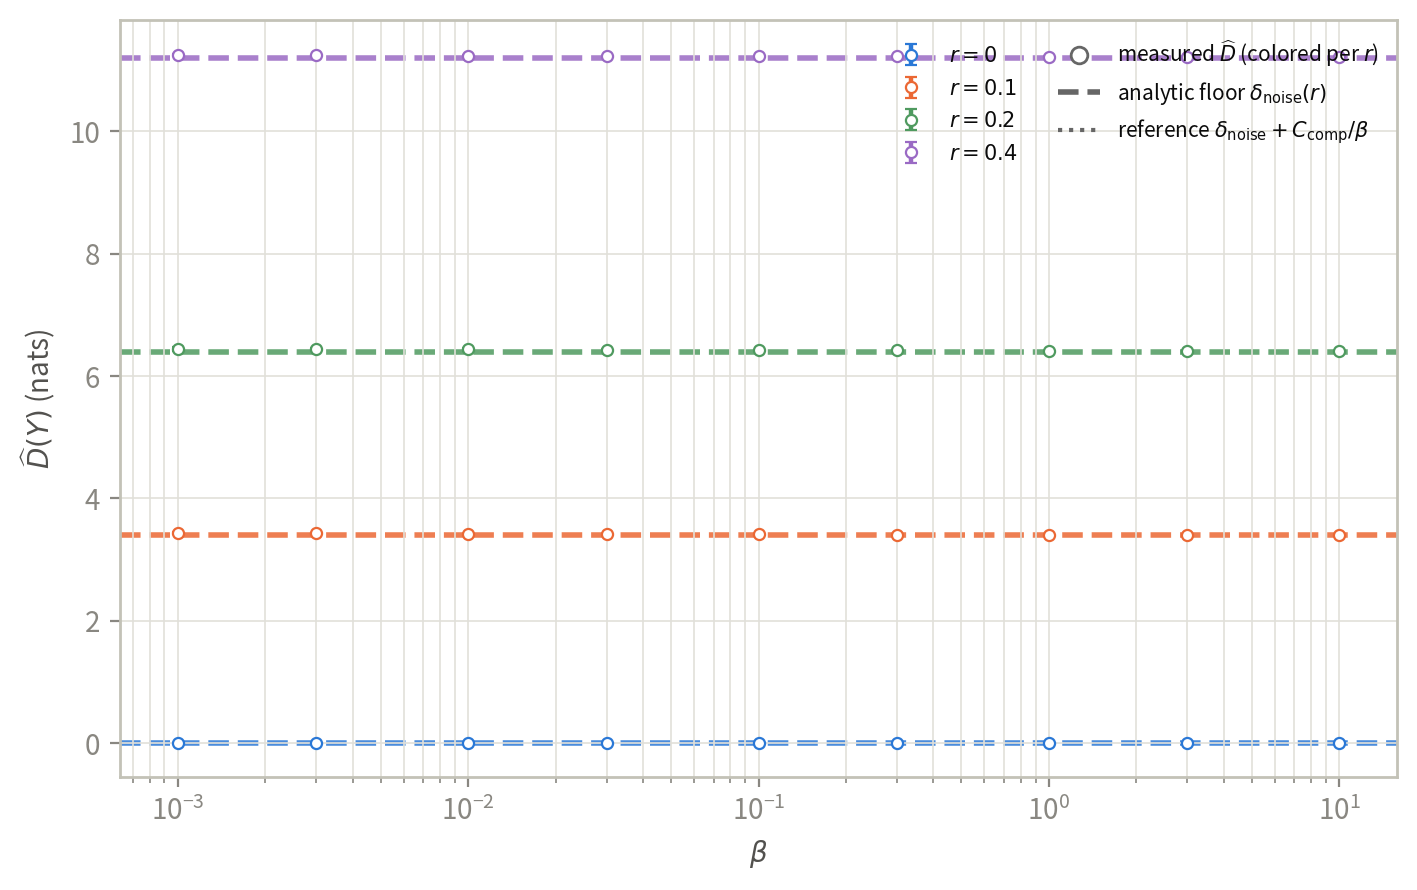
\includegraphics[width=0.32\linewidth]{figures/fig_noisy_appendix_ii_trainable.png}\hfill
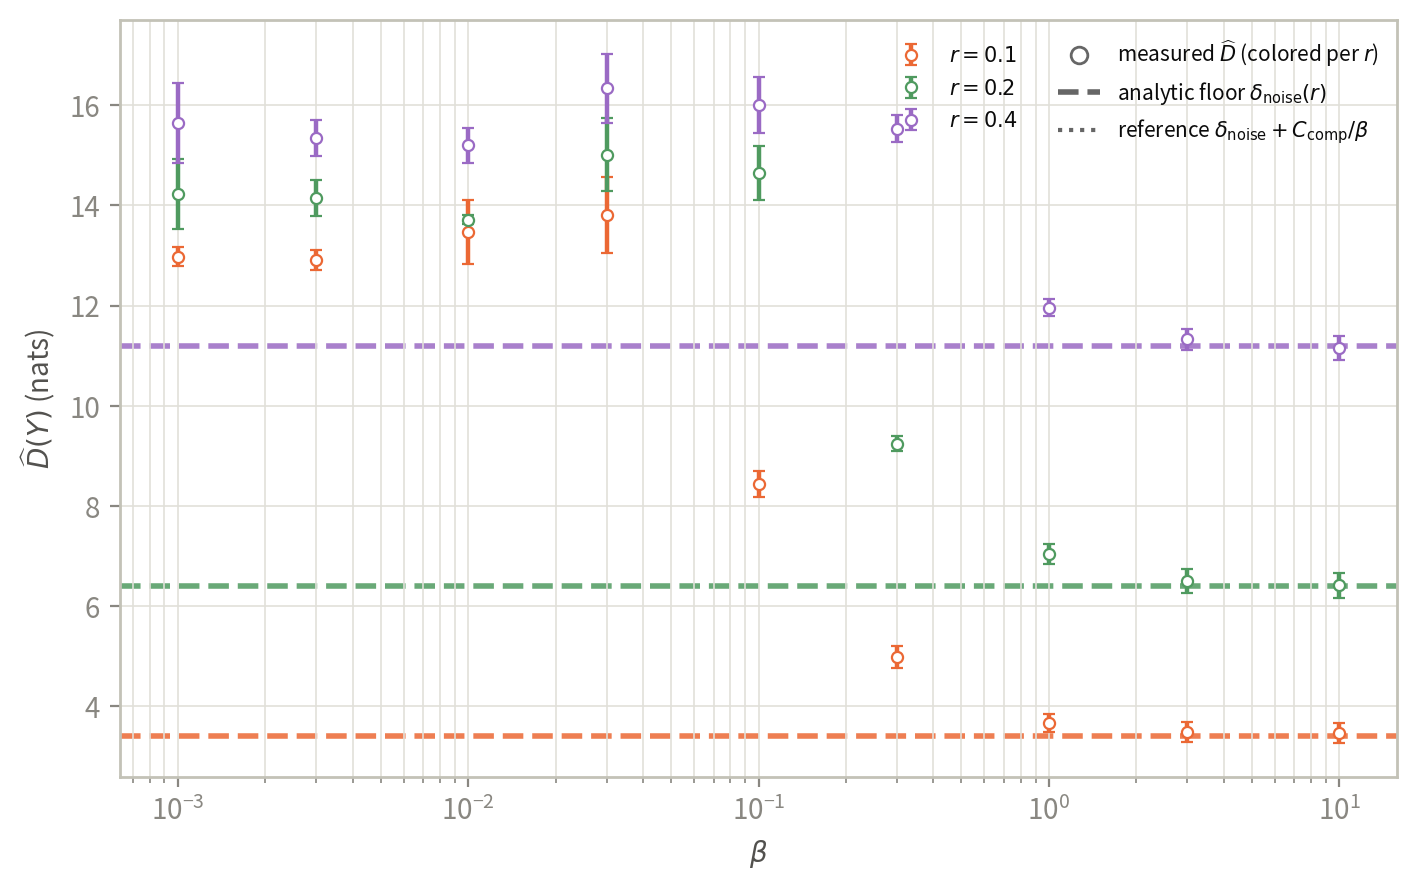
\includegraphics[width=0.32\linewidth]{figures/fig_noisy_appendix_iii_sampled.png}
\caption{Sensitivity analyses for the controlled label-ambiguity experiment.
(a) Posterior variance fixed to the prior variance. (b) Trainable polar
frame. (c) Labels sampled rather than integrated with their exact population weights;
failed comparator-gate configurations are marked. Dashed lines denote the analytic
population ambiguity floors. Points are means and error bars are standard deviations
over five seeds.}
\label{fig:noisy-alignment-sensitivity}
\end{figure*}

\subsection{Direct mismatch definitions and separation diagnostics}
\label{app:direct-mismatch}

This section collects the diagnostic panels deferred from
Section~\ref{sec:direct-mismatch}: the decoupling scatter, the separation-bound and
slack readings, and the regression diagnostics, together with the finite-bin
definitions. All statistics are first computed within each seed and then aggregated
across the five seeds; class or bin pairs are not treated as independent
replicates. The per-class Jensen check and the per-pair separation bound are
verified numerically on every scale, $\beta$, seed, and class (no violation exceeds
$10^{-6}$). Every checkpoint in both requested grids is present, and no collapse or
variance-explosion point is removed.

The deferred classification panels complete the picture
(Fig.~\ref{fig:direct-mismatch-deferred}). The decoupling scatter (a) shows MC-10
accuracy staying within $82$--$86\%$ while $\widehat D$ spans three orders of
magnitude: mechanism and task metric are decoupled. Panel (b) shows the raw bound
rising toward the declared $\sqrt2a$ exactly where the mismatch corrections shrink,
so the slack narrows where the bound is informative; CEB's mismatch is plotted
descriptively, without a bound or slack entries, since its reference has no declared
$\Delta$. The
slack percentiles (c) stay non-negative at every reported point: the bound is
consistent but conservative.

\begin{figure*}[t]
\centering
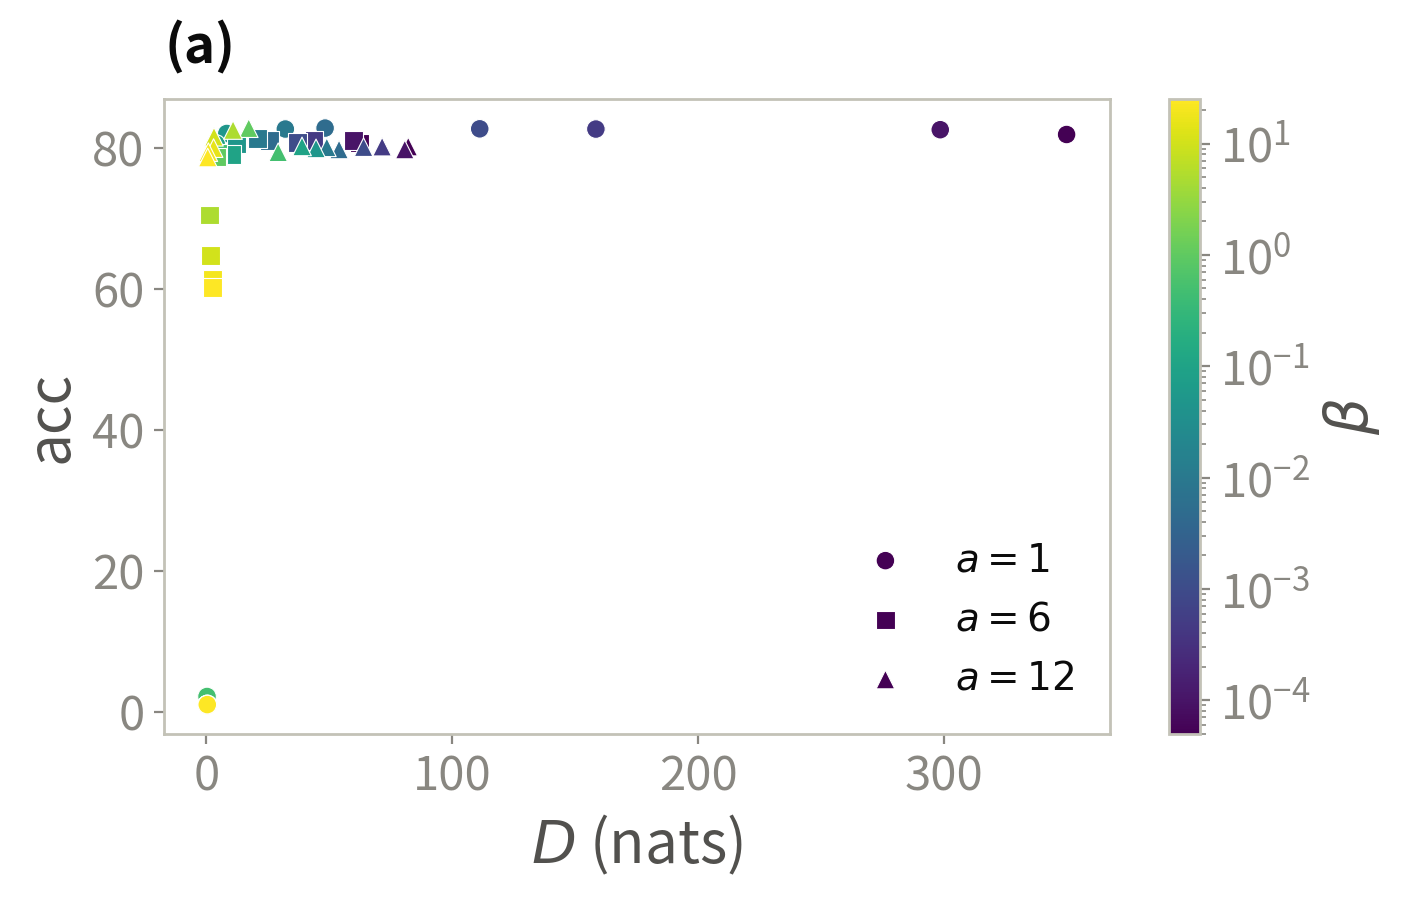
\includegraphics[width=0.24\linewidth]{figures/fig_mismatch_b_imagenet100_acc_vs_d.png}\hfill
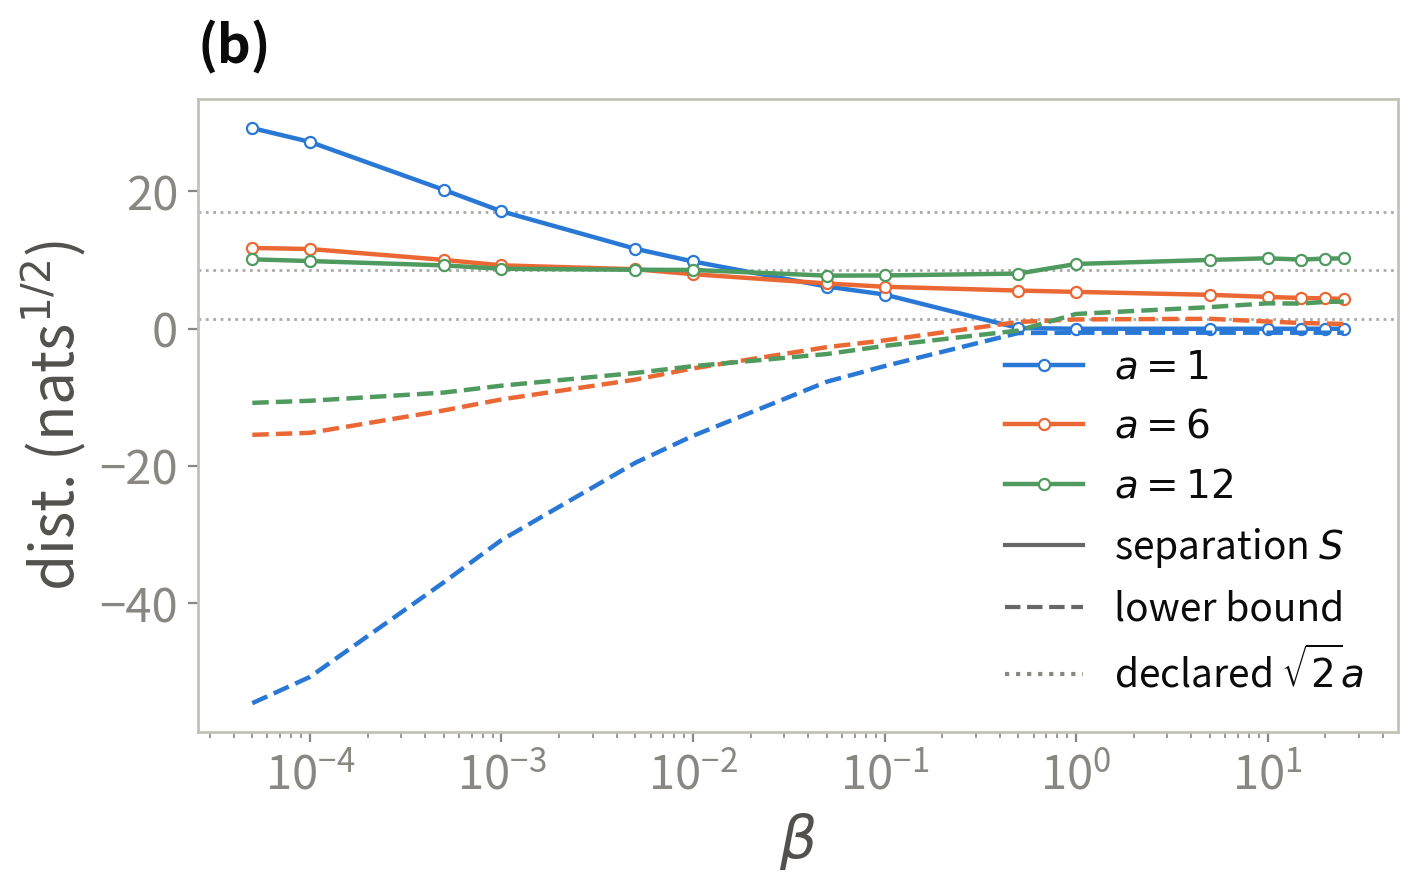
\includegraphics[width=0.24\linewidth]{figures/fig_mismatch_appendix_cls_i_separation_beta.png}\hfill
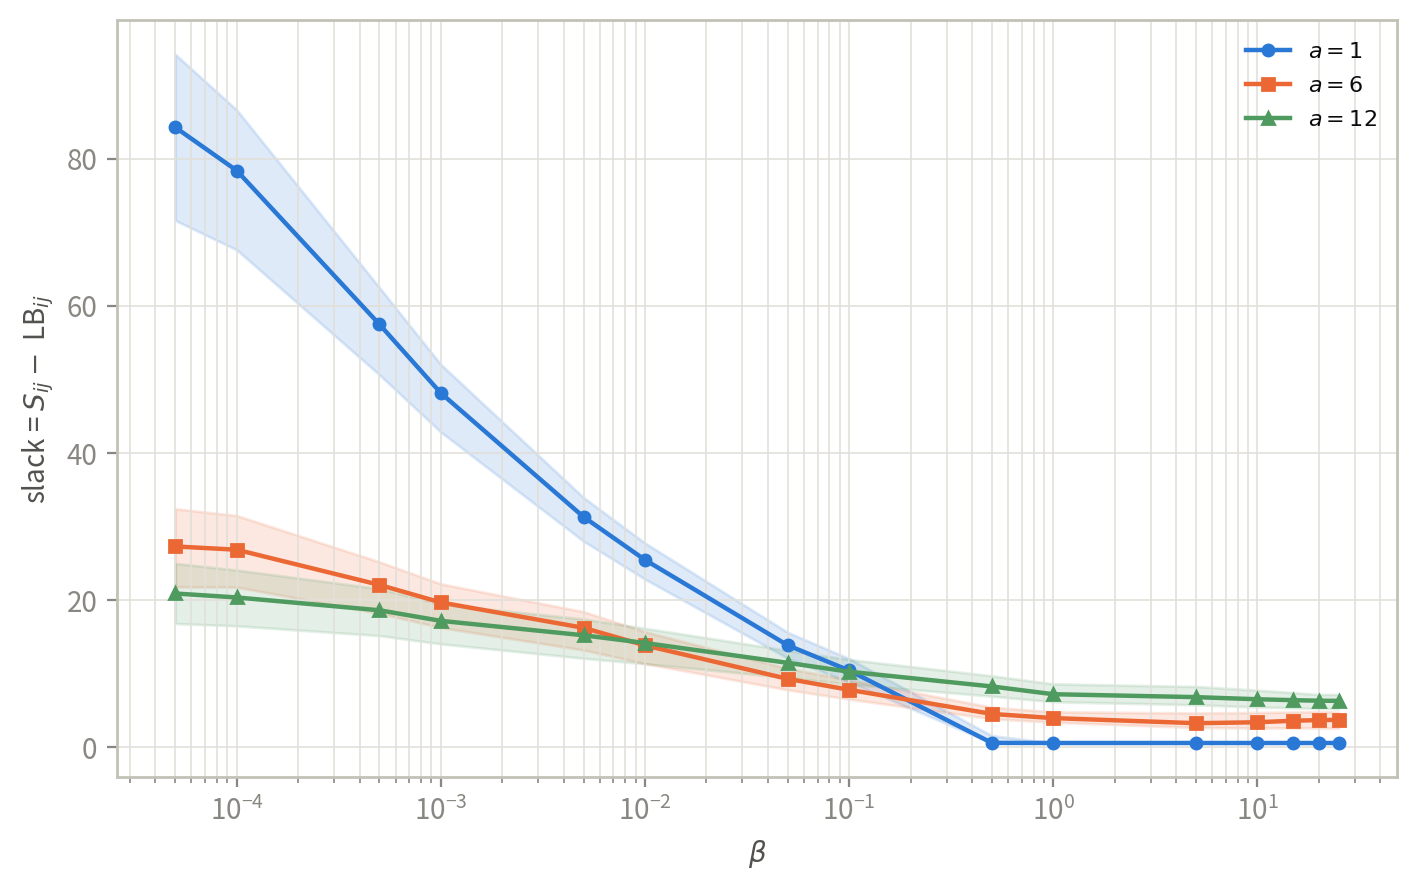
\includegraphics[width=0.24\linewidth]{figures/fig_mismatch_appendix_cls_iii_slack.png}\hfill
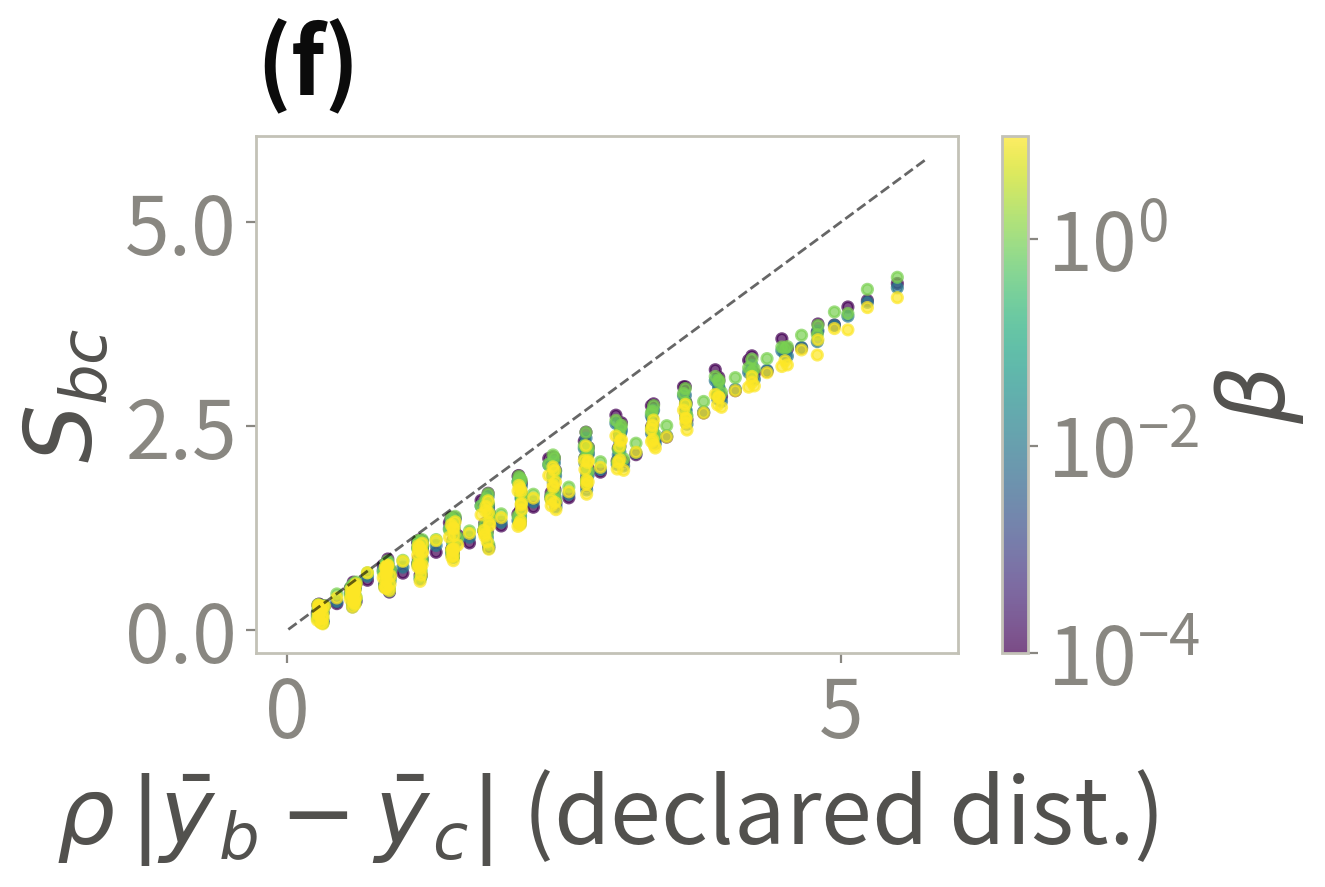
\includegraphics[width=0.24\linewidth]{figures/fig_mismatch_appendix_reg_binscatter.png}
\caption{Direct mismatch diagnostics deferred from the main text. (a) MC-10
accuracy against $\widehat D$ (color $=\beta$, marker $=a$). (b) Mean separation
(solid) and raw lower bound (dashed) against $\beta$; gray dotted: CEB,
descriptive. (c) Slack percentiles. (d) Cal.\ Housing bin-pair separation against
the declared prior distance at $\rho=6$ (color $=\beta$; identity line: exact
transfer). Means and standard deviations are over five seeds; no checkpoint is
omitted.}
\label{fig:direct-mismatch-deferred}
\end{figure*}

\paragraph{Regression.} We partition the standardized test labels into $20$
equal-width bins and merge any bin containing fewer than $30$ examples. Let
$\bar y_b$ be the mean label of bin $B_b$, $\widehat m_b$ its posterior center,
$\widehat D_b$ its average sample-to-own-anchor mismatch, and
$h_b:=\operatorname{diam}(B_b)$. The finite-bin lower bound is
\begin{equation}
\widehat{\mathrm{LB}}_{bc}
=\rho|\bar y_b-\bar y_c|
-\sqrt{2\tau^2\widehat D_b}
-\sqrt{2\tau^2\widehat D_c}
-\rho(h_b+h_c),
\label{eq:empirical-regression-separation-bound}
\end{equation}
where the last term is the quantization correction of
Remark~\ref{rem:pgib-binning}. On Housing with $\rho=6$, mismatch falls from
$0.264$ to $0.026$, the axial slope remains $0.73$--$0.77$, and the mismatch is
almost entirely axial (about $0.2$ against $0.004$ off-axis), while $R^2$ changes
only from $0.786$ to $0.767$ over the sweep: a tenfold mismatch reduction need not
imply a comparable task-metric gain. Figure~\ref{fig:direct-mismatch-deferred}d
plots the actual bin-center distances against the declared isometric distances at
$\rho=6$: the cloud hugs a line of slope $0.73$--$0.77$ below the identity line at
all four $\beta$ values, so the posterior follows the declared metric structure at
about three quarters of its scale, and the scale-transfer ratio is essentially
$\beta$-invariant. After the quantization correction, $43\%$ of bin pairs retain a
positive bound. Figure~\ref{fig:direct-mismatch-housing} shows the two regression
sweep panels: the mismatch--$\beta$ curves with their axial/off-axis decomposition
(the dotted off-axis contribution stays below $0.01$ nats, so the posterior lies
essentially on the declared axis), and the $R^2$-against-$\widehat D$ scatter whose
band stays within $0.75$--$0.79$ while $\widehat D$ spans orders of magnitude.

\begin{figure*}[t]
\centering
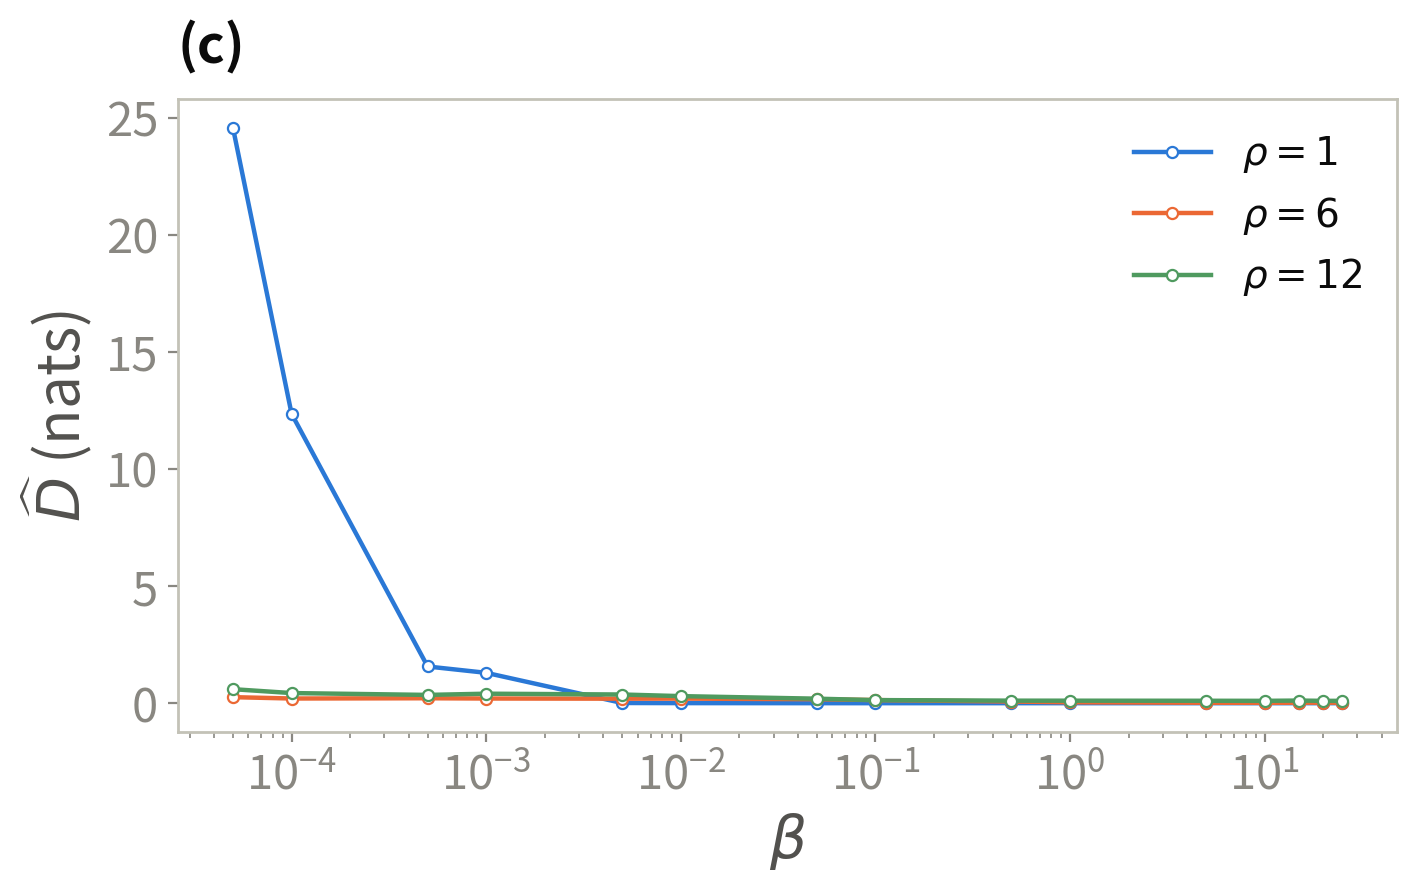
\includegraphics[width=0.48\linewidth]{figures/fig_mismatch_c_housing_d_beta.png}\hfill
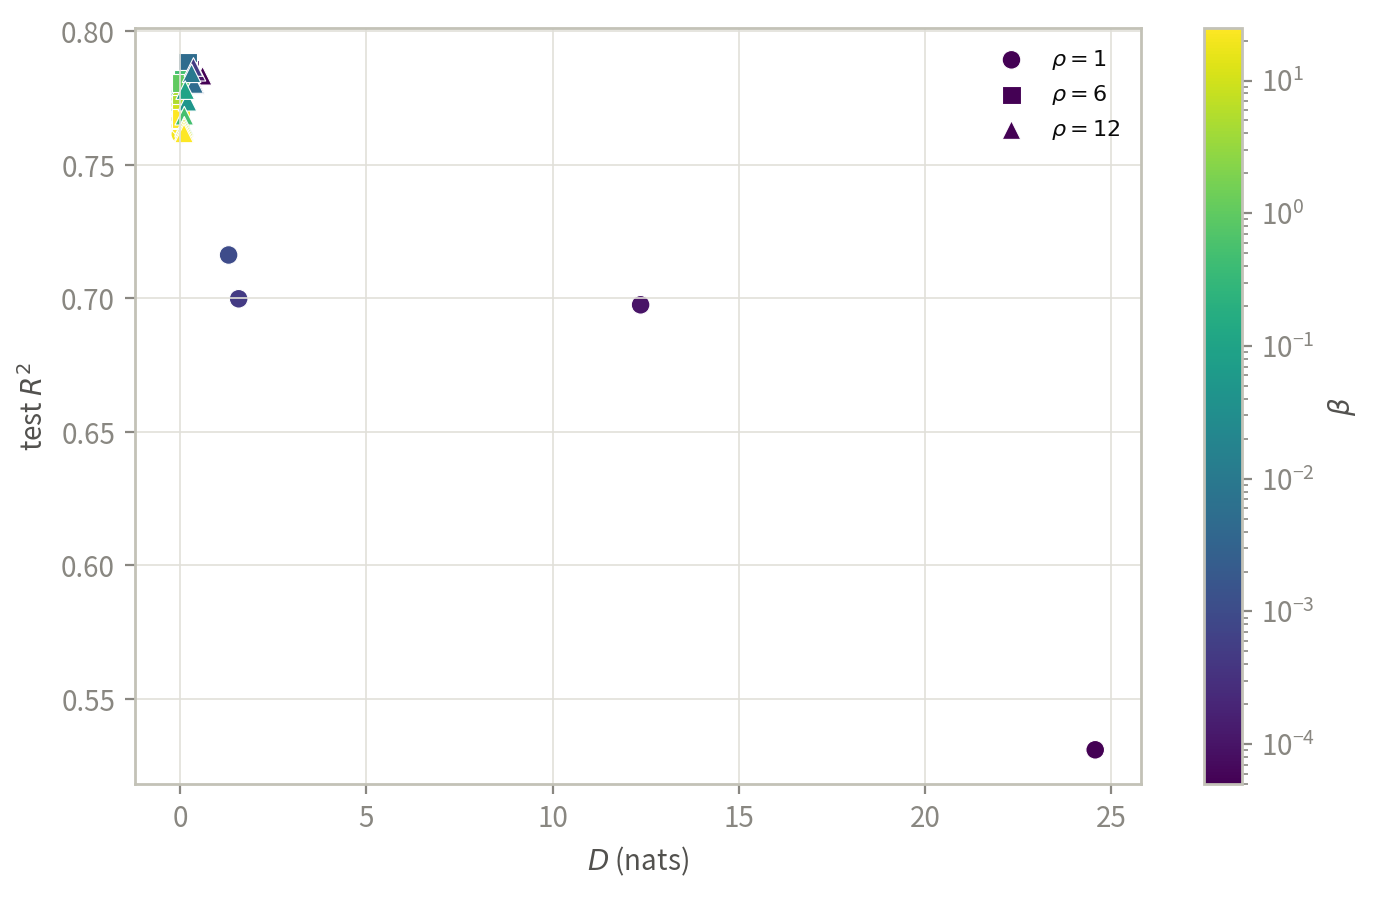
\includegraphics[width=0.48\linewidth]{figures/fig_mismatch_d_housing_r2_vs_d.png}
\caption{Cal.\ Housing mismatch sweep panels (deferred from the main text). (a)
Anchor mismatch $\widehat D$ against $\beta$, by isometric scale $\rho$, decomposed
into axial and off-axis contributions. (b) Test $R^2$ against $\widehat D$; color
denotes $\beta$ and marker shape $\rho$. Means and standard deviations are over five
seeds; no checkpoint is omitted.}
\label{fig:direct-mismatch-housing}
\end{figure*}

\paragraph{Normalization and variance extremes.} The empirical mismatch normalizes
by the declared prior variance $\tau^2=1$, whereas the
exact Gaussian KL uses every sample's and coordinate's own posterior variance
$\sigma^2_\phi(x)$. They therefore need not coincide: averaged over the ImageNet-100
grid, $\widehat D=41.2$, the KL mean term is $46.5$, and the KL variance term is
$51.4$. On Housing, a small number of weak-compression, large-$\rho$ posterior
variance explosions raise the across-grid mean KL variance term to $2.8\times10^6$;
these checkpoints remain in all plots. The unnormalized axial/off-axis components and
total KL are therefore reported alongside $\widehat D$.

\subsection{Main results with standard deviations}
\label{app:main-std}

Tables~\ref{tab:main_result_std_baselines} and~\ref{tab:main_result_std_variants}
report the same configurations as the main table with standard deviations over
runs, split by column groups for width (the baselines table includes NCBD and the
variants table includes AdaCap); bold and underline follow the same
mean-based rule as Table~\ref{tab:main_result}.

% 主结果表（带标准差）：由 paper/make_table.py 从 tune_results/*.html 自动生成，请勿手改。
% 因 8 方法列 × (均值±std) 超出页宽，按列拆为两张表：
% (a) baselines（Base/VIB/SVIB/NIB，tab:main_result_std_baselines）；
% (b) CEB/DVCCA 与 GPB/GPB-L（tab:main_result_std_variants，竖线分隔同主表）。
% 每表含全部 12 行；分类 Acc（%）、回归 R²，单元格为均值±std；
% 加粗/下划线按该行全部 8 列的均值判定（与 main_result.tex 一致）；
% 表尾排名行省略（与主表重复）。
\begin{table*}[t]
\centering
\caption{Test accuracy (\%) and test $R^2$ with standard deviations over runs: the plain backbone and the variational baselines; same configurations as Table~\ref{tab:main_result}.}
\label{tab:main_result_std_baselines}
\small
{
\setlength{\tabcolsep}{2pt}
\begin{tabular}{llcccc}
\hline
Dataset & Backbone & Base & VIB & SVIB & NIB \\
\hline
MNIST & MLP & 98.33$\pm$0.12 & 98.28$\pm$0.11 & 98.15$\pm$0.13 & 98.27$\pm$0.07 \\
MNIST & CNN & 99.13$\pm$0.05 & 99.28$\pm$0.09 & 99.23$\pm$0.03 & 99.22$\pm$0.06 \\
ImageNet-100 & MLP & 83.12$\pm$0.14 & 82.84$\pm$0.44 & 83.02$\pm$0.37 & 82.35$\pm$0.27 \\
ImageNet-100 & CNN & 83.40$\pm$0.13 & 82.94$\pm$0.37 & 83.11$\pm$0.86 & 82.91$\pm$0.35 \\
Cora & GCN & 87.68$\pm$0.46 & 86.83$\pm$0.28 & 86.46$\pm$1.87 & 86.35$\pm$0.68 \\
IMDb & RNN & 84.85$\pm$0.68 & 85.50$\pm$0.91 & 85.99$\pm$0.30 & 86.14$\pm$0.92 \\
AG News & RNN & \textbf{92.94$\pm$0.15} & 92.72$\pm$0.17 & 92.86$\pm$0.21 & 92.91$\pm$0.22 \\
\hline\hline
Cal. Housing & MLP & 0.7618$\pm$0.0238 & \underline{0.7901$\pm$0.0049} & 0.7897$\pm$0.0058 & 0.7862$\pm$0.0035 \\
STS-B & RNN & \textbf{0.2899$\pm$0.0113} & 0.2719$\pm$0.0164 & 0.2697$\pm$0.0202 & 0.2417$\pm$0.0221 \\
ZINC & GCN & \textbf{0.6348$\pm$0.0044} & 0.6339$\pm$0.0033 & 0.6325$\pm$0.0026 & 0.6178$\pm$0.0099 \\
AgeDB & MLP & 0.2180$\pm$0.0409 & 0.3173$\pm$0.0101 & \underline{0.3385$\pm$0.0286} & 0.2710$\pm$0.0235 \\
AgeDB & CNN & 0.3914$\pm$0.0194 & 0.3342$\pm$0.1894 & 0.3323$\pm$0.1870 & 0.3337$\pm$0.1889 \\
\hline
\end{tabular}
}
\end{table*}
\par\smallskip
\begin{table*}[t]
\centering
\caption{Test accuracy (\%) and test $R^2$ with standard deviations over runs: CEB, DVCCA, and our method; same configurations as Table~\ref{tab:main_result}. GPB and GPB-L are separated from the references by the vertical rule.}
\label{tab:main_result_std_variants}
\small
{
\setlength{\tabcolsep}{2pt}
\begin{tabular}{llcc|cc}
\hline
Dataset & Backbone & CEB & DVCCA & GPB & GPB-L \\
\hline
MNIST & MLP & \underline{98.43$\pm$0.08} & 98.24$\pm$0.17 & \textbf{98.54$\pm$0.09} & \underline{98.43$\pm$0.07} \\
MNIST & CNN & 99.30$\pm$0.05 & 99.29$\pm$0.10 & \textbf{99.32$\pm$0.05} & \underline{99.31$\pm$0.05} \\
ImageNet-100 & MLP & 82.77$\pm$0.22 & 82.99$\pm$0.43 & \textbf{84.40$\pm$0.21} & \underline{84.01$\pm$0.23} \\
ImageNet-100 & CNN & 82.97$\pm$0.67 & 83.21$\pm$0.70 & \textbf{86.08$\pm$0.21} & \underline{84.88$\pm$0.80} \\
Cora & GCN & 86.27$\pm$0.38 & 86.90$\pm$0.94 & \textbf{88.12$\pm$0.55} & \underline{87.86$\pm$0.87} \\
IMDb & RNN & 85.55$\pm$0.73 & 85.69$\pm$0.23 & \underline{86.84$\pm$0.57} & \textbf{86.99$\pm$0.35} \\
AG News & RNN & 92.83$\pm$0.11 & 92.78$\pm$0.15 & 92.87$\pm$0.12 & \underline{92.92$\pm$0.14} \\
\hline\hline
Cal. Housing & MLP & 0.7894$\pm$0.0018 & 0.7878$\pm$0.0048 & 0.7895$\pm$0.0051 & \textbf{0.7914$\pm$0.0034} \\
STS-B & RNN & 0.2668$\pm$0.0127 & 0.2713$\pm$0.0218 & \underline{0.2762$\pm$0.0152} & 0.2755$\pm$0.0134 \\
ZINC & GCN & 0.6257$\pm$0.0044 & 0.6294$\pm$0.0026 & \underline{0.6344$\pm$0.0031} & 0.6323$\pm$0.0016 \\
AgeDB & MLP & 0.3317$\pm$0.0251 & 0.3180$\pm$0.0228 & \textbf{0.3536$\pm$0.0076} & 0.3320$\pm$0.0080 \\
AgeDB & CNN & 0.3882$\pm$0.0275 & 0.3205$\pm$0.1811 & \textbf{0.4700$\pm$0.0072} & \underline{0.4388$\pm$0.0220} \\
\hline
\end{tabular}
}
\end{table*}
\par\smallskip


\subsection{Paired-difference confidence intervals}
\label{app:main-ci}

Tables~\ref{tab:main_result_ci_baselines}--\ref{tab:main_result_ci_external}
report, for each setting, the paired difference of GPB over every baseline
(GPB minus baseline) with a bootstrap $95\%$ confidence interval: the differences
are paired across the shared seeds, the interval is the percentile interval of
$B = 10{,}000$ resamples of the per-run differences (fixed seed, reproducible), and
the non-inferiority margin is $\delta = 0.2$ percentage points of accuracy or
$\delta = 0.005$ in $R^2$. Bold marks a lower bound above zero (significant
advantage) and $^{\dagger}$ a lower bound within the margin (tied); the best
configuration per method is the same as in the main table. The last table covers
the external non-IB baselines, NCBD on the classification settings and AdaCap on
the regression settings; the only interval lying entirely below zero is AdaCap on
ZINC ($-0.043$ $R^2$).

% 主结果差值 CI 表：由 paper/make_table.py 从 tune_results 自动生成，请勿手改。
% 行 = 12 个 setting；单元格 = GPB − baseline 的配对差值 [bootstrap 95% CI]
%（分类百分点、回归 R²）；加粗 = CI 下限 > 0（显著更优）、† = CI 下限 > −δ
%（非劣界 δ=0.2 百分点 / 0.005）记 tied；
% 同 seed 配对（run 顺序即 seed 0..N−1），bootstrap B=10000（固定 seed 0，百分位法）。
% 因 7 个差值列超页宽，按列拆两张表（baselines / ceb+dvcca+OPB-L）；表尾一行统计各列 */† 次数。
\begin{table*}[t]
\centering
\caption{Paired-difference 95\% confidence intervals of GPB over the plain backbone and VIB (GPB minus baseline, per setting; classification in percentage points, regression in $R^2$). Bold: lower CI bound above zero; $^{\dagger}$: lower bound within the non-inferiority margin $\delta$ (tied).}
\label{tab:main_result_ci_baselines}
\small
{
\setlength{\tabcolsep}{1pt}
\begin{tabular}{llcc}
\hline
Dataset & Backbone & Base & VIB \\
\hline
MNIST & MLP & \textbf{+0.2 [+0.2, +0.3]} & \textbf{+0.3 [+0.2, +0.3]} \\
MNIST & CNN & \textbf{+0.2 [+0.2, +0.2]} & +0.0 [-0.0, +0.1]$^{\dagger}$ \\
ImageNet-100 & MLP & \textbf{+1.3 [+1.2, +1.4]} & \textbf{+1.6 [+1.4, +1.9]} \\
ImageNet-100 & CNN & \textbf{+2.7 [+2.5, +2.9]} & \textbf{+3.1 [+3.0, +3.4]} \\
Cora & GCN & +0.4 [-0.1, +1.1]$^{\dagger}$ & \textbf{+1.3 [+0.7, +1.7]} \\
IMDb & RNN & \textbf{+2.0 [+1.2, +2.7]} & \textbf{+1.3 [+0.6, +2.3]} \\
AG News & RNN & -0.1 [-0.2, +0.0]$^{\dagger}$ & \textbf{+0.2 [+0.1, +0.2]} \\
\hline\hline
Cal. Housing & MLP & \textbf{+0.028 [+0.008, +0.048]} & -0.001 [-0.005, +0.003]$^{\dagger}$ \\
STS-B & RNN & -0.014 [-0.022, -0.006] & +0.004 [-0.017, +0.022] \\
ZINC & GCN & -0.000 [-0.003, +0.002]$^{\dagger}$ & +0.001 [-0.004, +0.004]$^{\dagger}$ \\
AgeDB & MLP & \textbf{+0.136 [+0.104, +0.167]} & \textbf{+0.036 [+0.026, +0.046]} \\
AgeDB & CNN & \textbf{+0.079 [+0.066, +0.091]} & \textbf{+0.136 [+0.043, +0.302]} \\
\hline
 &  & 8*/3† & 8*/3† \\
\hline
\end{tabular}
}
\end{table*}
\par\smallskip
\begin{table*}[t]
\centering
\caption{Paired-difference 95\% confidence intervals of GPB over SVIB and NIB (GPB minus baseline, per setting; classification in percentage points, regression in $R^2$). Bold/† as in the baselines table.}
\label{tab:main_result_ci_svib_nib}
\small
{
\setlength{\tabcolsep}{1pt}
\begin{tabular}{llcc}
\hline
Dataset & Backbone & SVIB & NIB \\
\hline
MNIST & MLP & \textbf{+0.4 [+0.3, +0.5]} & \textbf{+0.3 [+0.2, +0.3]} \\
MNIST & CNN & \textbf{+0.1 [+0.1, +0.1]} & \textbf{+0.1 [+0.1, +0.2]} \\
ImageNet-100 & MLP & \textbf{+1.4 [+1.1, +1.7]} & \textbf{+2.1 [+1.8, +2.2]} \\
ImageNet-100 & CNN & \textbf{+3.0 [+2.4, +3.9]} & \textbf{+3.2 [+2.9, +3.5]} \\
Cora & GCN & \textbf{+1.7 [+0.2, +3.4]} & \textbf{+1.8 [+1.1, +2.4]} \\
IMDb & RNN & \textbf{+0.8 [+0.2, +1.4]} & \textbf{+0.7 [+0.2, +1.2]} \\
AG News & RNN & +0.0 [-0.1, +0.1]$^{\dagger}$ & -0.0 [-0.2, +0.1]$^{\dagger}$ \\
\hline\hline
Cal. Housing & MLP & -0.000 [-0.006, +0.004] & +0.003 [-0.001, +0.009]$^{\dagger}$ \\
STS-B & RNN & +0.006 [-0.021, +0.028] & \textbf{+0.035 [+0.011, +0.058]} \\
ZINC & GCN & +0.002 [-0.001, +0.004]$^{\dagger}$ & \textbf{+0.017 [+0.010, +0.026]} \\
AgeDB & MLP & +0.015 [-0.010, +0.041] & \textbf{+0.083 [+0.062, +0.100]} \\
AgeDB & CNN & \textbf{+0.138 [+0.045, +0.303]} & \textbf{+0.136 [+0.040, +0.302]} \\
\hline
 &  & 7*/2† & 10*/2† \\
\hline
\end{tabular}
}
\end{table*}
\par\smallskip
\begin{table*}[t]
\centering
\caption{Paired-difference 95\% confidence intervals of GPB over CEB, DVCCA, and the free-head ablation OPB-L (GPB minus baseline, per setting; classification in percentage points, regression in $R^2$). Bold/† as in the baselines table.}
\label{tab:main_result_ci_variants}
\small
{
\setlength{\tabcolsep}{1pt}
\begin{tabular}{llccc}
\hline
Dataset & Backbone & CEB & DVCCA & OPB-L \\
\hline
MNIST & MLP & \textbf{+0.1 [+0.0, +0.2]} & \textbf{+0.3 [+0.2, +0.4]} & \textbf{+0.1 [+0.0, +0.2]} \\
MNIST & CNN & +0.0 [-0.0, +0.1]$^{\dagger}$ & +0.0 [-0.1, +0.1]$^{\dagger}$ & +0.0 [-0.0, +0.1]$^{\dagger}$ \\
ImageNet-100 & MLP & \textbf{+1.6 [+1.5, +1.7]} & \textbf{+1.4 [+1.1, +1.7]} & \textbf{+0.4 [+0.2, +0.5]} \\
ImageNet-100 & CNN & \textbf{+3.1 [+2.4, +3.7]} & \textbf{+2.9 [+2.4, +3.5]} & \textbf{+1.2 [+0.5, +1.9]} \\
Cora & GCN & \textbf{+1.8 [+1.5, +2.3]} & \textbf{+1.2 [+0.4, +1.9]} & +0.3 [-0.5, +1.3] \\
IMDb & RNN & \textbf{+1.3 [+0.3, +2.1]} & \textbf{+1.1 [+0.8, +1.5]} & -0.2 [-0.6, +0.5] \\
AG News & RNN & +0.0 [-0.1, +0.2]$^{\dagger}$ & +0.1 [-0.0, +0.2]$^{\dagger}$ & -0.0 [-0.2, +0.1]$^{\dagger}$ \\
\hline\hline
Cal. Housing & MLP & +0.000 [-0.003, +0.004]$^{\dagger}$ & +0.002 [-0.005, +0.009] & -0.002 [-0.005, +0.002] \\
STS-B & RNN & +0.009 [-0.009, +0.025] & +0.005 [-0.020, +0.026] & +0.001 [-0.019, +0.017] \\
ZINC & GCN & \textbf{+0.009 [+0.005, +0.011]} & \textbf{+0.005 [+0.002, +0.007]} & +0.002 [-0.001, +0.005]$^{\dagger}$ \\
AgeDB & MLP & \textbf{+0.022 [+0.006, +0.038]} & \textbf{+0.036 [+0.012, +0.057]} & \textbf{+0.022 [+0.019, +0.025]} \\
AgeDB & CNN & \textbf{+0.082 [+0.064, +0.099]} & \textbf{+0.149 [+0.065, +0.310]} & \textbf{+0.031 [+0.018, +0.046]} \\
\hline
 &  & 8*/3† & 8*/2† & 5*/3† \\
\hline
\end{tabular}
}
\end{table*}
\par\smallskip


\subsection{Information-plane panels for Cal.~Housing}
\label{app:info-plane-extra}

Figure~\ref{fig:info-plane-extra} completes panels (c)--(d) of
Fig.~\ref{fig:compression-main} in the main text with the regression setting, under
the same $\beta$ grid, axis
conventions, and five runs per point; here
$I(Y;Z)$ is the Gaussian approximation
$\tfrac12 \ln\bigl(\mathrm{Var}(y)/\mathrm{Var}(y-\hat y)\bigr)$, a heuristic
rather than a bound. On Cal.~Housing this approximation consistently reads
above the InfoNCE bound, so the certificate panel reflects the estimator gap
rather than the geometry; the information plane remains informative: CEB
compresses itself off the task ($R^2 = 0.49$ at $\beta = 0.1$, $0.18$ at
$\beta = 0.5$) while every EPB curve keeps $R^2 \ge 0.76$ flat out to
$\beta = 25$.

\begin{figure*}[t]
\centering
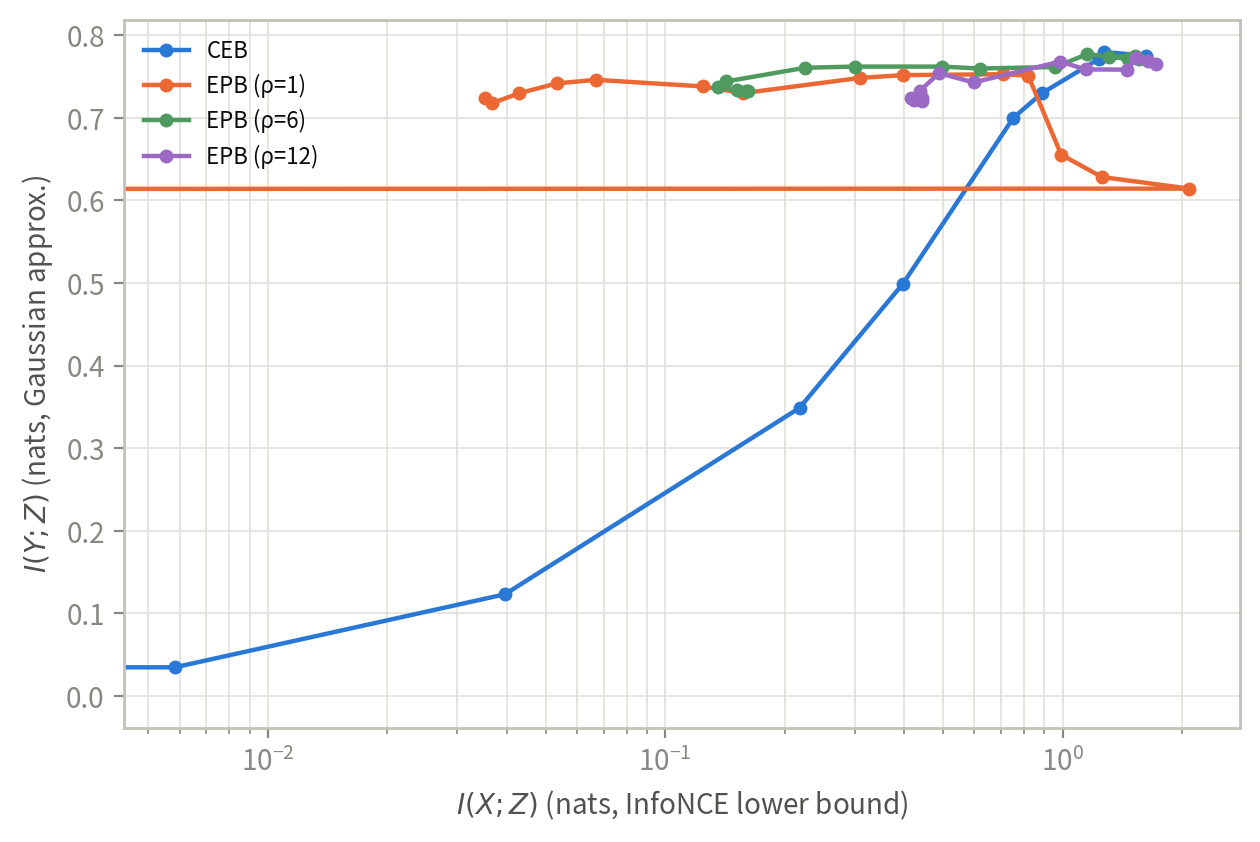
\includegraphics[width=0.48\linewidth]{figures/fig_info_plane_housing.png}\hfill
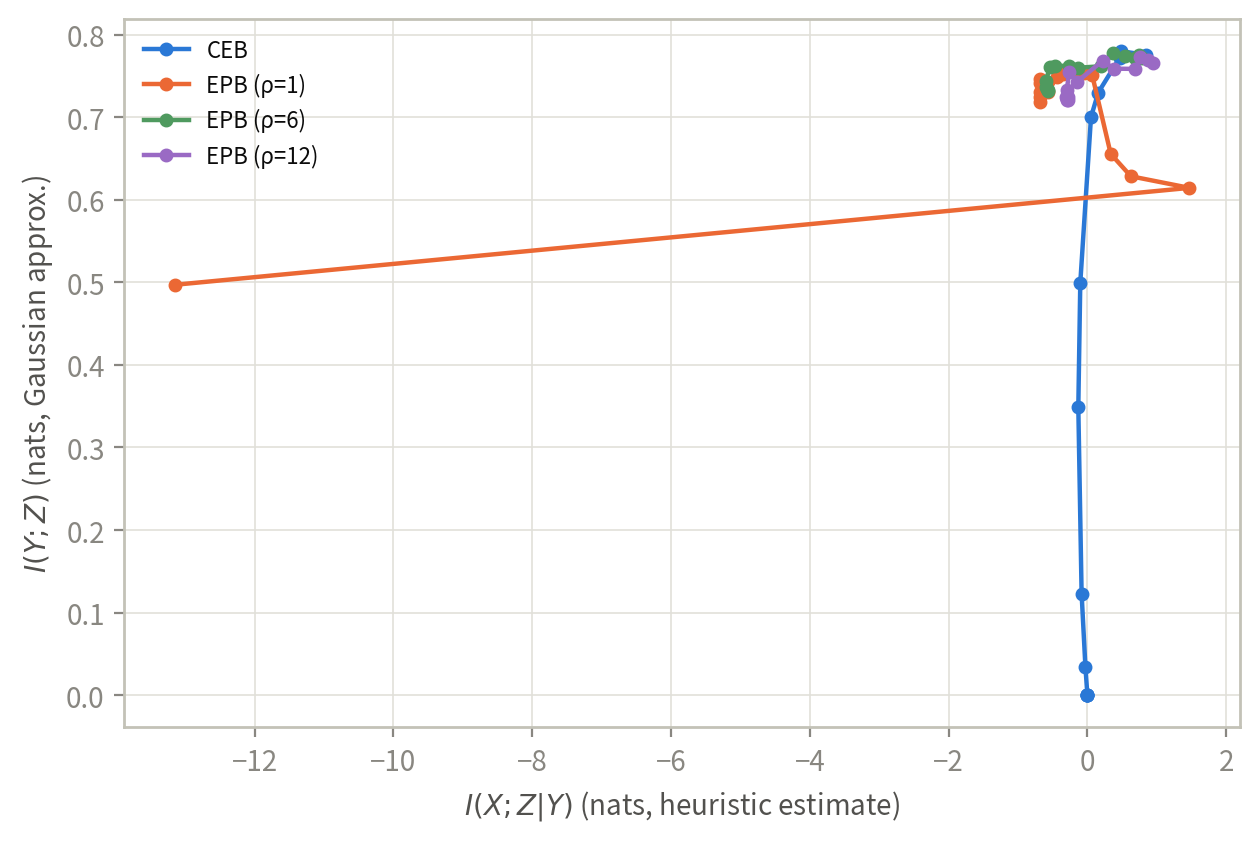
\includegraphics[width=0.48\linewidth]{figures/fig_certificate_plane_housing.png}
\caption{Information plane (a) and certificate plane (b) for Cal.~Housing,
companion panels to Fig.~\ref{fig:compression-main}(c,d): identical estimators,
$\beta$ grid (log $x$-scale in (a); linear where the estimated residual turns negative
in (b)), five runs per point, lines connect $\beta$ in ascending order. CEB
one curve per panel; EPB three ($\rho \in \{1, 6, 12\}$).}
\label{fig:info-plane-extra}
\end{figure*}

% =====================================================================




\end{document}
